\documentclass{tex/kdp} % utf8,utf8x
%\usepackage[utf8]{inputenc}

\usepackage{tex/mplstyle} 
\usepackage{tex/customcolors}
\usepackage{tex/mycommands}

% Title
\title{Matplotlib for Storytellers}
\author{\scalebox{0.91}{By: \link{https://github.com/alexanderthclark}{Alexander Clark}}}
\vspace{4cm}
\date{\scalebox{.8}{This version: \today}}

% leanpub cover image
% https://commons.wikimedia.org/wiki/File:William_Blake_-_The_First_Book_of_Urizen,_Plate_8,_%22In_Living_Creations_Appear%27d....%22_(Bentley_5)_-_Google_Art_Project.jpg
% Public Domain

% name the list of listings 
\renewcommand\lstlistlistingname{Code} 
%\setcounter{tocdepth}{1}


\begin{document}

\frontmatter
\maketitle

% Copyright stuff %\doclicenseThis
\vfill 
\begin{figure}
    \centering
    
\includegraphics[width = .3\textwidth]{Images/by-nc-sa.png}
    %\caption{Caption}
    %\label{fig:my_label}
\end{figure}

\noindent This text is released under the \link{https://creativecommons.org/licenses/by-nc-sa/4.0/deed.en}{Creative Commons Attribute-NonCommercial-ShareAlike 4.0 International} License.

\smallskip
\noindent The code is released under the MIT license. 

\smallskip
\noindent The front cover image (on \link{https://leanpub.com/mplforstorytellers}{Leanpub}) is from The First Book of Urizen, Plate 8, ``In Living Creations Appear'd....'' by William Blake (public domain). 

\bigskip 
\noindent Find more material on this book's GitHub page and on YouTube.

\noindent \link{https://github.com/alexanderthclark/Matplotlib-for-Storytellers}{github.com/alexanderthclark/Matplotlib-for-Storytellers}\\
\link{https://www.youtube.com/channel/UC7zSpQsXo4ezksvHaGYTvzg}{youtube.com/@alexanderthclark}

\tableofcontents
\vfill
%% Add list of listings for code
%\pagebreak

\lstlistoflistings
\bigskip

\noindent All code and data files are (\textcolor{red}{not yet}) available on the book's \link{https://github.com/alexanderthclark/Matplotlib-for-Storytellers}{GitHub repository}. Note I exclude imports from the Python files in the main text. The imports below should cover the entire text. All of these should be included if you installed Anaconda, except for the ternary library, which I comment out below. When saving figures, I also sometimes run \code{fig.tight_layout()}, which is not always included in the Python files. See \texttt{Figure-Dev.ipynb} which contains the complete code for every figure.


\pyfiletoc{imports.py}


\newpage

\chapter*{Preface}
\addcontentsline{toc}{chapter}{Preface}
\markboth{}{Preface}


\section*{Technical Notes and Prerequisites}
\addcontentsline{toc}{section}{Technical Notes and Prerequisites}
I use Python 3.9 and matplotlib 3.7.1. I also make use of Jupyter notebook cell magics. I assume familiarity with basic Python programming, NumPy, pandas, and even matplotlib. In Part \ref{part:prose}, the premise is that you can make a plot, but now you want to polish it. Other parts assume less background knowledge. For those needing to review some Python before approaching this text, I recommend \link{https://jakevdp.github.io/WhirlwindTourOfPython/}{\emph{A Whirlwind Tour of Python}} and \link{https://jakevdp.github.io/PythonDataScienceHandbook/}{\emph{Python Data Science Handbook}}, both by Jake VanderPlas.

%Because this is \emph{Matplotlib for Haters}, I assume some exposure to matplotlib so that I won't explain the most basic constructions. 
%upgraded to 3.71 from 3.5.1 on July 7 2023

\section*{Why Matplotlib?}
\addcontentsline{toc}{section}{Why Matplotlib?}
%These notes are an outgrowth of my general Python for Data Analysis lecture notes, expanding what was covered in under two two-hour lectures to what will take more. 
Though a bit aged, matplotlib is the standard in Python. matplotlib is integrated with pandas and Seaborn is based off matplotlib. You might prefer Plotnine if you already know R's ggplot2. You might prefer to leave Python and use D3 if you know javascript. You might prefer Microsoft Excel if you want consultants in your audience to feel at home.

I recommend matplotlib to anyone who is already committed to working in Python (and with the Python community) and values reproducibility and customizability. By the time we get to Part \ref{part:poetry}, we'll be drawing more than plotting. This allows for more creativity than Excel allows and we'll maintain a reproducible Python-only workflow. 

\section*{Good Visualization is Like Good Writing}\label{sec:writing}
\addcontentsline{toc}{section}{Good Visualization is like Good Writing}
% Visualization 
% Prose, Poetry, and the Invasion of Your Mind by Ready-made Phrases
% Good Visualization is like Good Writing

This book isn't a guide to visualization design, but we must consider, at least briefly, what makes for good visualization and then why you might find matplotlib useful in that pursuit. 

Data visualization is a form of communication not much different than writing. Cole Nussbaumer Knaflic's \emph{Storytelling with Data} parallels writing style guides like Sir Ernest Gowers' \emph{The Complete Plain Words}. They both emphasize clarity and stripping out what is not essential. Matplotlib doesn't offer any unique advantage in pursuing clarity. Instead, the advantage is a tactical one. Matplotlib will expand your options. Sometimes straightforward prose is appropriate and sometimes only poetry will be stirring enough to capture your audience's attention. There exist prosaic visualizations and poetic visualizations with all the same tradeoffs. 

Prose is precise and direct. Poetry has a certain beauty that invites interest and mediates higher truths. The familiar bar chart is prose, plainly reporting the numbers that need to be reported. Your boss will appreciate prose in a routine meeting. But imagine the king must wrestle with a difficult truth. Prose won't do. Only a jester or a Shakespearean fool can deliver the message and only by rhyme and riddle. So it may be with your C-level audience. The small truths of your bar charts don't matter to a busy CEO. Easier said than done, but capture your CEO's attention with a poetic visualization that might sacrifice some precision for its larger message. 

%In writing, we develop our capacity for good prose and good poetry by learning the fundamentals and then by practice and reading. It's a larger task than this book tackles, but this book aims to better your matplotlib fundamentals.

A hurdle to crafting good visualizations is being limited to a short menu of cookie cutter graphics, whatever is available in Excel, a dashboard tool, or from a limited knowledge of matplotlib. Ahead of us is the chance to break free from those cookie cutter, ready-made visuals. In writing, George Orwell made good note of the ``invasion of one's mind by ready-made phrases,'' in his worthwhile essay \textit{Politics and the English Language}: 

\begin{displayquote}
\textins{Ready-made phrases} will construct your sentences for you---even think your thoughts for you, to a certain extent---and at need they will perform the important service of partially concealing your meaning even from yourself.
%\hspace{10pt} From \textit{Politics and the English Language} by George Orwell
\end{displayquote}

\noindent The important point here is that the unimaginative application of ready-made visualizations, just like phrases, can conceal your meaning from yourself, not to mention your audience, and create a monotonous presentation of bar chart after bar chart. 

The parallels between writing and making visuals go one level further. If you want to \emph{become} a good writer, you will learn grammar, read good writers who came before you, write a lot, and skirt the rules a bit as you find your voice. In other words, you will do many things. Data visualization is no different. In what follows, you will begin to master just one thing, the technical grammar of matplotlib. %Go forth, and imagine Orwell has taken up data science in the afterlife and his ghost is watching you prepare your visualizations.

%I have no idea what this graph from @F1 (Formula 1) on Twitter is supposed to convey. 
%\begin{center}
%    \includegraphics[width = .55\textwidth]{F1}
%\end{center}
%from philosopher Roger Scruton in mind, ``Art moves us because it is beautiful, and it is beautiful because it means something. It can be meaningful without being beautiful; but to be beautiful it must be meaningful.''

%\noindent \textbf{\emph{Resources and Inspiration}}:
\section*{Resources and Inspiration}
\addcontentsline{toc}{section}{Resources and Inspiration}
Before you dive in, you ought to get excited about data visualization. While there is a glaring lack of major museum space devoted to data visualization (I just recall a disappointing exhibit at the Cooper Hewitt), you will find many wonderful displays if you only keep your eyes peeled. 
 
If you like to listen to people talk about data visualization, I recommend the \link{https://datastori.es}{Data Stories podcast}. 

If you'd like to start by reading one of the pioneers, check out \link{https://www.edwardtufte.com/tufte/}{Edward Tufte}, who continues to write new material. For more explicit or domain-specific guidance than Tufte might provide, see \link{https://www.storytellingwithdata.com/book/downloads}{Storytelling with Data} by Cole Nussbaumer Knaflic or \link{http://cup.columbia.edu/book/better-data-visualizations/9780231193115}{Better Data Visualization} by Jonathan Schwabish. Many of Schwabish's main themes are also communicated more briefly in \cite{schwabish2014economist}. I have limited patience for how-to guides when they edge toward being overly prescriptive (I've never read any books on how to write well either), but I've profited from these titles. They are useful for their treatment of fundamentals like preattentive processing and surfacing more variety in visualizations, helping to inspire a richer repertoire. Knaflic's book is oriented toward business professionals and Schwabish adds his own public policy background. As a result, Knaflic concentrates on what I call prosaic visuals  and Schwabish pushes further into the realm of poetry. Schwabish discusses the tradeoffs between standard and nonstandard graphs, noting that novelty can encourage more active processing, providing further justification for using a less accurate graph in select, exploratory cases.
%Media outlets 

Media outlets like the New York Times and Wall Street Journal make usually good use of data visualization. Take appropriate inspiration these sources and from the  \link{https://www.reddit.com/r/dataisbeautiful}{r/DataIsBeautiful} and \link{https://www.reddit.com/r/dataisugly/}{r/DataIsUgly} subreddits.

There is also a good Data Visualization section in \link{https://aeturrell.github.io/coding-for-economists/intro.html}{\emph{Coding for Economists}} by Arthur Turrell. For a more advanced treatment of matplotlib, check out \link{https://github.com/rougier/scientific-visualization-book}{Scientific Visualization: Python + Matplotlib}.


\section*{Text Organization}
\addcontentsline{toc}{section}{Text Organization}
Continuing the \hyperref[sec:writing]{parallel to writing}, I have built this text around two main parts: \hyperref[part:prose]{Prose} and \hyperref[part:poetry]{Poetry}, though the distinction between prose and poetry is surely less exact than the division I've created. Prose, or Part \ref{part:prose}, focuses on the fundamentals of customizing plots through the object-oriented interface. This section attempts to be reasonably thorough in breadth while providing only a minimal effective dose in depth. Then, after a mathematical interlude in Part \ref{part:math}, we reach poetry in Part \ref{part:poetry}. There can be no comprehensiveness to this section. I provide a guide to drawing in matplotlib, mostly with various \link{https://matplotlib.org/stable/api/artist_api.html\#artist-class}{artist} objects. The mathematical interlude is there for those who would like to review some trigonometry I use. Then, I introduce two special (for fun) topics in Part \ref{part:topics}, multi-dimensional scaling and ternary plots. 
%For those with the time and patience, I do recommend reading through the sections in order. The text isn't structured like a reference book, but you may still treat it as such. 
% is this a reference book? it's more expository

%If you're in a hurry, I recommend reading Chapter \ref{chapter:oop}, then Chapter \ref{chapter:StyleConfig}, and then you can figure out how to skip around or use other resources to fill in the gaps. 


\mainmatter

\clearpage


% Prose
\epigraphhead[200]{\vspace{4cm}\hfil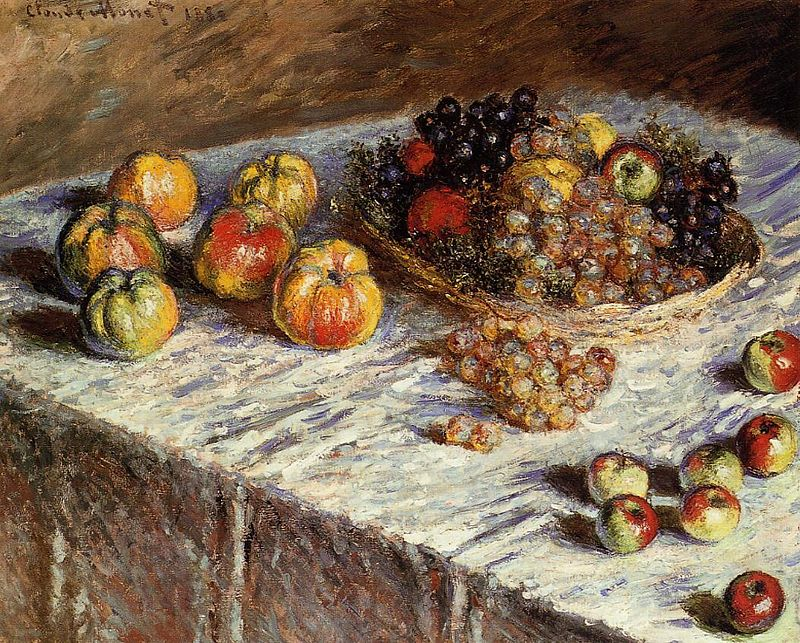
\includegraphics[width = .9\textwidth]{images/monetgrapes}\hfill\\ %QuinceCabbageMelonandCucumber.jpg}\hfil\\ % monetgrapes.jpg}\hfil\\
\begin{center}\emph{Still Life with Apples and Grapes} by Claude Monet (Public Domain) \end{center}}
%\begin{center}\emph{Quince, Cabbage, Melon and Cucumber} by Juan Sánchez Cotán (Public Domain) \end{center}}
%https://commons.wikimedia.org/wiki/File:Fra_Juan_Sánchez_Cotán_001.jpg
%replaced https://commons.wikimedia.org/wiki/File:Monet-Still-Life-with-Apples-and-Grapes-1880.jpg


\part{Prose}\label{part:prose}

\chapter{The Object-oriented Interface}\label{chapter:oop}
Matplotlib offers two interfaces: a MATLAB-style interface and the more cumbersome object-oriented interface. If you count yourself among the matplotlib-averse, you likely never had the stomach for object-oriented headaches. Still, we are using the object oriented interface because we can do more with this.

The MATLAB-style interface looks like the following. 

\pyfile{matlab-plot.py}

The object-oriented interface looks like this. 

\pyfile{oop-plot.py}


There is no such thing as a free lunch, so you will observe this interface requires more code to do the same exact thing. Its virtues will be more apparent later. Object-oriented programming (OOP) also requires some new vocabulary. OOP might be contrasted with procedural programming as another common method of programming. In procedural programming, the MATLAB-style interface being an example, the data and code are separate and the programmer creates procedures that operate on the program's data. OOP instead focuses on the creation of \emph{objects} which encapsulate both data and procedures. 

An object's data are called its \emph{attributes} and the procedures or functions are called \emph{methods}. In the previous code, we have figure and axes objects, making use of axes methods \code{plot()} and \code{set_title()}, both of which add data to the axes object in some sense, as we could extract the lines and title from \code{ax} with more code. Objects themselves are instances of a \emph{class}. So \code{ax} is an object and an instance of the Axes class. Classes can also branch into subclasses, meaning a particular kind of object might also belong to a more general class. A deeper knowledge is beyond our scope, but this establishes enough vocabulary for us to continue building an applied knowledge of matplotlib. Because \code{ax} contains its data, you can think of \code{set_title()} as changing \code{ax} and this helps make sense of the \code{get_title()} method, which simply returns the title belonging to \code{ax}. Having some understanding that these objects contain both procedures and data will be helpful in starting to make sense of intimidating programs or inscrutable documentation you might come across.  %These are Just as there is a \code{set_title()}

\section{Figure, Axes}

A plot requires a figure object and an axes object, typically defined as \code{fig} and \code{ax}. The figure object is the top level container. In many cases like in the above, you'll define it at the beginning of your code and never need to reference it again, as plotting is usually done with axes methods. A commonly used figure parameter is \code{figsize}, to which you can pass a sequence to alter the size of the figure. Both the figure and axes objects have a \code{facecolor} parameter which might help to illustrate the difference between the axes and figure. 


\pyfile{figparams.py}

\begin{center}
    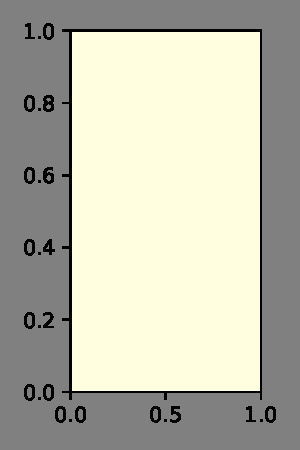
\includegraphics[width = .45\textwidth]{figures/proseplots/figparams.pdf}
\end{center}


The axes object, named \code{ax} by convention, gets more use in most programs. In place of \code{plt.plot()}, you'll use \code{ax.plot()}. Similary, \code{plt.hist()} is replaced with \code{ax.hist()} to create a histogram. If you have experience with the MATLAB interface, you might get reasonably far with the object-oriented style just replacing the \code{plt} prefix on your pyplot functions with \code{ax} to see if you have an equivalent axes method.

This wishful coding won't take you everywhere though. For example, \code{plt.xlim()} is replaced by \code{ax.set_xlim()} to set the $x$-axis view limits. To modfiy the title, \code{plt.title()} is replaced with \code{ax.set_title()} and there is \code{ax.get_title()} simply to get the title. The axes object also happens to have a \code{title} attribute, which is only used to access the title, similar to the \code{get_title()} method. Many matplotlib methods can be classified as \emph{getters} or \emph{setters} like for these title methods. The plot method and its logic is different. Later calls of \code{ax.plot()} don't overwrite earlier calls and there is not the same getter and setter form. There's a \code{plot()} method but no single \code{plot} attribute being mutated. Whatever has been plotted can be retrieved, or gotten (getter'd?), but it's more complicated and rarely necessary. Use the code below to see what happens with two calls of \code{plot()} and two calls of \code{set_title()}. The second print statement demonstrates that the second call of \code{set_title()} overwrites the title attribute, but a second plot does not nullify the first. 

%It's part of the object-oriented construction, which goes beyond our scope.
%\newpage

\pyfile{gettersetter.py}

\begin{center}
    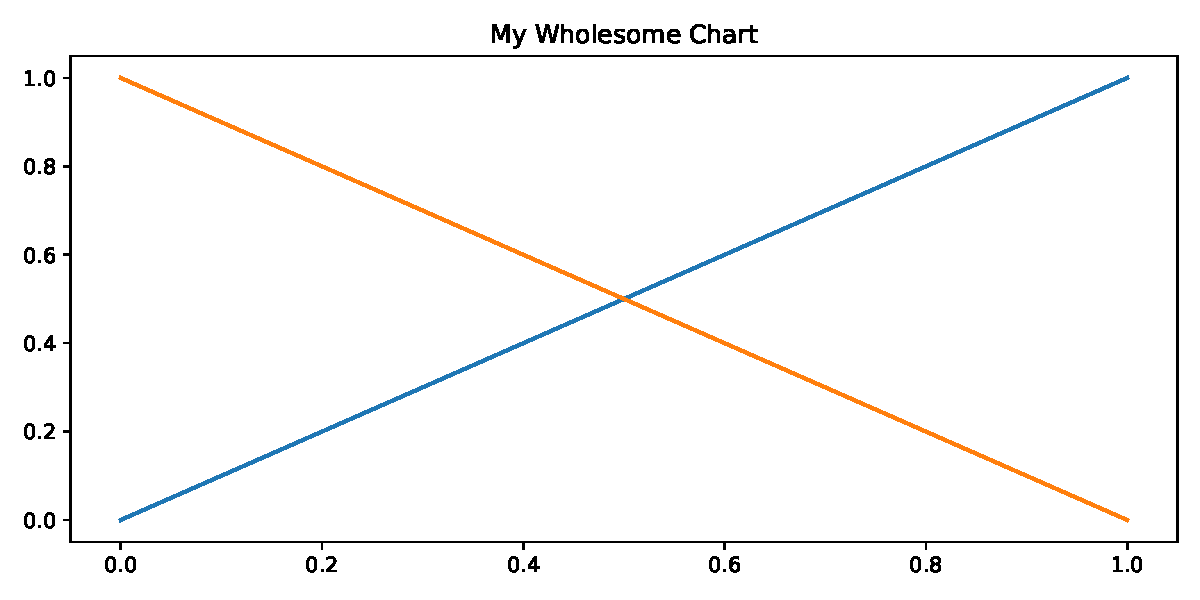
\includegraphics[width = .7\textwidth]{figures/proseplots/gettersetter.pdf}
\end{center}

Axes methods \code{set_xlim()} and \code{get_xlim()} behave just like \code{set_title()} and \code{get_title()}, but note there is no attribute simply accessible with \code{ax.xlim}, so the existence of getters and setters is the more fundamental pattern.\footnote{Getters and setters are thought of as old-fashioned. It's more Pythonic to access attributes directly, but matplotlib doesn't yet support this.}
%https://matplotlib.org/stable/tutorials/intermediate/artists.html?highlight=artist%20tutorial for old fashioned comment

\section{Mixing the Interfaces}

You can also mix the interfaces. Use \code{plt.gca()} to \emph{g}et the \emph{c}urrent \emph{a}xis. Use \code{plt.gcf()} to \emph{g}et the \emph{c}urrent \emph{f}igure.


\pyfile{chart.py}

\begin{center}
    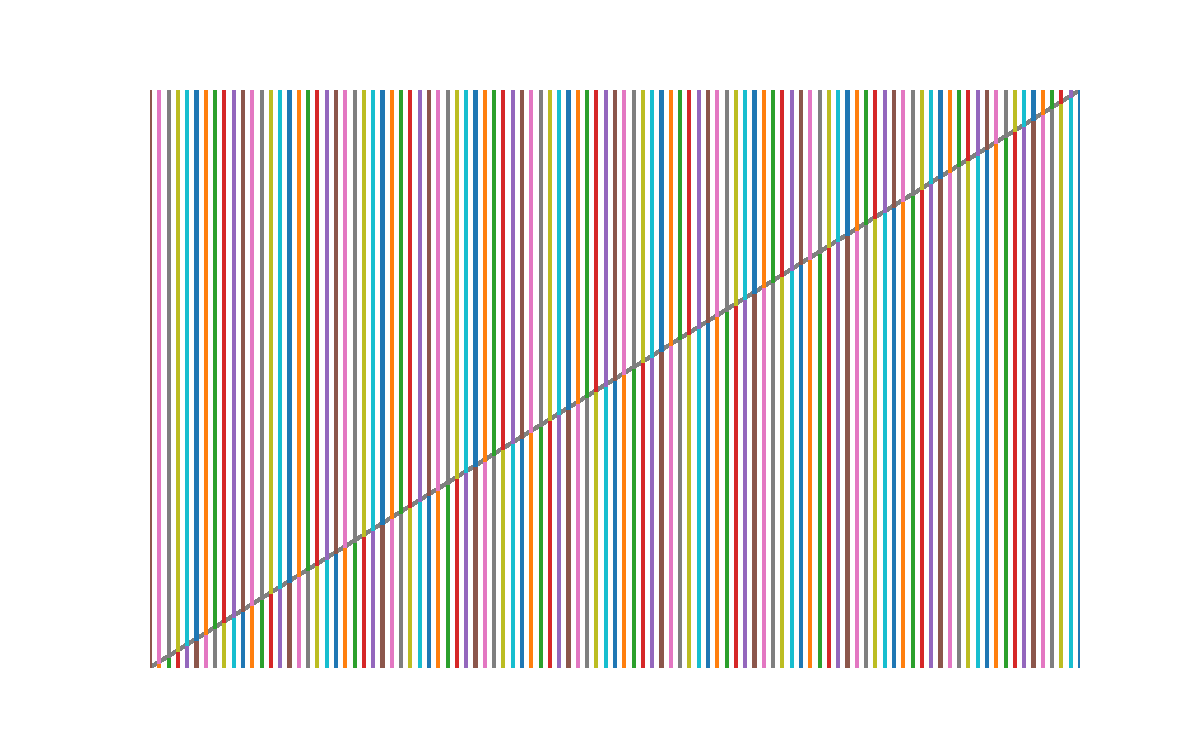
\includegraphics[width = .8\textwidth]{figures/proseplots/chart.pdf}
\end{center}


In the above, we started with MATLAB and then converted to object-oriented. We can also go in the opposite direction, though it's not always ideal, especially when working with subplots. Below, we start with our figure and axes objects, and then revert back to the MATLAB style with the \code{axvline()} functions (producing vertical lines across the axes), toggling off the axis lines and labels, and then saving the figure. This graph would appear unchanged if you replaced \code{plt.axvline()} with \code{ax.axvline()}, \code{plt.axis()} with \code{ax.axis()}, and \code{fig.savefig()} would do the same as \code{plt.savefig()}.

\pyfile{colorful.py}

%\vspace{-10pt}
\begin{figure}
    \centering
    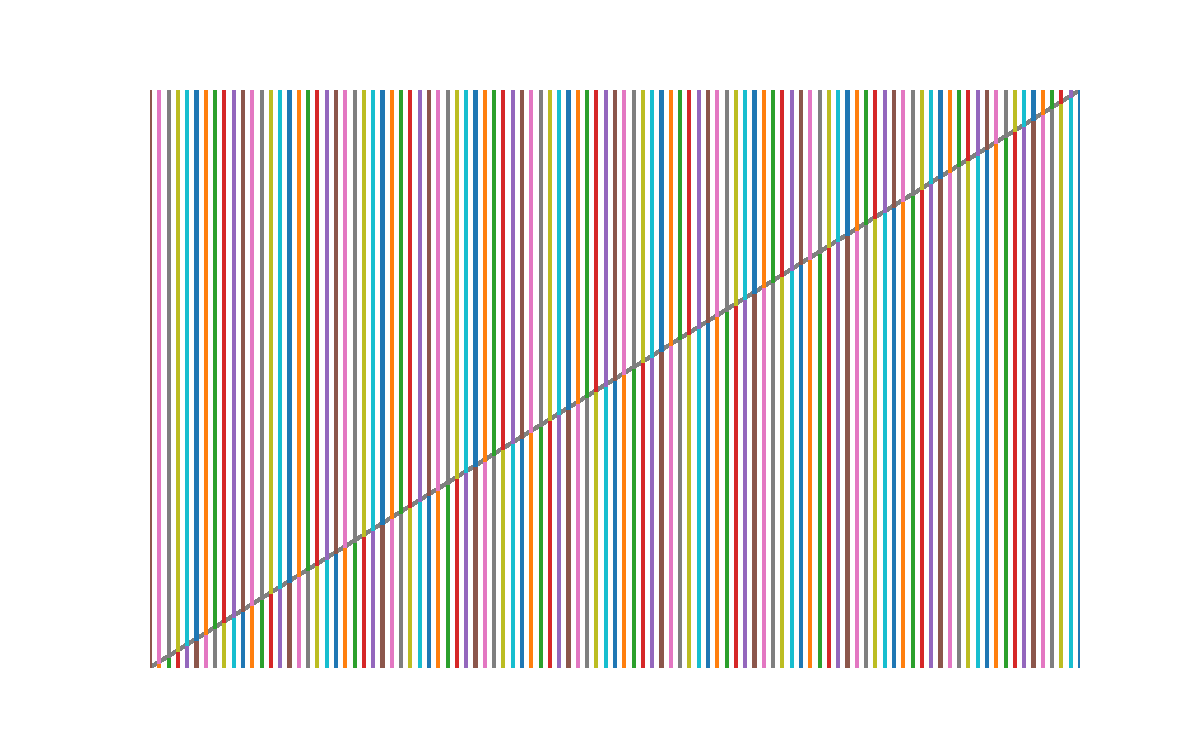
\includegraphics[width = .8\textwidth]{figures/proseplots/colorful.pdf}    %\caption{Caption}
    \label{fig:my_label}
\end{figure}


Matplotlib is also integrated into pandas, with a \code{plot()} method for both Series and DataFrame objects, among other functionalities. There is excellent documentation \link{https://pandas.pydata.org/pandas-docs/stable/user_guide/visualization.html}{available}.\footnote{\scalebox{.83}{https://pandas.pydata.org/pandas-docs/stable/user\_guide/visualization.html}} These plots can be mixed with the object-oriented interface. You can use a plot method and specify the appropriate axes object as an argument. Below we import the iris dataset and make a boxplot with a mix of axes methods and then pyplot functions. 

\pyfile{irisbox.py}

\begin{center}
    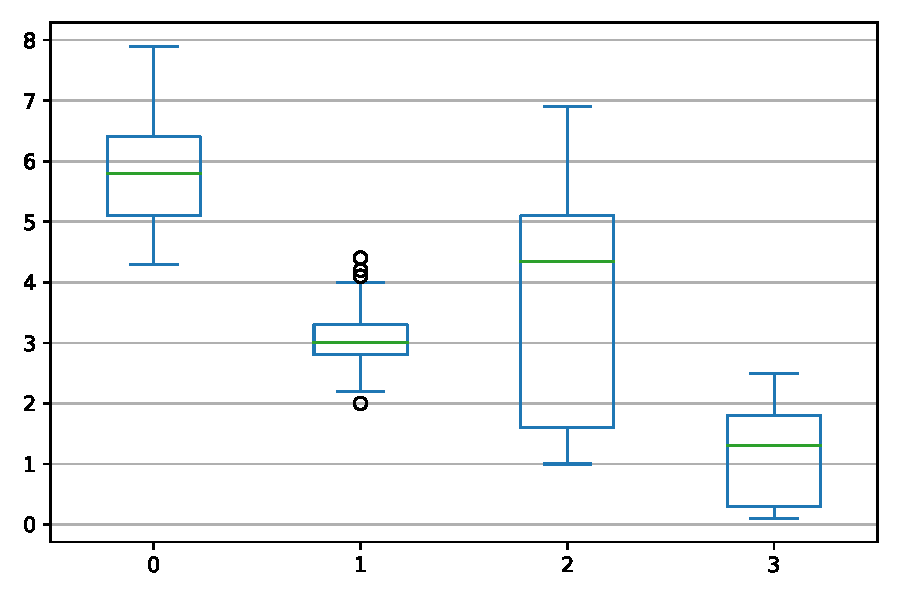
\includegraphics[width = .7\textwidth]{figures/proseplots/irisbox.pdf}
\end{center}

The above capability is handy, especially with subplots, where every subplot will have its own axes object as we will see later.  
%\link{https://matplotlib.org/stable/api/figure_api.html?highlight=figure\#module-matplotlib.figure}{test}



\chapter{Axes Appearance, Ticks, and Grids}\label{chapter:axes}
%This chapter focuses on the small things your plots swim in. If a line graph is a fish, the water is the 

\section{Axis Aspect and Limits}\label{sec:aspectLim}
The most basic plot is the empty plot. 

\pyfile{empty.py}

\begin{center}
    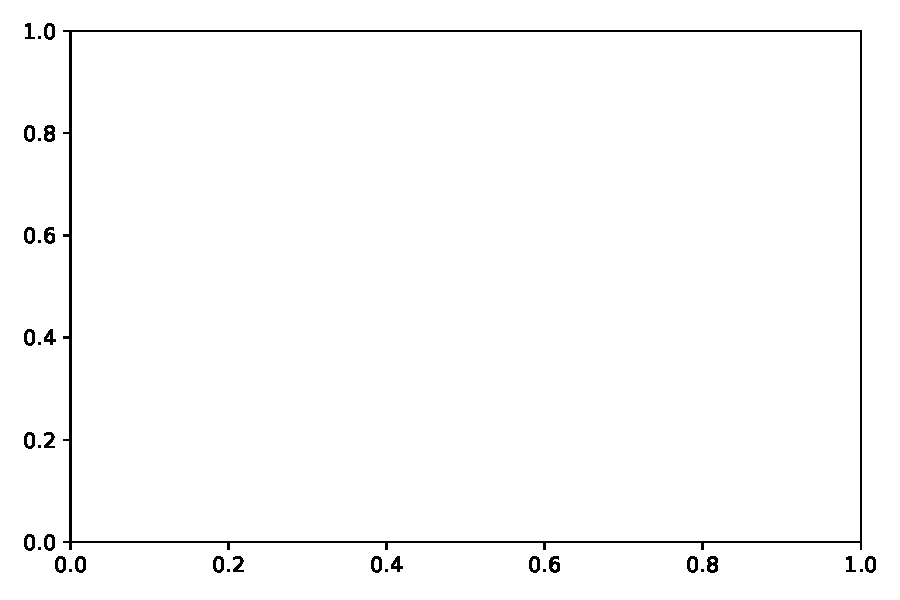
\includegraphics[width = .6\textwidth]{figures/proseplots/empty.pdf}
\end{center}


You'll notice this defaults to plotting the square region between data points (0,0) and (1,1). However, the plot is not square by default. That is to say the \emph{aspect} is not one, where the aspect is the ratio of height to width. This can be changed with the axes method \code{set_aspect()}. For equal scaling, use \code{ax.set_aspect('equal')} or \code{ax.set_aspect(1)}.

\pyfile{empty-square.py}

\begin{center}
    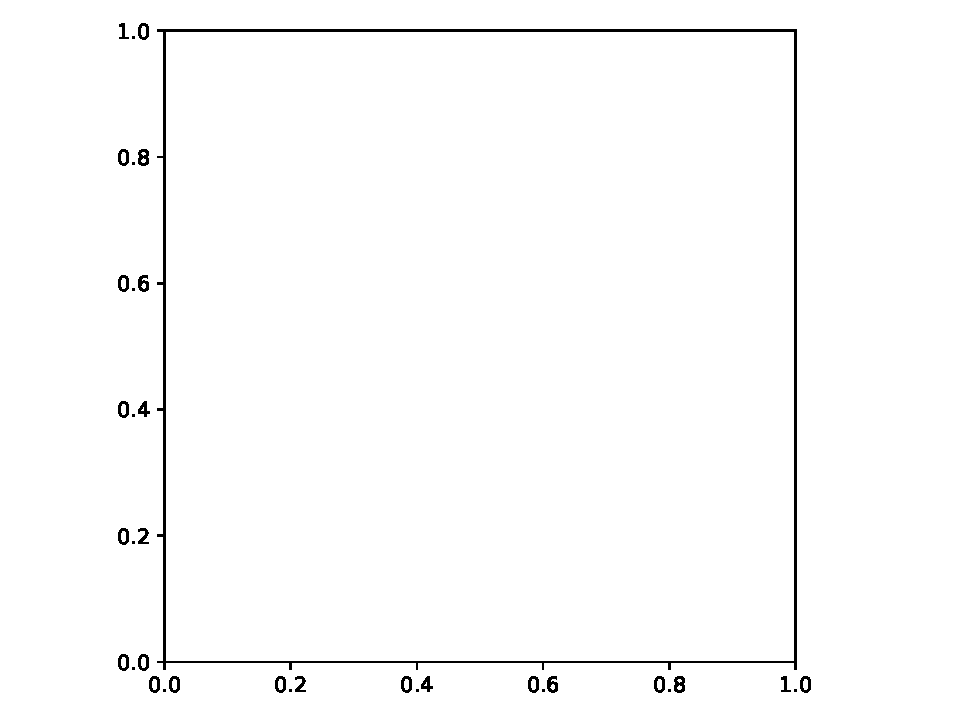
\includegraphics[width = .6\textwidth]{figures/proseplots/empty-square.pdf}
\end{center}

As we already covered in Chapter \ref{chapter:oop}, the $x$ and $y$ limits can be adjusted with axes methods \code{set_xlim()} and \code{set_ylim()}, taking a sequence for the minimum and maximum values. If you don't explicitly set the limits, matplotlib will set the limits automatically based on the data. You can retrieve those limits with the getter methods, \code{get_xlim()} and \code{get_ylim()}. 
The program below makes use of both methods. We plot a few lines, and after each plot call, matplotlib is quietly updating the axes limits. Using the \code{fill_between()} method, which creates a color fill in the defined region, the expanding limits are shown. The colors are chosen automatically by matplotlib because I haven't explicitly specified a color value. 

%I also use the \code{zorder} parameter, which specifies the ordering of the plotted objects. By default, text is plotted over lines and lines are plotted over other objects like the fill created by \code{fill_between()} (which belongs to a more general category called \emph{patches}). Within each of these three categories, objects created later in the program are plotted over previously created objects. \code{zorder} can be used to create a different ordering. Objects with a greater \code{zorder} value are ordered further to the front. Below, \code{zorder} is used to reverse the default order---the later fills are further to the back. 
% https://matplotlib.org/stable/api/_as_gen/matplotlib.axes.Axes.fill_between.html

\pyfile{expanding-lims.py}

\begin{center}
    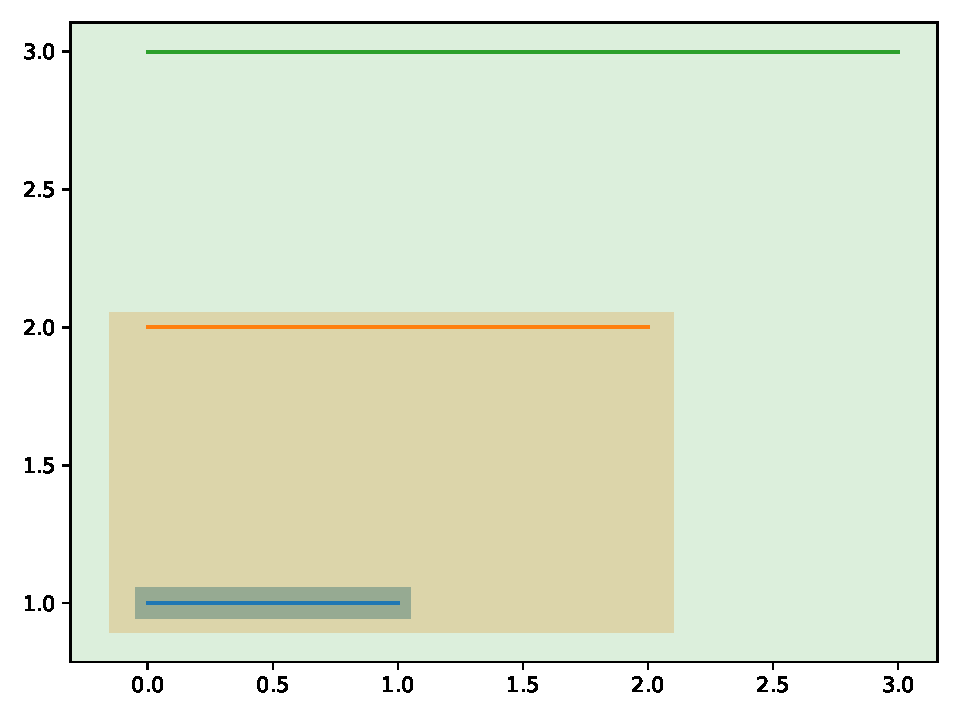
\includegraphics[width = .6\textwidth]{figures/proseplots/expanding-lims.pdf}
\end{center}

If your axes limits are too restrictive, plot elements will be cut off. If you want your plot element to break past the end of the axes, spilling into the outer figure space, you can change this by setting \code{clip_on = False} in the appropriate method. Below, we create two circles with \code{ax.plot()} and set restrictive $x$-axis limits. The first circle, in blue, would extend further to the left if the limits were more generous. By default, it is clipped so we only see half of a circle. In the next call to \code{ax.plot()}, we create an orange circle and toggle \code{clip_on = False}. As a result, the circle extends to the right of the axes limits into the remaining figure space. 

\pyfile{circle-clip.py}

\begin{center}
    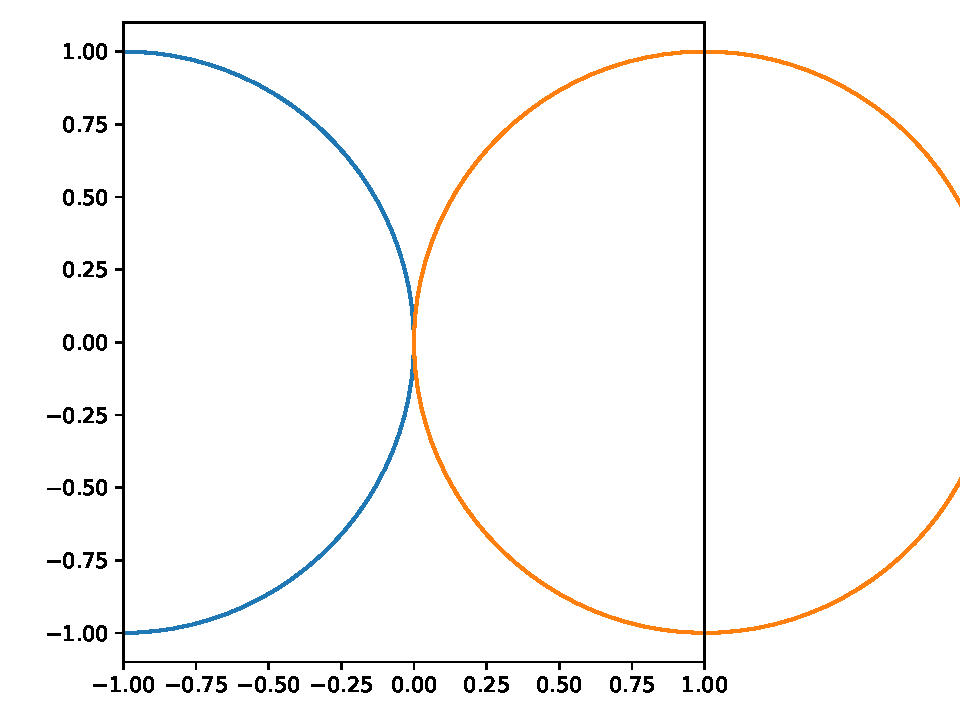
\includegraphics[width = .7\textwidth]{figures/proseplots/circle-clip.pdf}
\end{center}

\section{Axis Lines and Spines}\label{sec:axisSpines}

You might be used to plots that aren't surrounded by a box. Those enclosing lines, included by default, are called the \emph{spines}. The default might also be jarring if you're used to the typical $x$- and $y$-axis lines at $y=0$ and $x=0$, like in most math textbook plots. In this section we'll cover how to modify these. 

First, you might just eliminate everything with \code{ax.axis('off')}. We saw \code{plt.axis('off)} used similarly in Chapter \ref{chapter:oop} with a program that alternated between pyplot functions and the object-oriented approach. Below is a simple plot, empty but for a title, that becomes even emptier by eliminating the axis lines and labels. For reference, on the right is the same plot if \code{ax.axis('off')} were excluded from the program. 


\pyfile{no-axis.py}

\begin{center}
    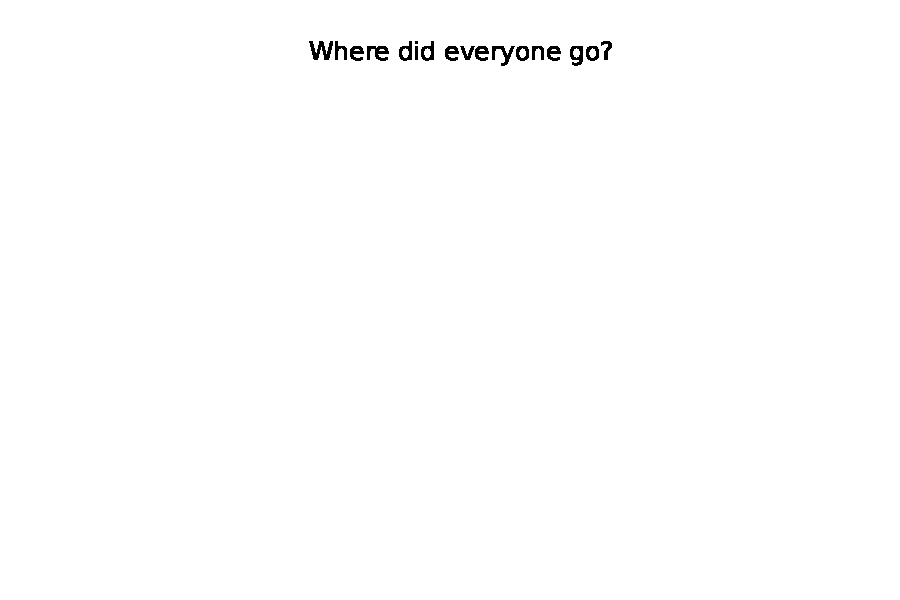
\includegraphics[width = .45\textwidth]{figures/proseplots/no-axis.pdf}   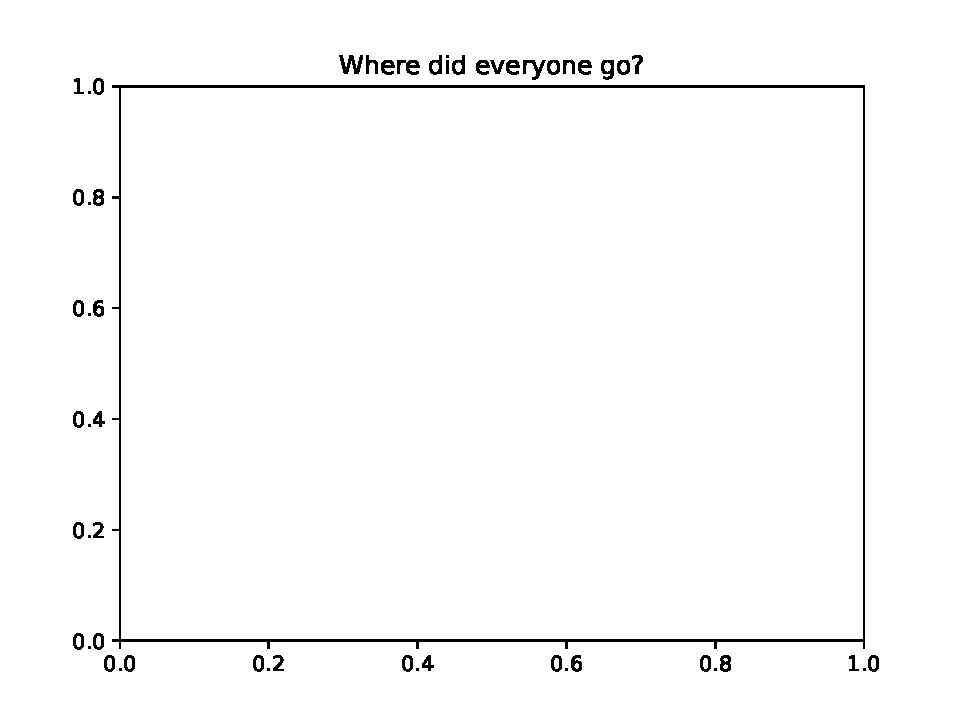
\includegraphics[width = .45\textwidth]{figures/proseplots/yes-axis.pdf}  %\caption{Caption}
\end{center}


Next, we can access and modify specific spines through \code{ax.spines}, which returns an \code{OrderedDict}. Access a specific spine using the appropriate key: \code{"left"}, \code{"right"}, \code{"top"}, or \code{"bottom"}.
A spine can be toggled on or off by passing the appropriate boolean value to \code{set_visible()}.

\pyfile{spine-vis.py}

\vspace{-0.2cm}
\begin{center}
    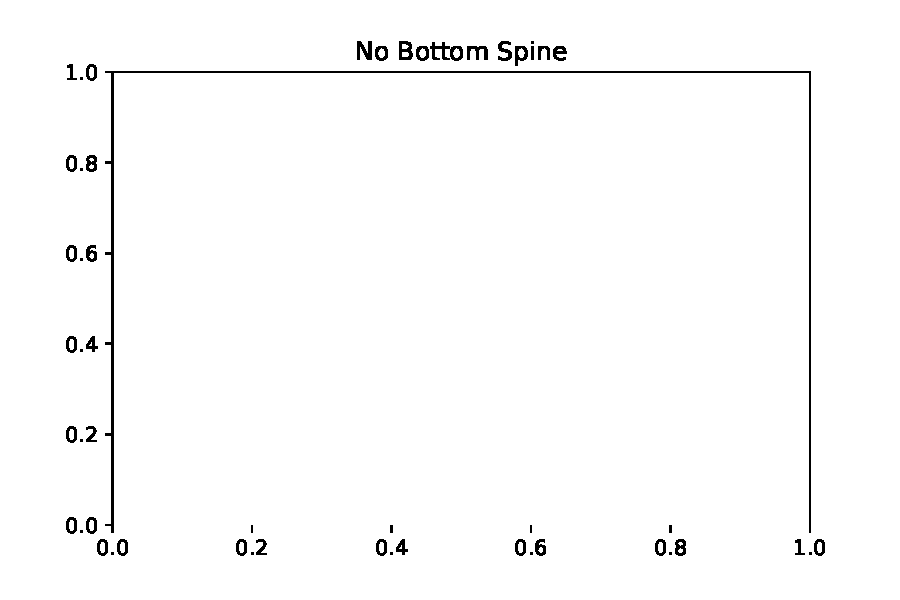
\includegraphics[width = 0.48\textwidth]{figures/proseplots/spine-vis-bottom.pdf} 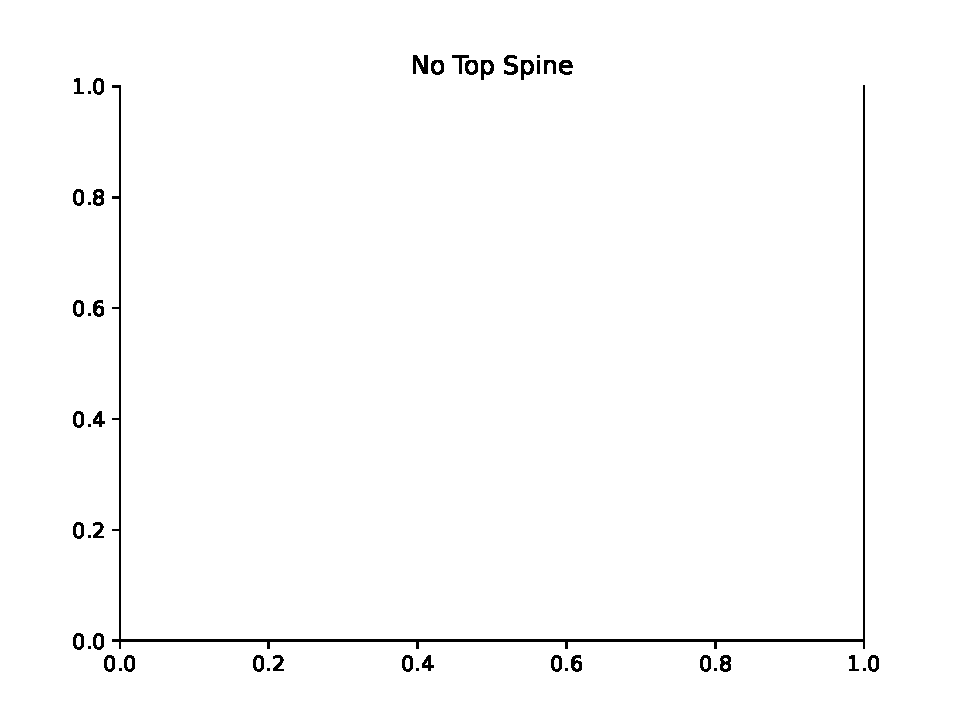
\includegraphics[width = 0.48\textwidth]{figures/proseplots/spine-vis-top.pdf}
    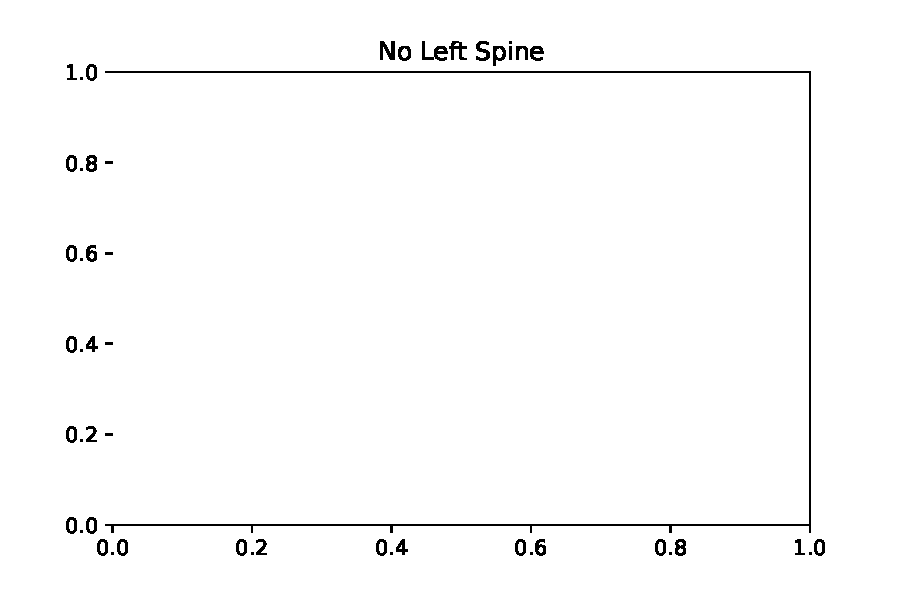
\includegraphics[width = 0.48\textwidth]{figures/proseplots/spine-vis-left} 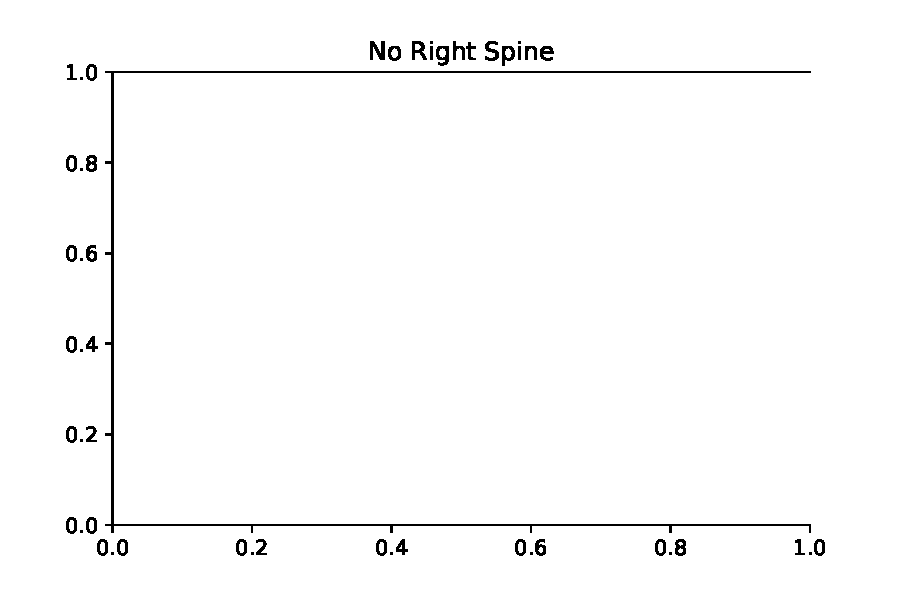
\includegraphics[width = 0.48\textwidth]{figures/proseplots/spine-vis-right.pdf}
\end{center}

Other spine modifications might be their width and color. Again, we access a particular spine and then make use of setter methods, \code{set_color} and \code{set_linewidth} in particular. 

\pyfile{thick-spines.py}
\begin{center}
    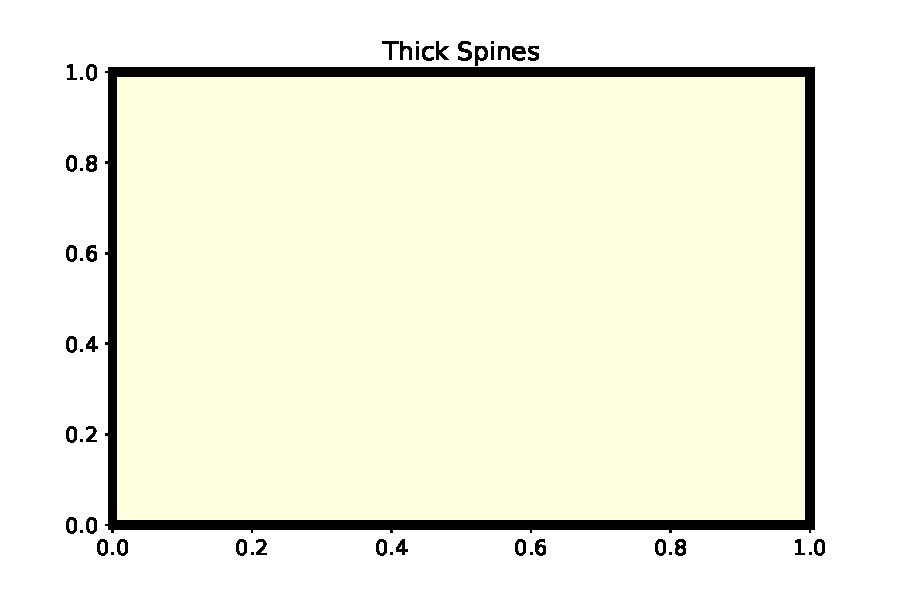
\includegraphics[width = .7\textwidth]{figures/proseplots/thick-spines.pdf}
\end{center}

It's easy to get this far imagining that spines are simply the pieces of the box enclosing your plot. But they don't have to enclose the plot if we alter them with the \code{set_position} method. Below, we set the bottom spine to be along the usual $x$-axis and the left spine to be along the usual $y$-axis by passing \code{'zero'} to \code{set_position}. The right and top spines are removed. 

\pyfile{zero-spines.py}

\begin{center}
    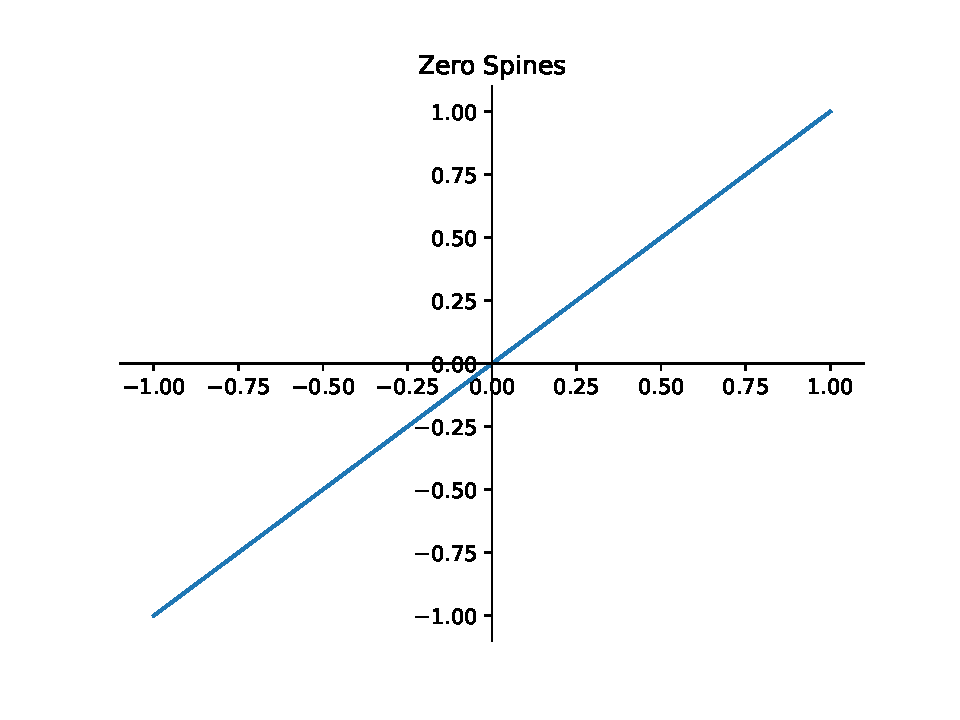
\includegraphics[width = .7\textwidth]{figures/proseplots/zero-spines.pdf}
\end{center}

We can go a step further and add arrows at the ends of our axis lines with some clever plotting. 
%https://matplotlib.org/stable/gallery/ticks_and_spines/centered_spines_with_arrows.html#sphx-glr-gallery-ticks-and-spines-centered-spines-with-arrows-py

\pyfile{arrow-axes.py}

\begin{center}
    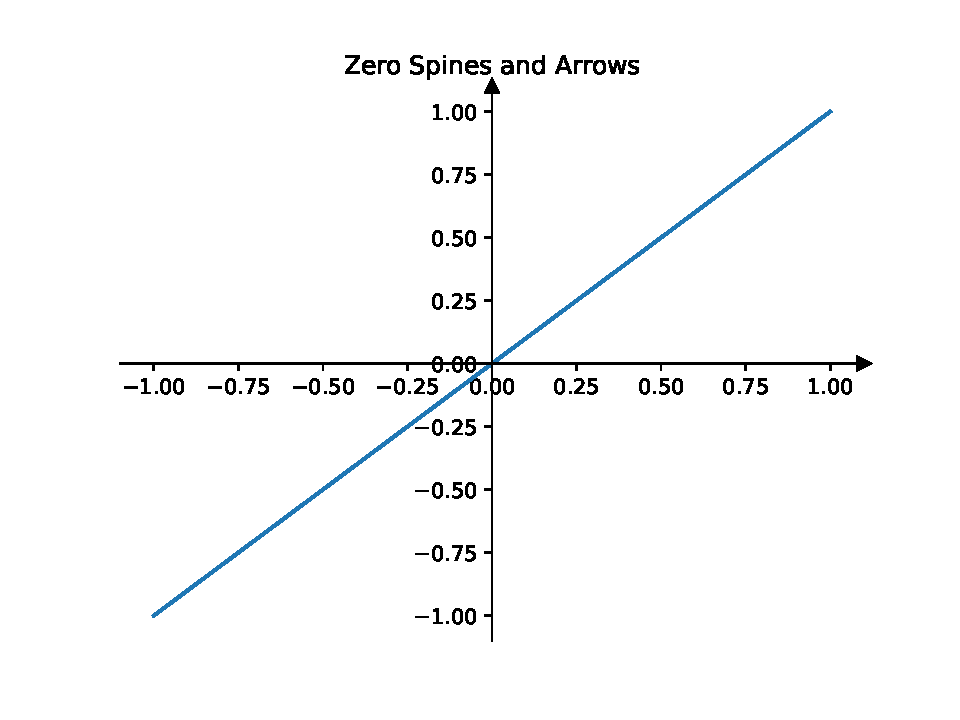
\includegraphics[width = .7\textwidth]{figures/proseplots/arrow-axes.pdf}
\end{center}

The tick labels do clutter the graph above. This can be solved after we cover Section \ref{sec:ticks}. \cite{knaflic2015storytelling} recommends removing the top and right spines as part of the imperative to declutter and remove unnecessary chart border. I think it is arguable. I'm used to default spines enclosing the data. Removing them can seem untidy, like the plot guts might spill out onto the page, or as if the plot is now vulnerable to intruders without any fencing. Arrows on axis lines subtly prod the reader to imagine what happens outside of the plotted region. I don't like that if, for example, I don't want to create the impression that a linear trend in a time series graph will continue into the future. 
% I also like that borders might subtly lessen your tendency to imagine the trend continuing beyond the axis limits. 
% see George Cumberland and William blake thoughts on outline
% page 33 from Blake biog Eternity's Sunrise


\section{Ticks}\label{sec:ticks}
%% Add something about ticks on the right for time series??

The important axes methods for ticks are \code{set_xticks}, \code{set_xticklabels}, and the natural $y$-axis counterparts. One may also use the general \code{set_ticks} and \code{set_ticklabels} with \code{ax.xaxis} or \code{ax.yaxis}---as axis (not axes) methods. These are demonstrated below, taking an array of tick locations and then the corresponding labels. I use \LaTeX strings to label the ticks. Here, that allows for a prettier $y$-axis, using fractions instead of decimals for tick labels. And on the $x$-axis, we can give a proper label of $\pi$ at $x = \pi$.

\pyfile{ticks1.py}

\begin{center}
    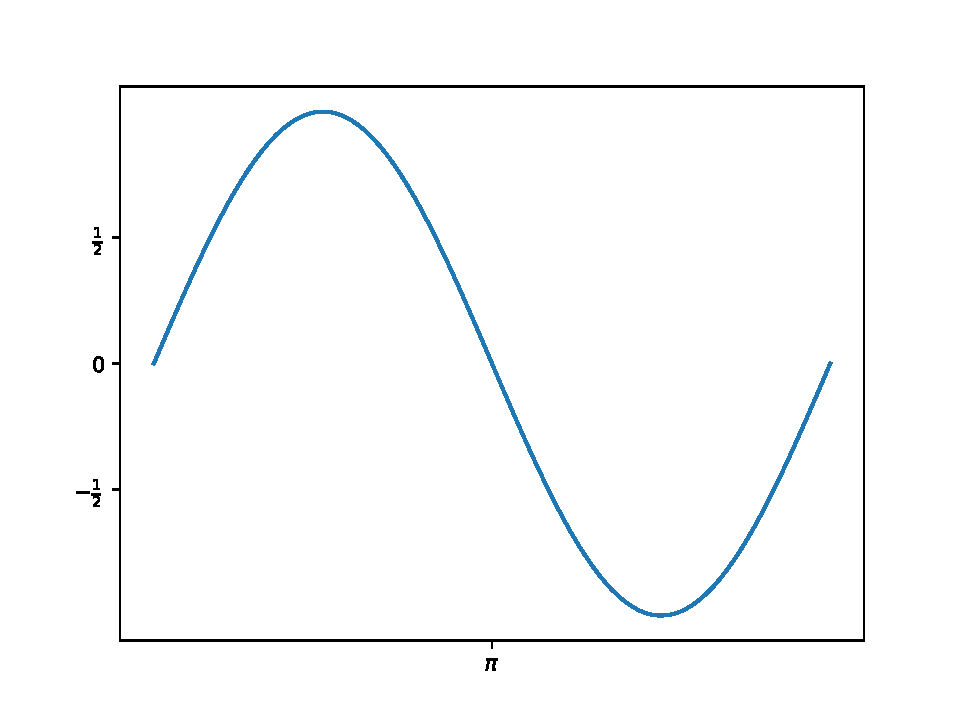
\includegraphics[width = .75\textwidth]{figures/proseplots/ticks1.pdf}
\end{center}

To remove the ticks entirely, simply pass an empty array to \code{set_ticks()}. To customize the appearance of your axis ticks and the labels, use the \code{set_tick_params} axis method. Parameters include \code{direction}, \code{width}, \code{length}, \code{color}, \code{pad}, \code{rotation}, \code{labelsize}, \code{labelcolor}

Imagine a measuring ruler, with ticks for every inch and smaller ticks at smaller intervals. So far our ticks have lacked that level of depth, but in fact we can work with two tick levels in matplotlib, major and minor ticks. Minor ticks are not shown by default. 

To start exploring these further customizations, you'll need to import additional formatters and or locators. For the below, you must import \code{MultipleLocator}, running \code{from matplotlib.ticker import MultipleLocator}.

\pyfile{tall-ballers.py}

\begin{center}
    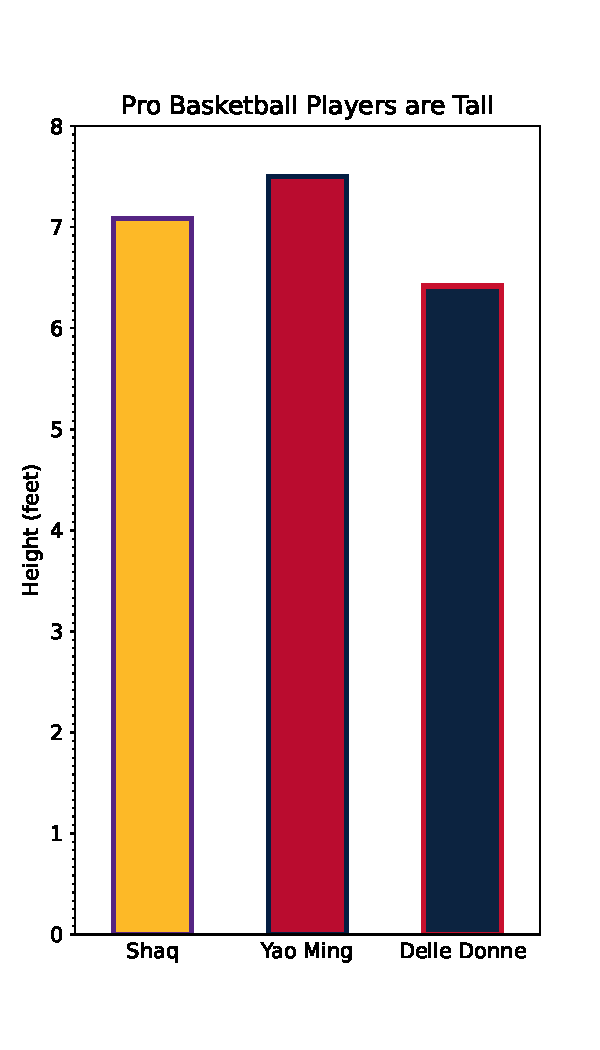
\includegraphics[width = .6\textwidth]{figures/proseplots/tall-ballers.pdf}
\end{center}

Major ticks can easily be set with \code{set_ticks} and its variants. Still, \code{MultipleLocator} and other locators are useful for setting major ticks without fooling with the details of the axes limits. 

With a function like $\sin x$, ticks might most naturally be placed at multiples of $\pi$. This can be accomplished by the below.

\pyfile{mult-locator.py}
\begin{center}
    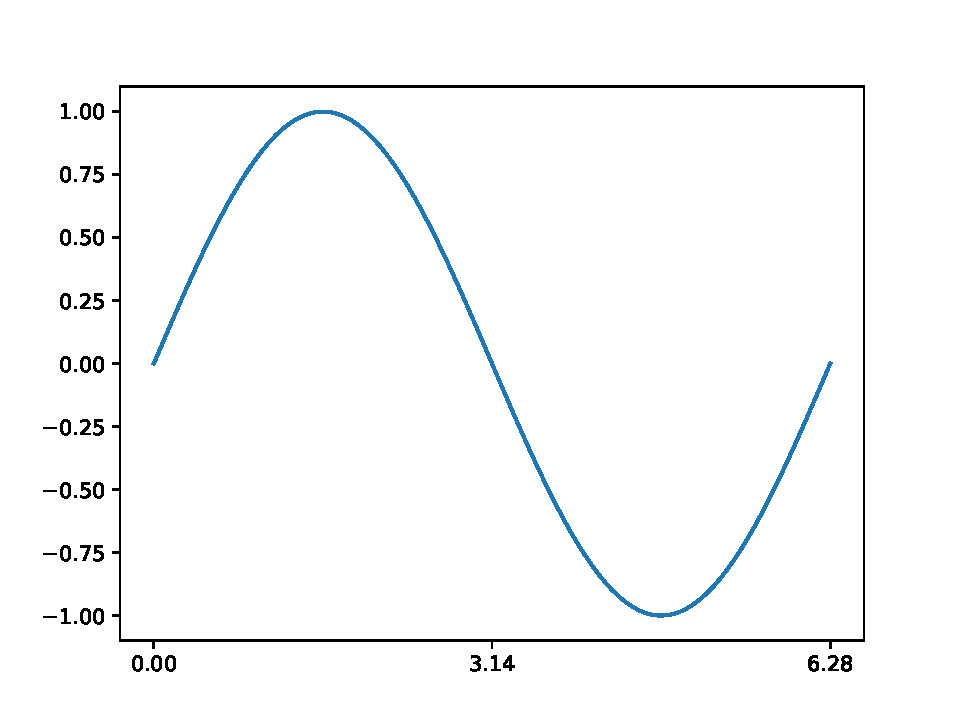
\includegraphics[width = .6\textwidth]{figures/proseplots/mult-locator.pdf}
\end{center}


It's true you could avoid the complication of locator classes by just using \code{ax.set_xticks([0, np.pi, 2*np.pi])}. For a plot this simple, do that. Suppose, you put ticks up to $3\pi$ though. Then you've extended the $x$-axis limit of the plot past your data. So you need to know your data to make the right tick adjustments by hand. If you'll be using the same code with different datasets, it'll be easier to use the details-free \code{MultipleLocator} and you can still rely on limit defaults or adjust them independently. 

Next, you might want to change the positioning of the ticks. By default $x$-axis ticks are on the bottom and $y$-axis ticks are on the left. You can modify these positions with axis methods. In time series data, for example, you might prefer to have the $y$-axis ticks on the right. Time marches on to the right and placing your ticks on the right can help emphasize that movement. This can be done with \code{set_ticks_position('right')} or the more concise \code{tick_right()}. The latter also accepts arguments of \code{'left'}, \code{'bottom'}, and \code{'top'}. Each has an abbreviated method like \code{tick_left()}. 

\pyfile{tick-right.py}

\begin{center}
    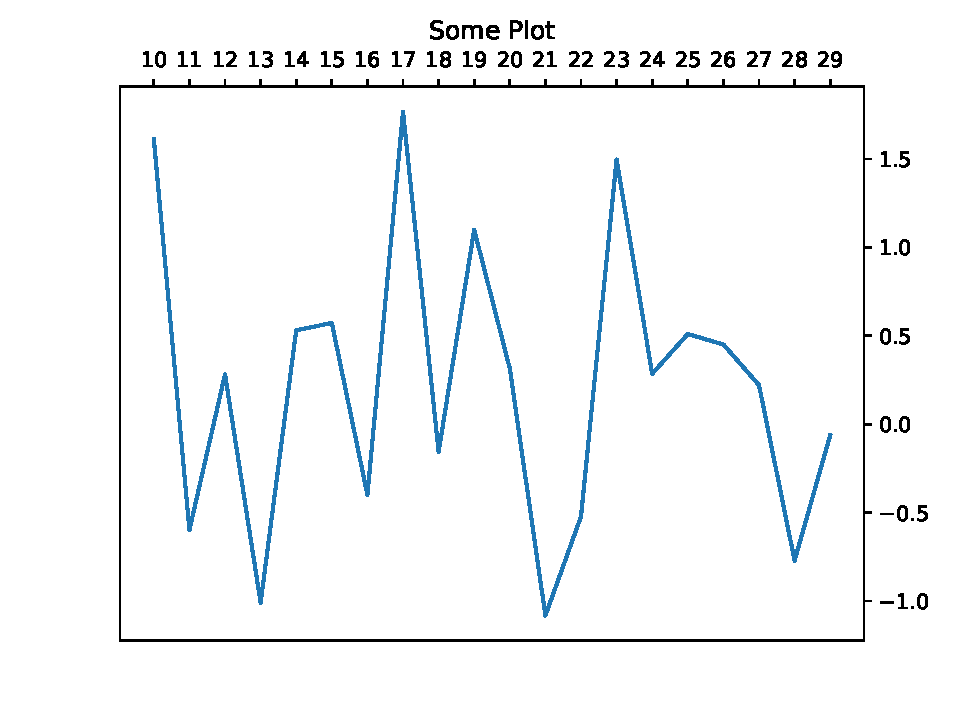
\includegraphics[width = .7\textwidth]{figures/proseplots/tick-right.pdf}
\end{center}

\section{Grids}

Including gridlines in a plot is generally discouraged (\cite{knaflic2015storytelling}, \cite{schwabish2021better}). It's clutter that won't spark joy. Perhaps we could stop here, with the instruction to run \code{ax.grid(False)} as in the code below (or rely on a style, like the default, that does this automatically).

\pyfile{grid-false.py}

\begin{center}
    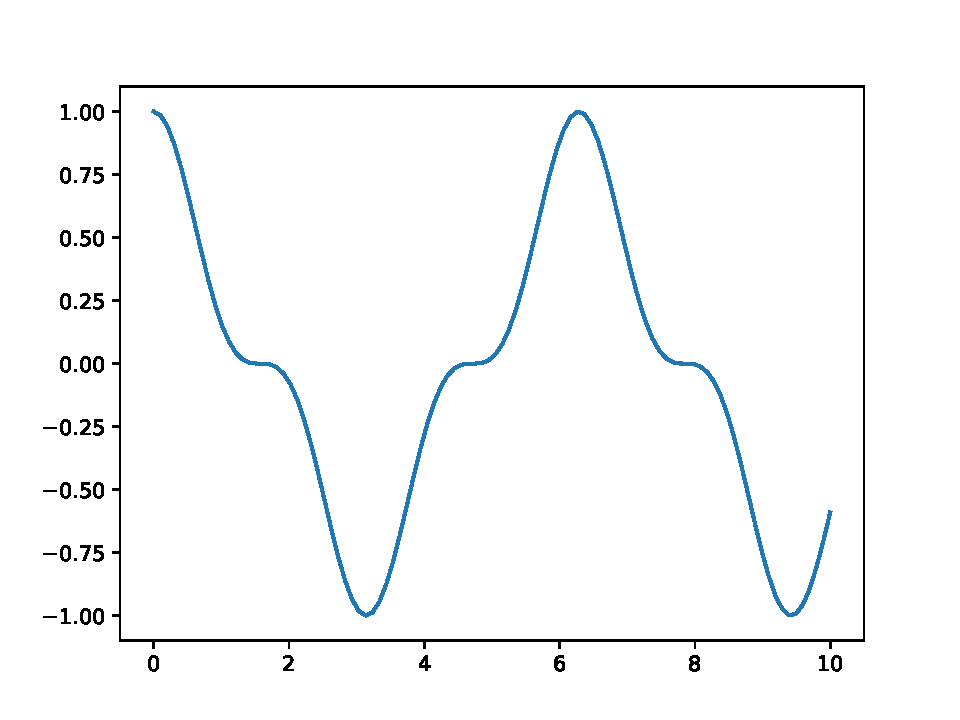
\includegraphics[width = .8\textwidth]{figures/proseplots/grid-false.pdf}
\end{center}

\noindent This does seem preferable to the following, but it's hardly an abomination. 

\pyfile{grid-true.py}

\begin{center}
    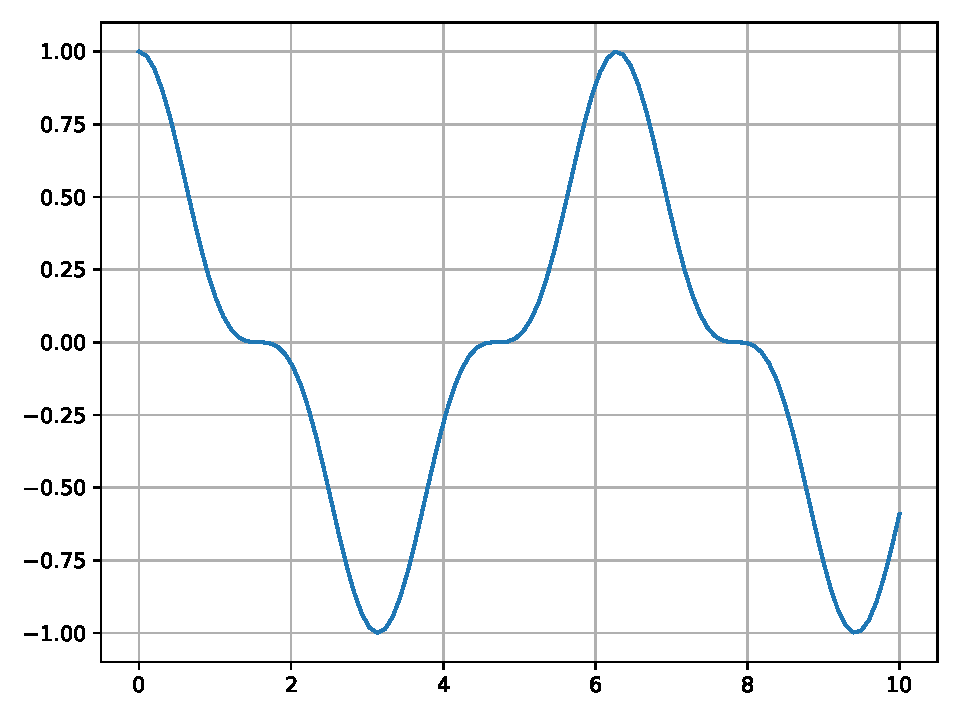
\includegraphics[width = .8\textwidth]{figures/proseplots/grid-true.pdf}
\end{center}

As a compromise, you might include gridlines for a single axis. If you want to emphasize that there is a slight trend in the data, then $y$-axis gridlines can help bring that pattern to the eye. Below we plot plots with and without a line of best fit and gridlines. Axis gridlines can be toggled independently by using \code{ax.xaxis.grid()} and \code{ax.yaxis.grid()}. 

\pyfile{y-grid-false.py}

\pyfile{y-grid-true.py}

\begin{center}
    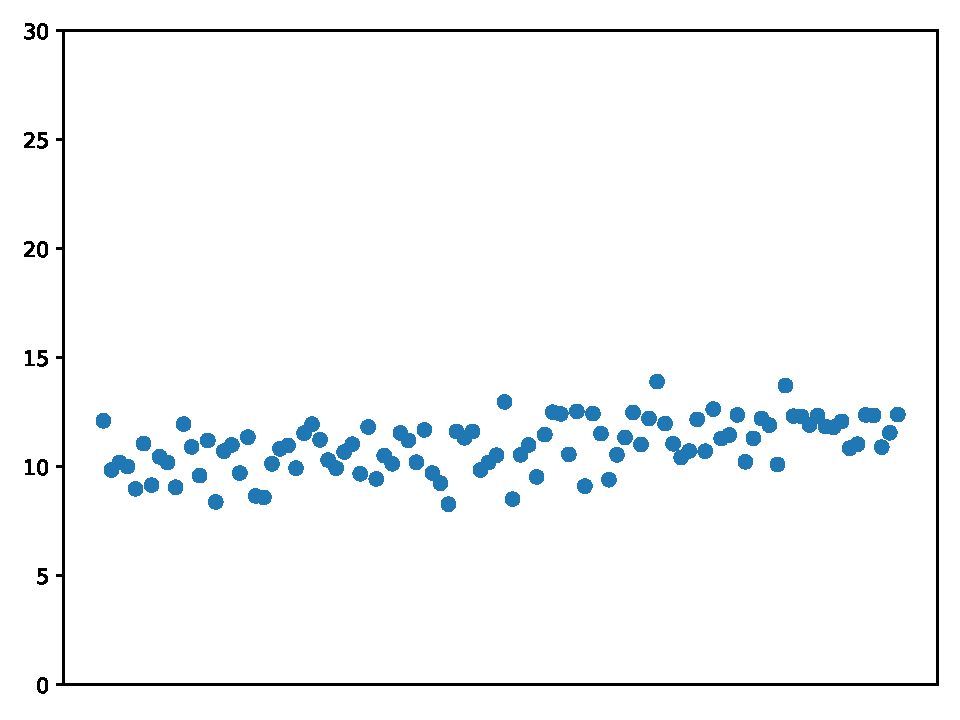
\includegraphics[width = .48\textwidth]{figures/proseplots/y-grid-false.pdf}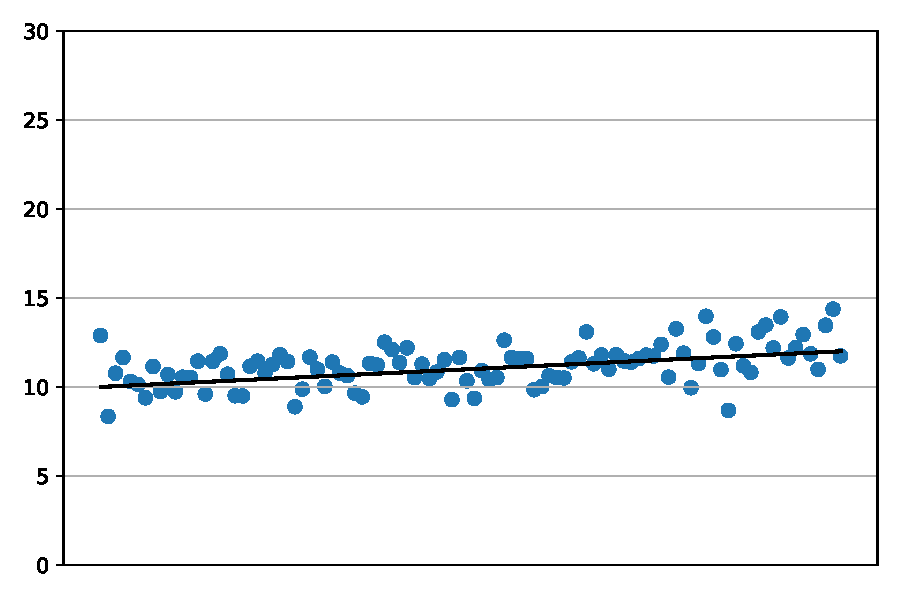
\includegraphics[width = .48\textwidth]{figures/proseplots/y-grid-true.pdf}
\end{center}



What we learned previously about locating ticks in Section \ref{sec:ticks} can be reapplied here, as seen in the examples further below. The location of gridlines and ticks can be set by the \code{set_major_locator()} and \code{set_minor_locator()} methods. \code{ax.grid()} is used to display the gridlines, but note it features a parameter \code{which}. The default value of \code{which} is \code{'major'}. To include minor gridlines, those minor ticks must be explicitly created (at least in the default style) and then the gridlines must be toggled on with \code{ax.grid(True, which = 'minor')} or for a single axis with \code{ax.xaxis.grid(True, which = 'minor')} for example. 


\pyfile{grids-auto.py}

\begin{center}
    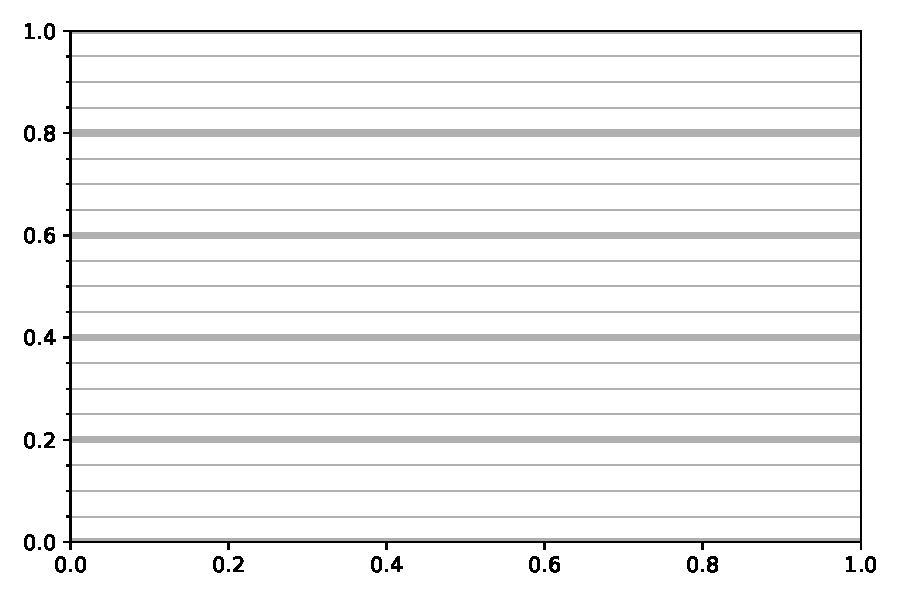
\includegraphics[width = .8\textwidth]{figures/proseplots/grids-auto.pdf}
\end{center}

\pyfile{grids-multi.py}

\begin{center}
    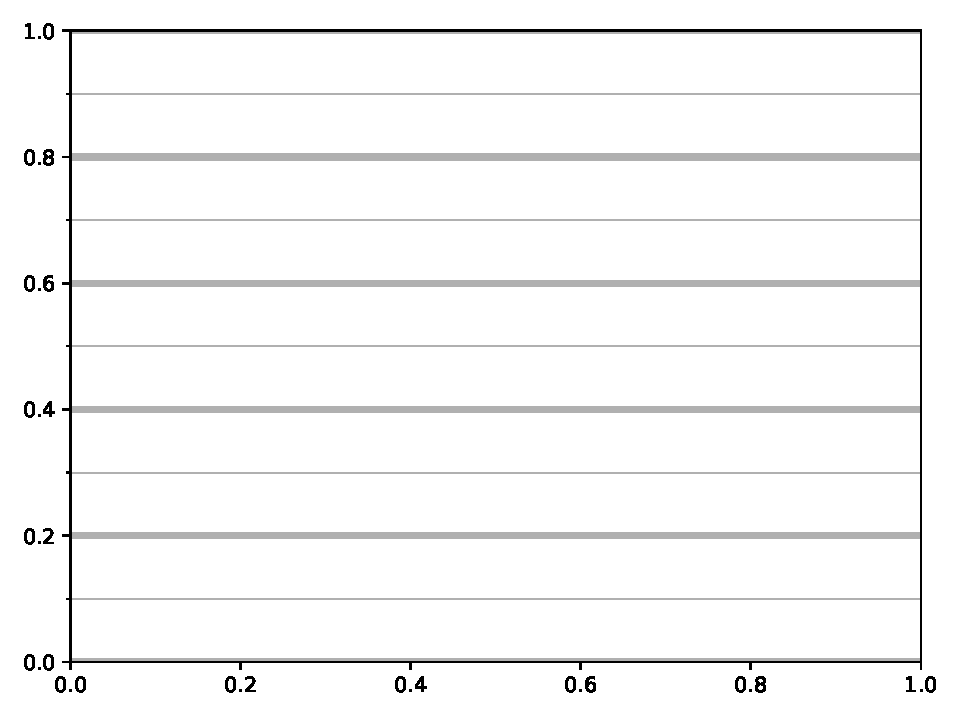
\includegraphics[width = .8\textwidth]{figures/proseplots/grids-multi.pdf}
\end{center}



%\section{Coordinates}

\chapter{Plot Elements and Coordinate Systems}\label{chapter:elements}
\chaptermark{Elements and Coord. Sys.}
%https://matplotlib.org/stable/tutorials/intermediate/artists.html#sphx-glr-tutorials-intermediate-artists-py

This chapter can be skipped by the reader in a hurry. I include it to establish some vocabulary about the basic plot elements and then discuss the different coordinate systems that can be used within a single plot---not polar vs. Cartesian coordinates but data coordinates vs. figure coordinates, for example. Coordinate systems do come up repeatedly in future chapters.


\section{Primitives and Containers}

Once you have a your figure and axis objects, you'll want to add actual plot elements to them, lines for a line chart, bars for a bar chart, annotations, etc. We already did that in Chapter \ref{chapter:oop}, creating line plots. In matplotlib, these elements belong to the Artist class, it being a very general base class. Artists objects are basically the water you've been swimming in this whole time---you just might not have noticed it. Artist objects can be either primitives or containers. Containers include background items like the figure and axes objects. Primitives are the meat of the plot, like the line created by a call to \code{ax.plot()}. Important primitive Artist objects include Line2D, Patches, and Text. 

\pyfile{artists.py}

\begin{center}
    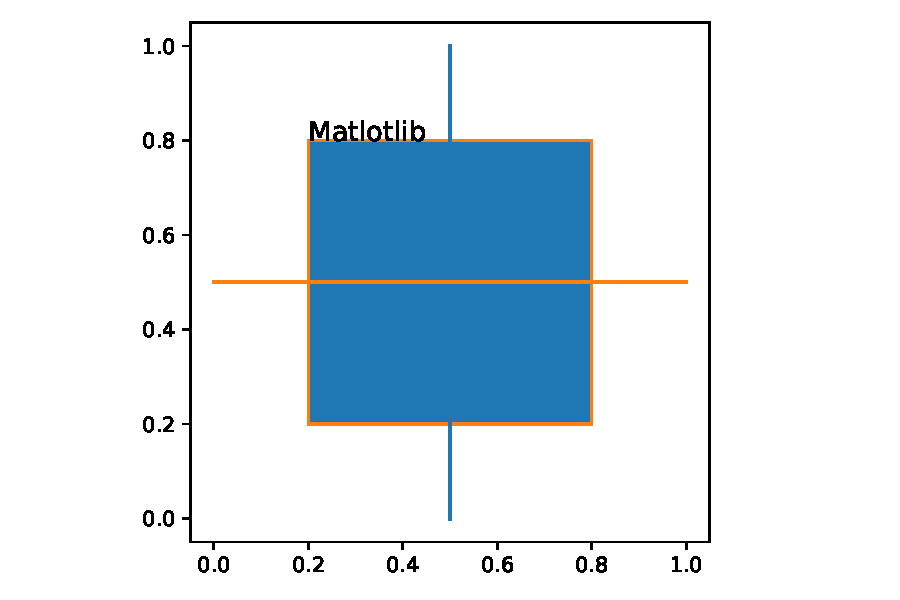
\includegraphics[width = .7\textwidth]{figures/proseplots/artists.pdf}
\end{center}


What might be unusual in the above is that we don't simply run \code{ax.plot(x, y)}. Instead we actually assign the plot call to a variable, \code{line, = ax.plot(x,y)}. Usually, this isn't necessary, but this allows us to reference the same object later in the program. The plot method creates a tuple of Line2D objects. In this case, that tuple contains only one item and it is assigned to the variable \code{line}. 

Now that we have the object as \code{line}, we can get properties or make changes. You can obtain the color with the \code{get_color()} method or change it with \code{set_color()}. You can even remove the plot element with \code{line.remove()}. These are all niche uses. However, we will later make use of \code{remove()} when iteratively centering text. We'll also use the \code{get_window_extent()} artist method frequently to help space objects in the plot. 


\subsection{Ordering with \code{zorder}}
% https://matplotlib.org/stable/gallery/misc/zorder_demo.html

\subsubsection{Default Ordering}
By default, text is plotted over lines and lines are plotted over patches, like the fill created by \code{fill_between()}. Within each of these three categories, objects created later in the program are plotted over previously created objects. The \code{zorder} parameter can be used to create a different ordering. Objects with a greater \code{zorder} value are ordered further to the front. 

First, we create and plot without specifying the \code{zorder} for any object to observe default behavior. We also print the zorder for each object using \code{get_zorder()}. Text has a \code{zorder} of 3, lines have a \code{zorder} of 2, and each patch object will have \code{zorder = 1}. Note \code{patch1} and \code{patch2} have the same \code{zorder}, but the red \code{patch2} is added later in the program so it is plotted over the green \code{patch1}, being as if \code{patch1} has a lower \code{zorder}. 


\pyfile{default-z.py}

\begin{center}
    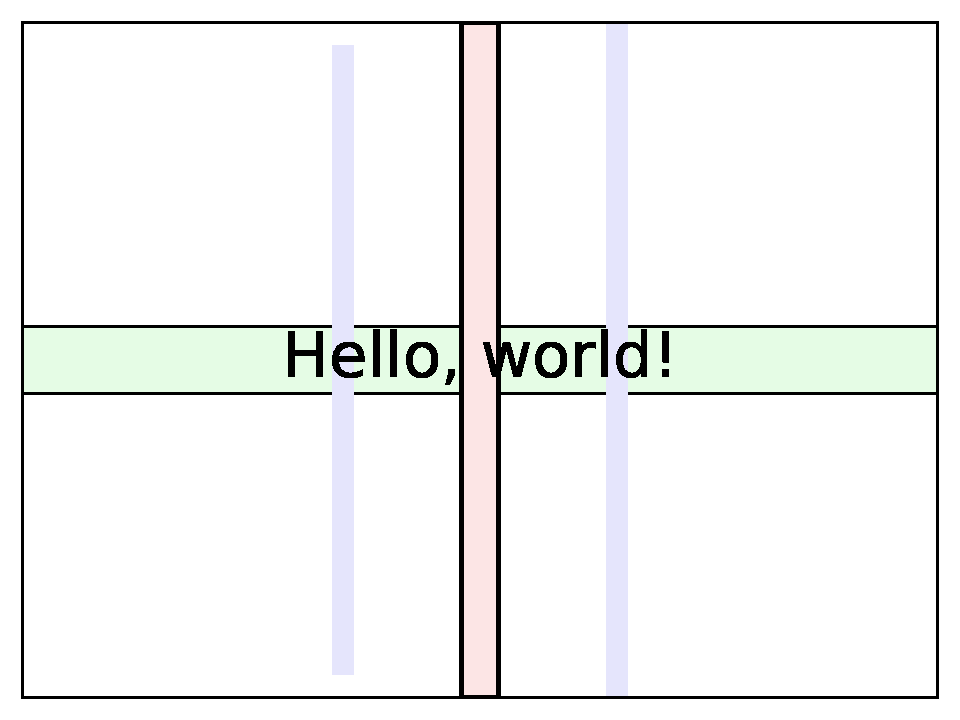
\includegraphics[width = .7\textwidth]{figures/proseplots/default-z.pdf}
\end{center}

\subsubsection{Custom Ordering}

Then, we reverse the ordering.

\pyfile{reverse-z.py}

\begin{center}
    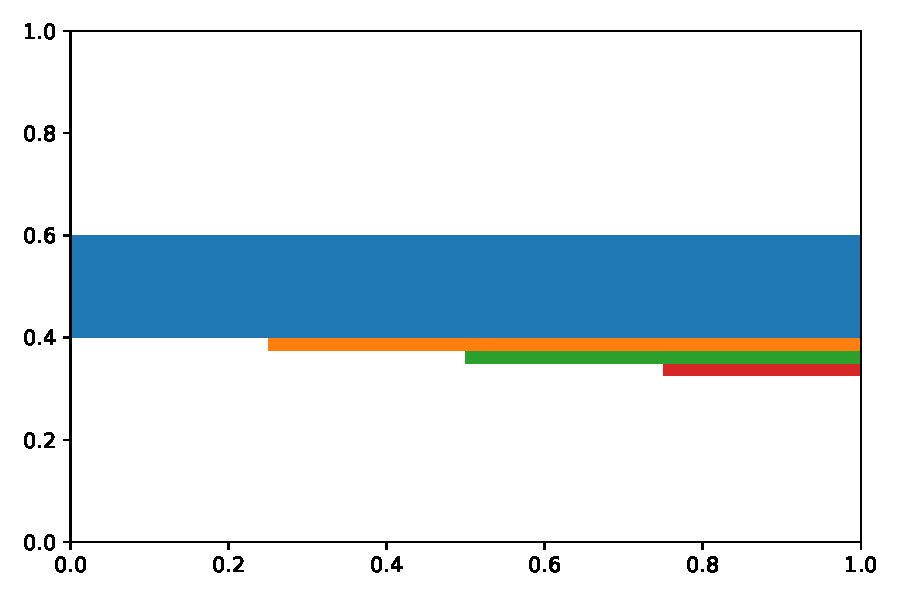
\includegraphics[width = .8\textwidth]{figures/proseplots/reverse-z.pdf}
\end{center}


\subsubsection{Axes and Tick Ordering}

Notice that by default, gridlines are ordered below artists added to a plot regardless of where the call to show the gridlines is placed. This can be changed using \code{ax.set_axisbelow()}, which also reorders the ticks. The \code{XAxis} and \text{YAxis} can be ordered independently using the \code{set_order()} axis method.

\pyfile{default-axes.py}

\begin{center}
    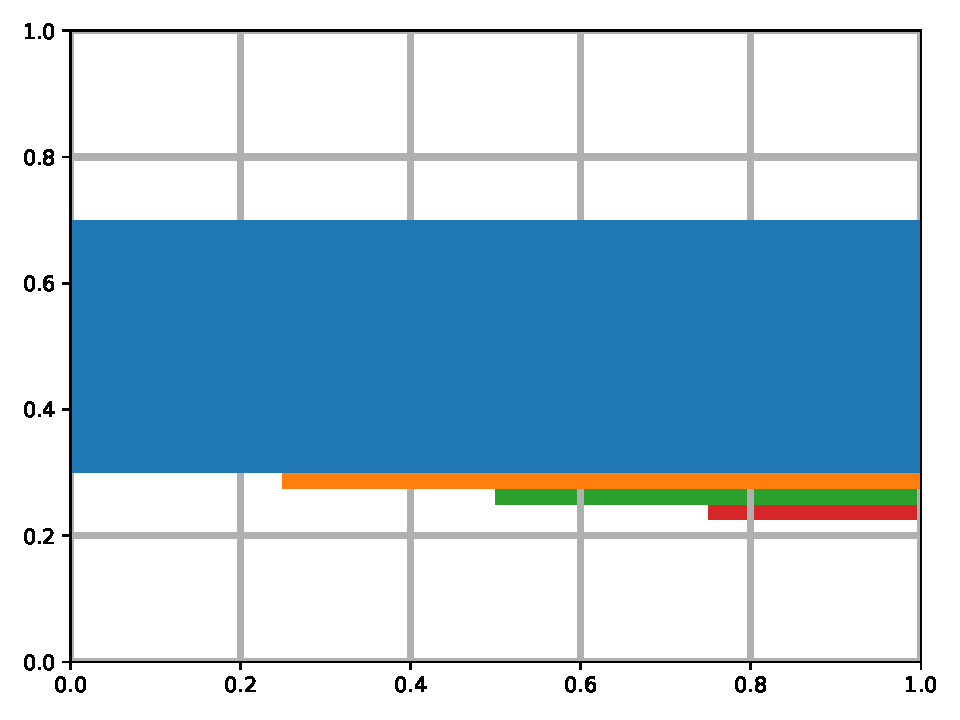
\includegraphics[width = .8\textwidth]{figures/proseplots/default-axes.pdf}
\end{center}

\pyfile{front-axes.py}

\begin{center}
    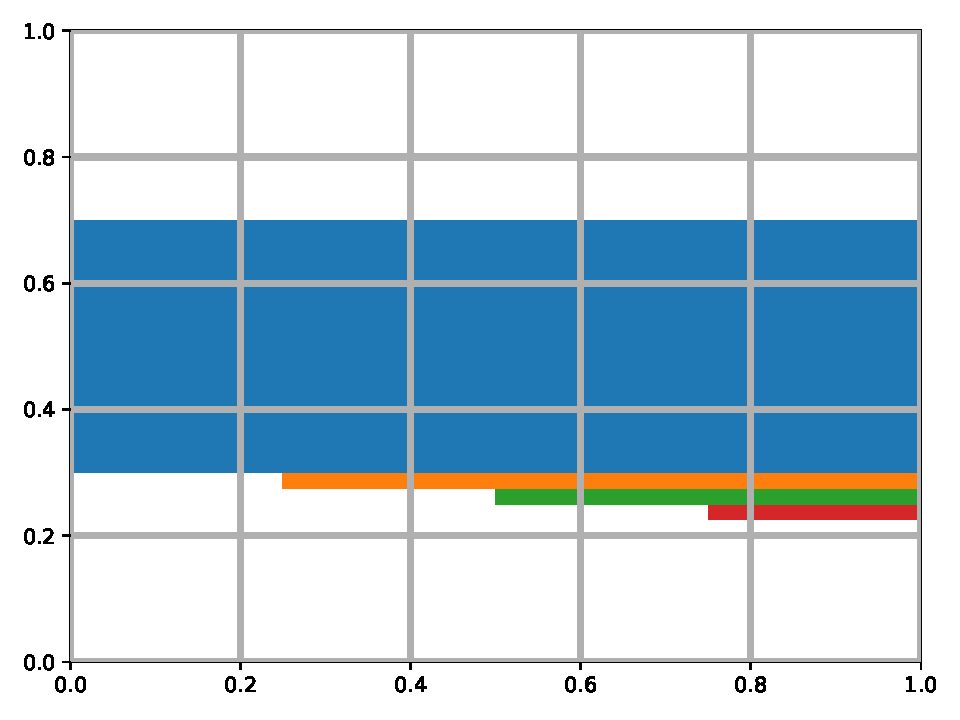
\includegraphics[width = .8\textwidth]{figures/proseplots/front-axes.pdf}
\end{center}

\pyfile{front-xaxis.py}

\begin{center}
    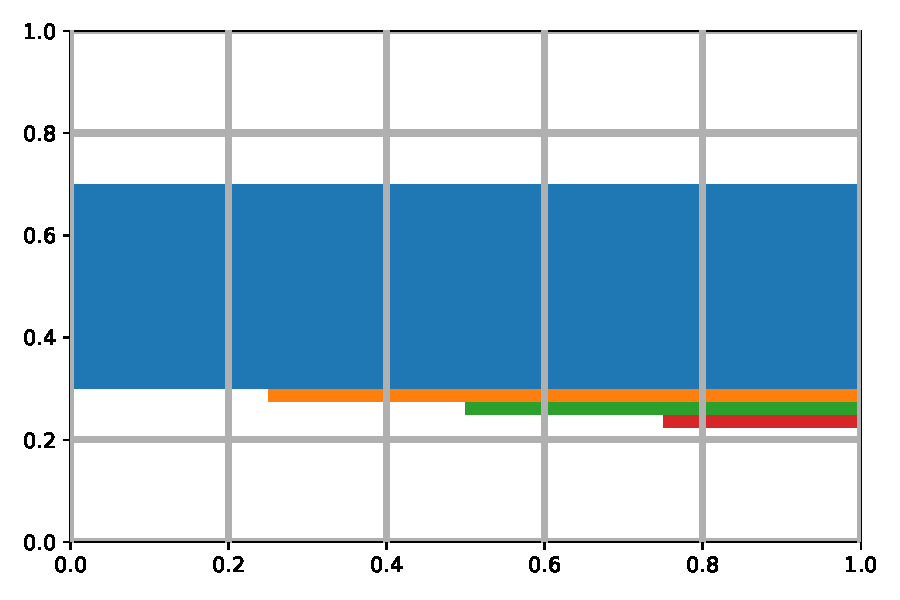
\includegraphics[width = .8\textwidth]{figures/proseplots/front-xaxis.pdf}
\end{center}


%https://matplotlib.org/stable/api/_as_gen/matplotlib.axes.Axes.set_axisbelow.html#matplotlib.axes.Axes.set_axisbelow
% https://matplotlib.org/stable/api/_as_gen/matplotlib.axes.Axes.fill_between.html


\section{Coordinate Systems and Transformations}

So far we have worked with data coordinates and you might not even realize there could be anything else. When we plotted a line between the points $(0,0)$ and $(1,1)$, we meant those as values in the usual $xy$-plane. But with use of transformations, we might also plot according to axes, figure, and display coordinates. In axes coordinates, $(0,0)$ is the bottom left of the axes and $(1,1)$ is the top right. Similarly, in figure coordinates, $(0,0)$ is the bottom left of the figure and $(1,1)$ is the top right. We won't cover the fourth type, display coordinates, which is the pixel coordinate system (for certain backends). The matplotlib \link{https://matplotlib.org/stable/tutorials/advanced/transforms_tutorial.html}{documentation} cautions that you should rarely work with display coordinates. However, display coordinates are a necessary evil when converting from one system to another. Note, it is important not to manipulate the figure or axes dimensions after referencing the display coordinate system or you might encounter unexpected behavior. 

The plot below features a group of plot calls using axes coordinates, then a group using figure coordinates, and then a single call using data coordinates. 
\pyfile{coords.py}

\begin{center}
    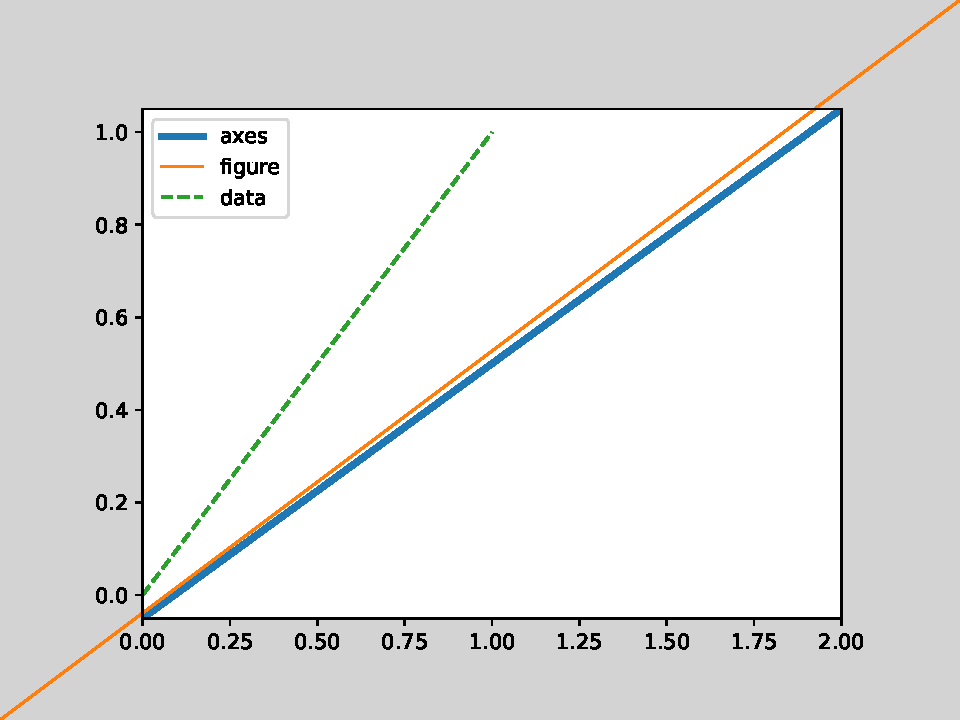
\includegraphics[width = .8\textwidth]{figures/proseplots/coords.pdf}
\end{center}


Axes and figure coordinates are often useful when you would like placement to be independent of the data, perhaps to enforce that something remain in the center of the plot by using an axes coordinate of 0.5. Below, we make use of that to set a vanishing point at the vertical halfway point.

\pyfile{coord-horizon.py}

\begin{center}
    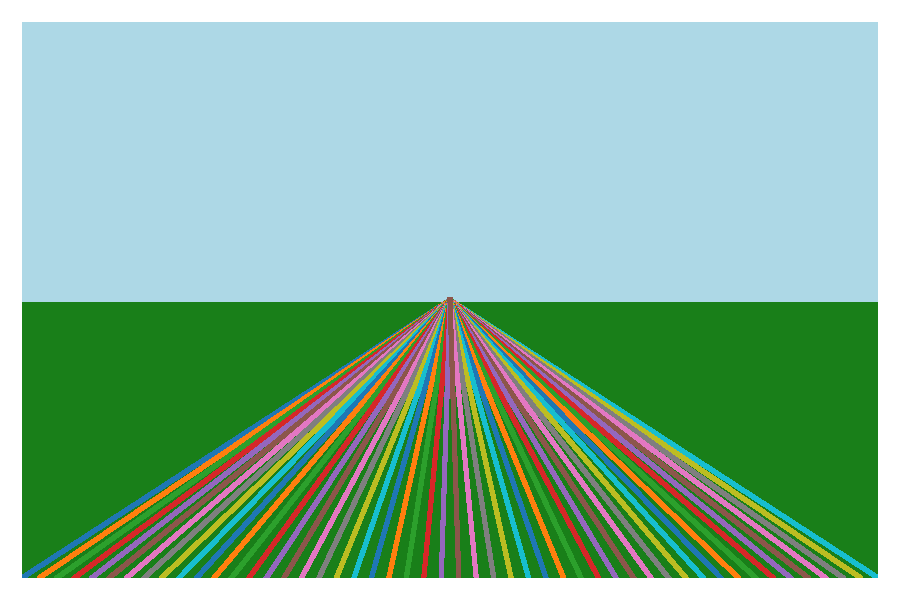
\includegraphics[width = .7\textwidth]{figures/proseplots/coord-horizon.pdf}
\end{center}


We can convert a point or sequence of points from one coordinate system to another using the appropriate transform object. \code{ax.transData.transform([x,y])} converts \code{x,y} from data coordinates to display coordinates. Simply replacing \code{ax.transData} with \code{ax.transAxes} or \code{fig.transFigure} converts from the corresponding coordinate system to display coordinates. The opposite direction is achieved by inverting the transformation---\code{ax.transData.inverted().transform([x,y])}. To go from data coordinates to figure or axes coordinates, you can make a pit stop in display coordinates. For example, \code{ax.transData.inverted().transform(ax.transAxes.transform([0.5, 0.5]))}  returns the middle of the axes window in data coordinates. The example below breaks this up into two steps. Again, take note that all plotting is done after setting a tight layout and after setting the axes limits to avoid resizing the figure and endangering the reliability of our coordinate transformations. 


\pyfile{coord-trans.py}

\begin{center}
    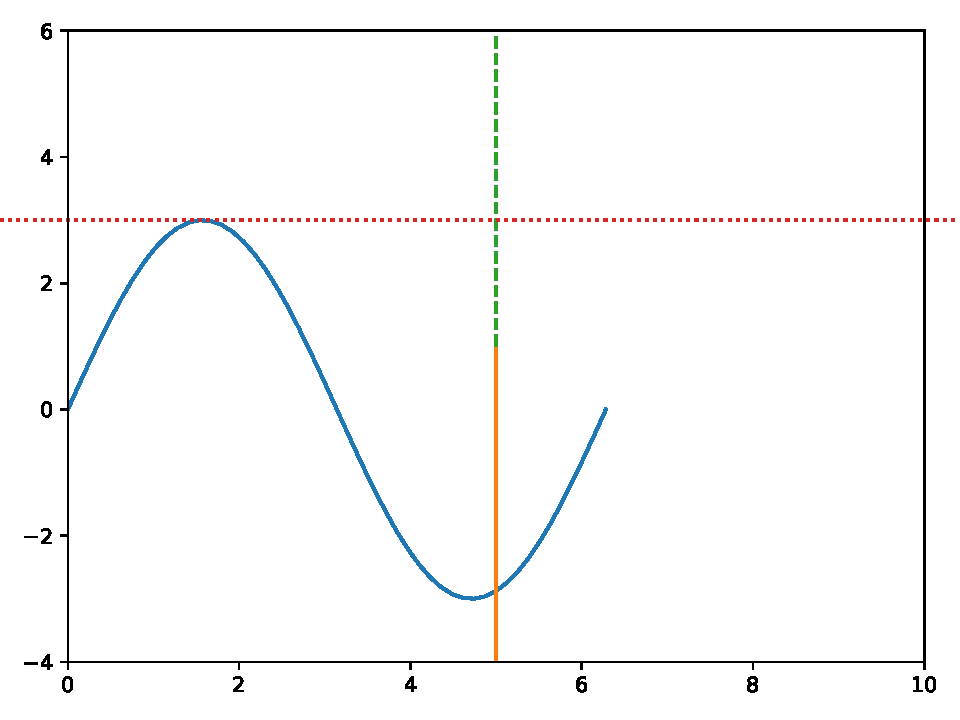
\includegraphics[width = .7\textwidth]{figures/proseplots/coord-trans.pdf}
\end{center}

%Let's test this by created a plot with a window extended 10 data units wide and 10 data units high. 


\section{Use Window Extents}

Another useful method is \code{get_window_extent()}, which allows you to find the bounding box (the coordinates for the corners of the enclosing rectangle) for something added to a plot. This can be used to find the display coordinates for where an annotation begins or ends, for example. Like in the previous section, note that the results will not update and be inaccurate if changes are made to the figure size, axes limits, or the canvas used. The method also requires a renderer. The technicalities for why can be put aside. Either include \code{fig.canvas.draw()} first, so the rendered is already cached, or include the argument \code{renderer = fig.canvas.get_renderer()} in the call to \code{get_window_extent()}. Below is a simple example. We create a text object with the axes method \code{ax.text()} in the normal way, but we take the atypical step of assigning the object to a variable. Below, that variable is named \code{center_text} and then we call \code{get_window_extent()} as a Text method, or an Artist method more abstractly. 

%Another atypical feature of \code{get_window_extent()} usage is the assigning the Text object to a variable \code{center_text} instead of simply running \code{ax.text()} to insert text. Below is straightforward example where we obtain the data coordinates for the bounding box of a Text object and then add vertical lines before and after the text.
%https://matplotlib.org/stable/api/_as_gen/matplotlib.artist.Artist.get_window_extent.html

\pyfile{window-extent.py}

\begin{center}
    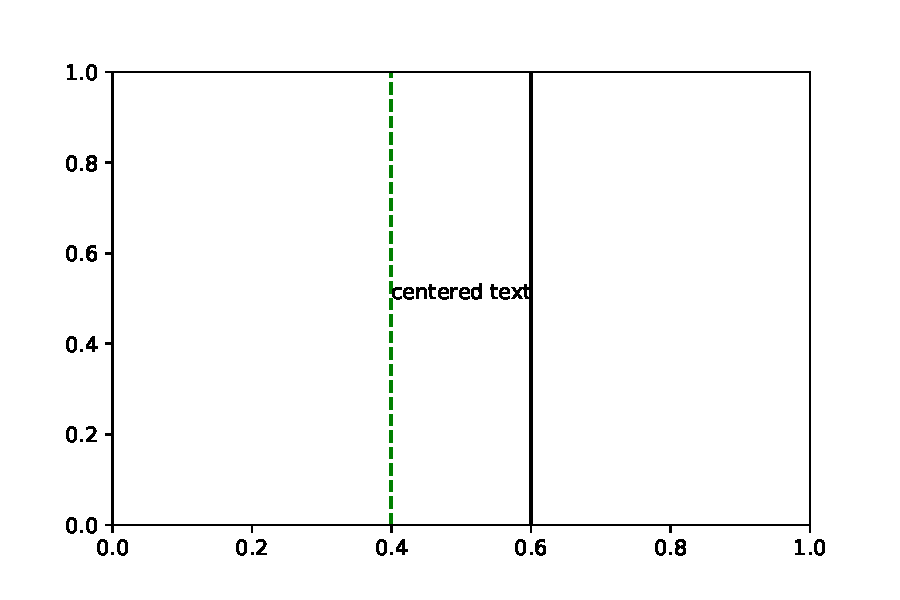
\includegraphics[width = .7\textwidth]{figures/proseplots/window-extent.pdf}
\end{center}

So what? A formatted title can stand in for a legend, helping reduce clutter. This helps us heed the call from \cite{schwabish2021better} to label data directly and avoid legends when possible. In the line chart below, a legend is unnecessary given the color-coding in the title. We create a title not with the typical \code{ax.set_title()} but with a series of \code{ax.text()} calls. There are several because a single Text object can't have multiple colors. The \code{ha} parameter is for horizontal alignment, and this is covered in more detail in a later chapter. By using \code{ha = 'left'}, the text will begin at the given $x$ and $y$ coordinates. % add reference when new chapter is added. 

\pyfile{multicolor-title.py}

\begin{center}
    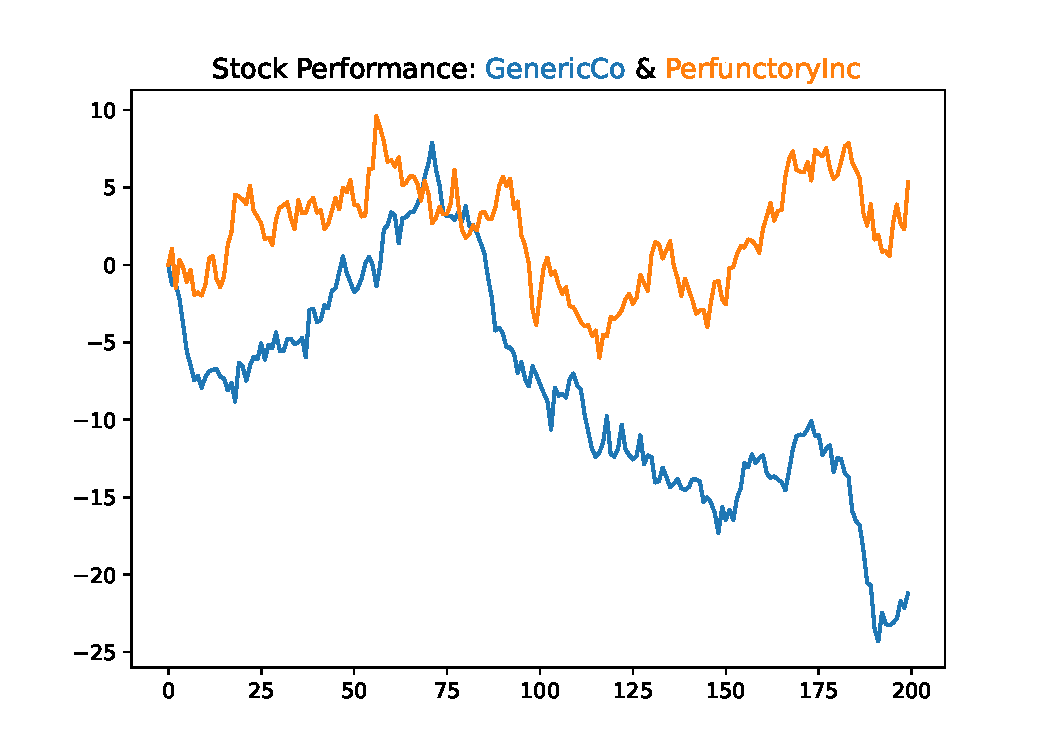
\includegraphics[width = .7\textwidth]{figures/proseplots/multicolor-title.pdf}
\end{center}




\chapter{Text and Titles}\label{chapter:titles}
\section{Simple Titles}

As we learned in Chapter \ref{chapter:oop}, we can add a title with the axes method \code{set_title()}. Simply pass the string of your choice as the argument. For multi-line titles, recall \code{\\n} can be used in a string to start a new line. Common optional arguments include \code{color}, \code{fontsize}, \code{weight}, and \code{loc}. 

Colors will be addressed in Chapter \ref{chapter:colors}, but to start you can simply use the name of any not-too-exotic color as a string.

\code{fontsize} (or \code{size}) can be a number or chosen from \code{'small'}, \code{'medium'}, or \code{'large'}, and \code{'small'} and \code{'large'} may be intensified with a \code{'x-'} or \code{'xx-'} prefix. Similarly, \code{weight} (or \code{fontweight}) can be a number or chosen from options like \code{'bold'} or \code{'light'}.

\code{loc} determines the location of the title, either \code{'left'}, \code{'center'}, or \code{'right'}. In the default style, the default value will be \code{'center'}. You might prefer using \code{'left'} to match the Google Sheets default (thus matching the vast majority of plots I've seen in industry). %Consider using \code{'left'} to match the Google Sheets default. 
\code{pad} controls the space between the title and the top of the axes. 


\pyfile{title-pad.py}

\begin{center}
    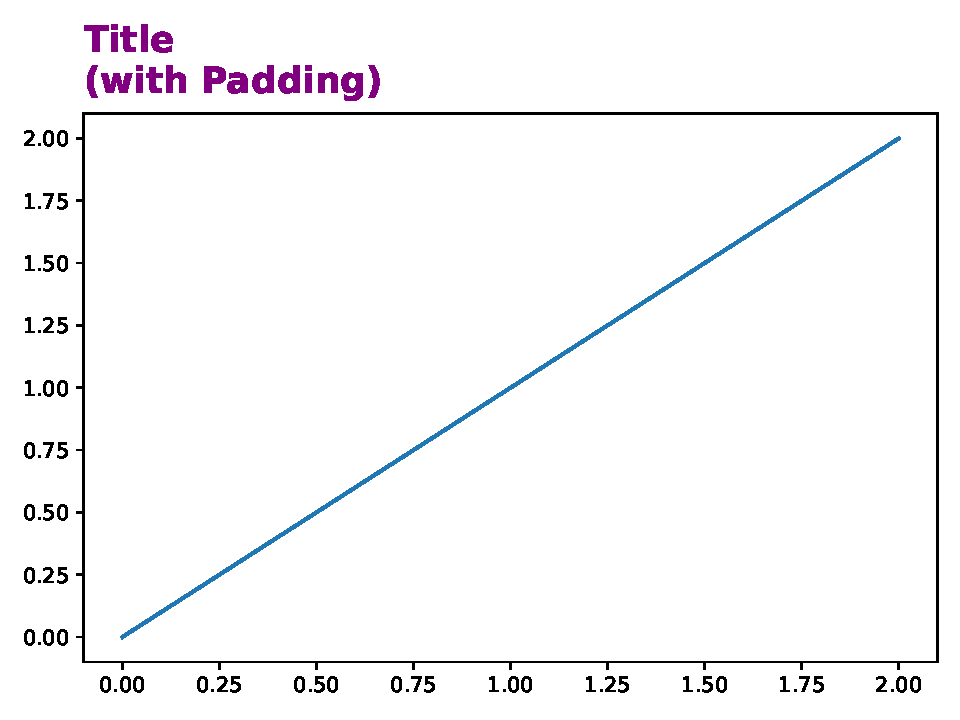
\includegraphics[width = .48\textwidth]{figures/proseplots/title-pad.pdf}
\end{center} \begin{center}
    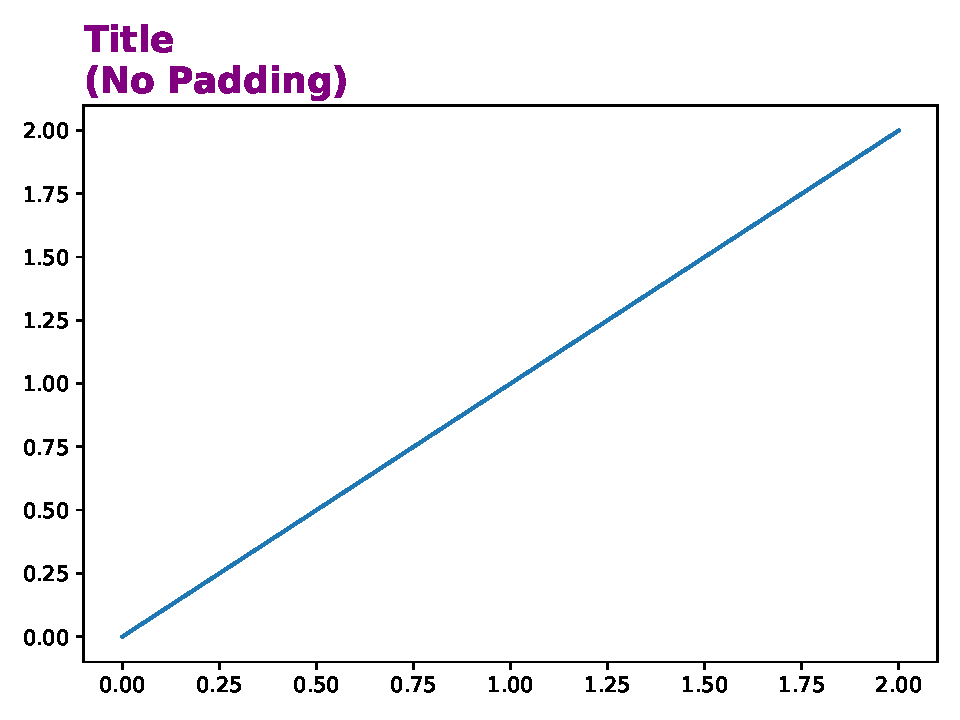
\includegraphics[width = .48\textwidth]{figures/proseplots/title-no-pad.pdf}
\end{center}

A plot can actually have one title for every \code{loc} value as well. 

\pyfile{title-loc.py}

\begin{center}
    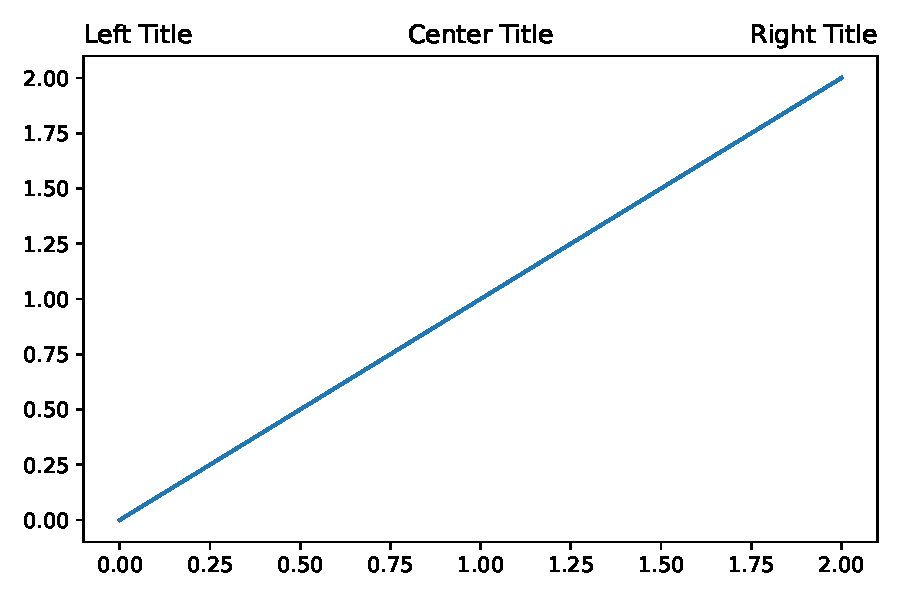
\includegraphics[width = .7\textwidth]{figures/proseplots/title-loc.pdf}
\end{center}


\section{Text and Placement}\label{sec:textplacement}

Matplotlib offers \code{text} as both a figure and an axes method. Let's start with some code to understand what they do. Both take $x$ and $y$ positions as the first two arguments and then a string. The figure method method is the same as using the axes method with a transformation to figure coordinates. 


\pyfile{text-methods.py}

\begin{center}
    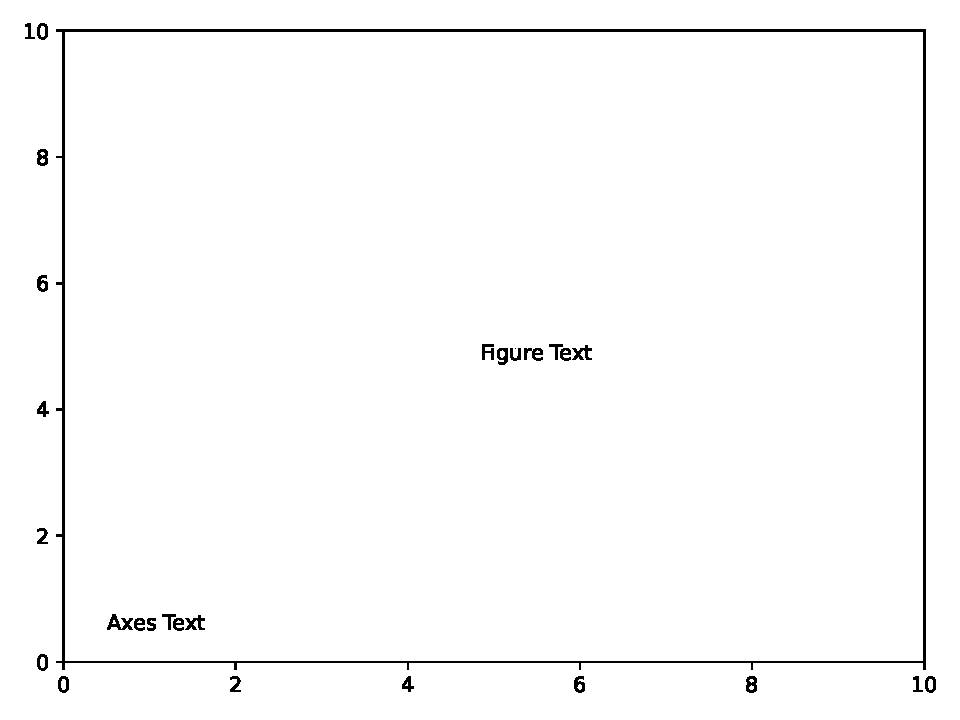
\includegraphics[width = .8\textwidth]{figures/proseplots/text-methods.pdf}
\end{center}

Immediately, we see that despite passing the same $x$ and $y$ position values, the figure and axes methods place the text differently. By default, the figure method uses ``figure'' coordinates, where (0,0) is the bottom left and (1,1) is the top right. The axes method uses $x$ and $y$ data coordinates by default. We will modify this shortly. 

A more common concern is the alignment of the text. Both figure and axes text methods include parameters \code{verticalalignment} and \code{horizontalalignment}, which can be abbreviated as \code{va} and \code{ha}. By default, the text is placed so that the given coordinate is at the bottom-left corner of the text. 

\pyfile{text-default-align.py}

\begin{center}
    
\includegraphics[width = 0.5\textwidth]{figures/proseplots/text-default-align.pdf}
\end{center}

\noindent For vertical alignment, the options are \code{'top'}, \code{'bottom'}, or \code{'center'}. For horizontal alignment, the options are \code{'left'}, \code{'right'}, or \code{'center'}. The default demonstrated above was \code{'bottom'} and \code{'left'}. It does result in the text being above and to the right of the coordinate point, perhaps confusingly, but the interpretation is that the coordinate point is at the bottom-left of the text. The possible alignments are illustrated below. 

\pyfile{text-align.py}

\begin{center}
    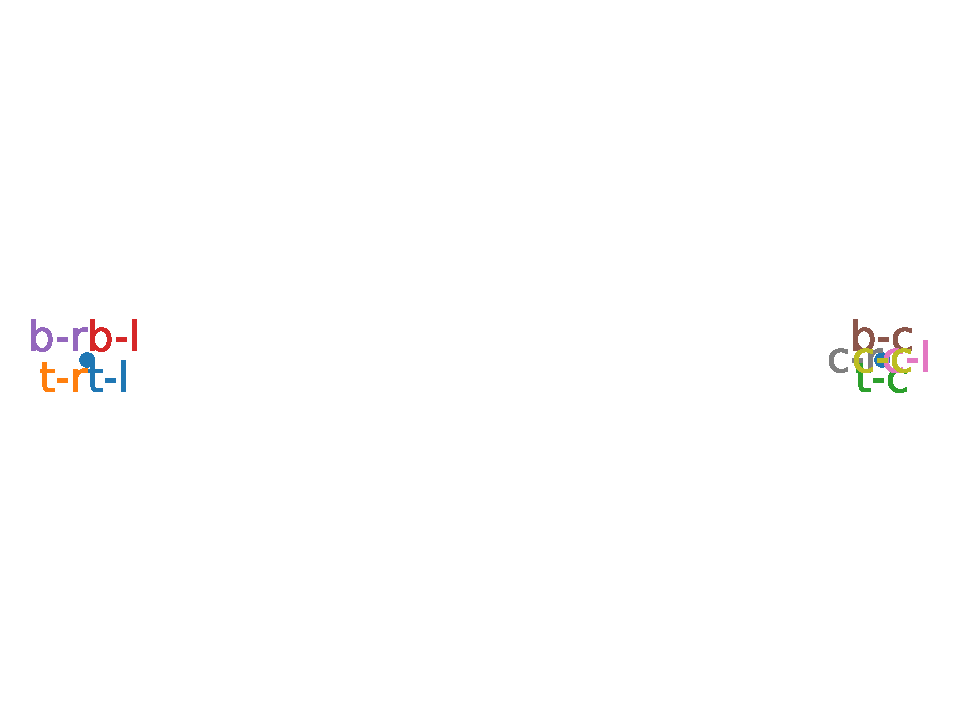
\includegraphics[width = 0.7\textwidth]{figures/proseplots/text-align.pdf}
\end{center}


Text can be rotated with the \code{rotation} parameter. By default, a plot isn't square---the aspect ratio (the ratio of $y$-unit to $x$-unit) is not one. That means that the 45 degree line created by $y=x$ is not actually plotted at 45 degrees. Yet according to the \code{rotation} parameter, text rotated at 45 degrees is plotted at 45 degrees---that angle is not converted based on the aspect ratio. Later in Section \ref{sec:slopingtext}, I go into further detail in how to use some trigonometry to get the exact angle if you'd like to slope text at some angle, accounting for the aspect ratio. 

\pyfile{text-rotation2.py}


\begin{center}
    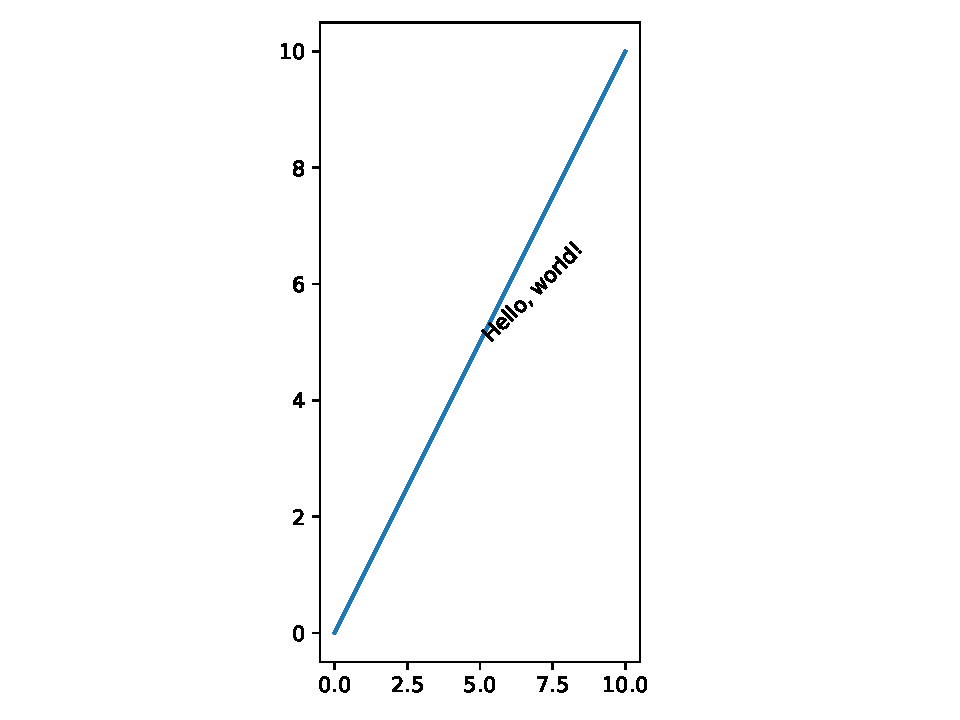
\includegraphics[width = 0.33\textwidth]{figures/proseplots/text-rotation2.pdf}
\end{center} \begin{center}
    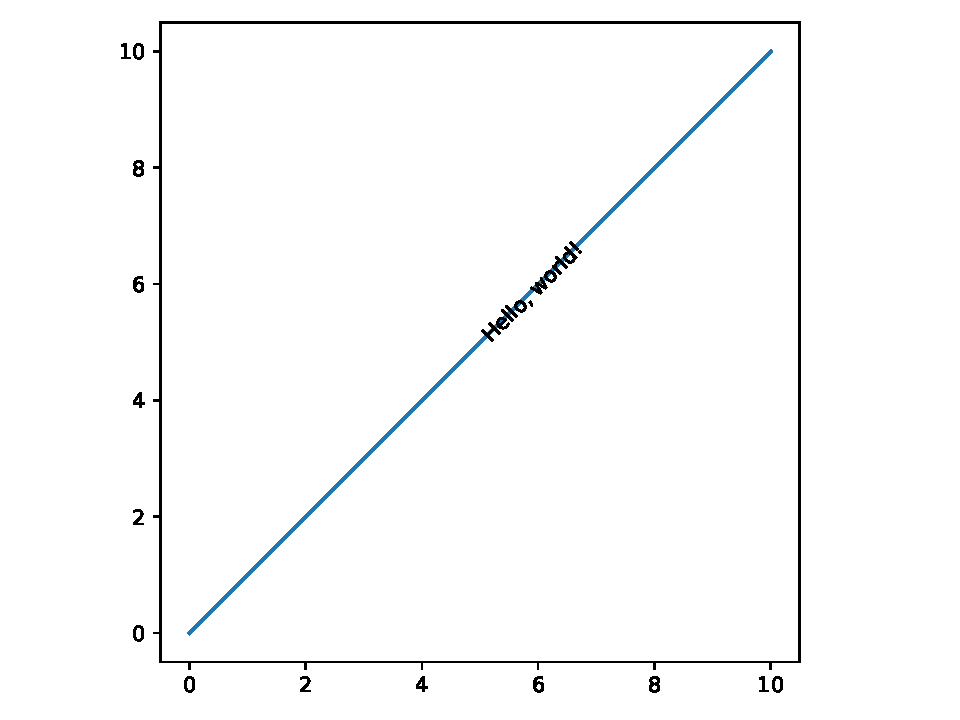
\includegraphics[width = 0.33\textwidth]{figures/proseplots/text-rotation1.pdf}
\end{center} \begin{center}
    \includegraphics[width = 0.33\textwidth]{figures/proseplots/text-rotation05.pdf}
\end{center}


%\vspace{-1cm}

%https://matplotlib.org/stable/tutorials/advanced/transforms_tutorial.html

%\subsection{Coordinate System Transformations}
%Now we return to the fact that \code{ax.text()} uses data coordinates by default, among all the possible coordinate systems described in Chapter \ref{chapter:elements}. This can be changed using the \code{transform} parameter, selecting from a number of possible transformations. Using \code{transform = ax.transAxes}, the $x$ and $y$ positions are based on the coordinate system of the axes object, where (0,0) is the bottom left and (1,1) is the top right. This is different than the default behavior of \code{fig.text()} which is based on the larger figure object. Below, observe that the figure text, in blue, is centered with respect to the larger figure (the axes and the light yellow background). The axes text is centered with respect to the axes which sits slightly right of center in the larger figure. 

%\begin{lstlisting}[language = Python]
%fig, ax = plt.figure(facecolor = 'lightyellow'), plt.axes()
%ax.set_xlim([0,10])
%ax.set_ylim([0,10])
%fig.text(0.5, 0.5, 'Z', 
%    ha = 'center', va = 'center', 
%    color = 'C0', fontsize = 50)
%ax.text(0.5, 0.5, 'Z', 
%    transform = ax.transAxes, 
%    ha = 'center', va = 'center',
%    color = 'C1', fontsize = 50)
%\end{lstlisting}


%\begin{center}
  %  \includegraphics[width = .8\textwidth]{proseplots/texttransform1.pdf}
%\end{center}

%You might also find it useful to blend two transformations, allowing you to, for example, mix data coordinates in one dimension with axes coordinates in another. 
%You can learn more about the other available transformations from the \link{https://matplotlib.org/stable/tutorials/advanced/transforms\_tutorial.html}{matplotlib tutorial}\footnote{https://matplotlib.org/stable/tutorials/advanced/transforms\_tutorial.html}.
%By default, a plot usually isn't square---the aspect ratio (the ratio of $y$-unit to $x$-unit) is not one. That means that the 45 degree line created by $y=x$ is not actually plotted at 45 degrees. Yet according to the \code{rotation} argument, text rotated at 45 degrees is plotted at 45 degrees---that angle is not converted based on the aspect ratio. Later in Section \ref{sec:slopingtext}, I go into further detail in how to use some trigonometry to get the exact angle if you'd like to slope text at some angle, accounting for the aspect ratio. 

\subsection{Text Formatting for Numbers}\label{subsec:textformat}
Here I've tucked away a subsection on formatting numbers in Python. This has nothing to do with matplotlib, formally speaking. Still, sometimes you want your text annotations or titles to contain numbers formatted just so and you'll want Python to figure that out instead of doing it by hand. You might want commas as the thousands separator (the more readable 1,000,000 instead of 1000000), you might want leading zeros (01 instead of 1), or you might want a currency symbol (\$2 instead of 2). The table below demonstrates by example how to do this with \code{str.format}.

\begin{center}
{\setlength{\tabcolsep}{2em}
\begin{tabular}{ll}
\toprule
Code & Output \\
\midrule
\code{'\{:,\}'.format(10**6)} &    \code{'1,000,000'} \\
\code{'\$\{:,.2f\}'.format(10**6)} & \code{'\$1,000,000.00'} \\
\code{'\{:0>3.0f\}'.format(1)}  &    \code{'001'}\\
\code{'\{:>3.0f\}'.format(1)}  &    \code{'  1'} \\
\code{'\$\{:0>4.0f\}'.format(1)}  &   \code{'\$0001'} \\
\code{'\{:+,.1f\}'.format(1000)} & \code{'+1,000.0'} \\
\code{'\{:0<+4,.1f\}'.format(-1)} & \code{'-1.0'} \\
\code{'\{:0<5.0f\}'.format(1)}  &    \code{'10000'} \\
\code{'\{:0<5,.0f\}'.format(1)}  &    \code{'10000'} \\
\code{'\{:0<8,.0f\}'.format(1000)} &  \code{'1,000000'} \\ 
\code{'\{:.0e\}'.format(10.1**6)} & \code{'1e+06'} \\
\code{'\{:.1f\} and \{:.1f\}'.format(9, 1)} & \code{'9.0 and 1.0'} \\
\code{'\{1:.1f\} and \{0:.1f\}'.format(9, 1)} & \code{'1.0 and 9.0'} \\
\code{'\{0:\} and \{0\}'.format(1)} & \code{'1 and 1'} \\
\code{'\{:\} and \{:\}'.format(1)} & \code{IndexError}\\
\bottomrule
\end{tabular}}
\end{center}

Understanding everything above requires some knowledge of \link{https://docs.python.org/3/library/string.html\#format-specification-mini-language}{format specifications}. A format specifier is a string that can specify fill, align, sign, width, grouping option, precision, and type (\lstinline{[[fill]align][sign][#][0][width][grouping_option][.precision][type]}. These must be properly ordered but anything can be omitted to accept the default. These arguments go inside curly braces and to the right of a colon, \code{\{:\}}. The curly braces tell Python where to place the argument you pass to the \code{format()} method. You can also pass multiple arguments inside \code{format()}. By default, they are placed in order (the first argument replaces the first \code{\{\}} and so on), but to the left of the colon, you can also specify the index value for the argument to use.

The \emph{fill} is a character that can be used to pad the number. Used with a \emph{align} and \emph{width}, we can add leading zeros. The default is a space if no fill character is provided. Using \code{'0>4'}, this will create leading zeros (right-aligned) up to a width of 4. So \code{1} becomes \code{'0001'} and \code{10000} is not padded, being simply \code{'10000'}. 

The \emph{grouping option} would come next, allowing for a thousands separator of a comma or an underscore. \code{'\{:,\}'.format(10000)} produces \code{'10,000'}. Note that when used with padded numerals on the right, the padding is ignored in finding the thousands separators, so \code{'\{:0<8,.0f\}'.format(1000)} produces the confusing \code{'1,000000'}.

\emph{Precision} is next with a decimal and then how many digits to display past the decimal place or before and after, depending on the lastly specified \emph{type}. Observe \code{'\{:.2\}'.format(np.pi)} produces \code{'3.1'} and \code{'\{:.2f\}'.format(np.pi)} produces \code{'3.14'}. You'll want type \code{'f'} for a float. Use \code{'e'} for scientific notation. You may read up on the many other types, including locale aware types, in the Python documentation.\footnote{https://docs.python.org/3/library/string.html\#grammar-token-type}

Whatever we put outside the curly braces is simply concatenated to the text on the left or right. So \code{'\$\{\}'.format(123)} turns 123 into the dollar figure \code{'\$1231'}. And \code{'\{\} lbs.'.format(123)} would produce \code{'1231 lbs'}. 

Perhaps this will come in handy when you'd like figure text or the filename in a certain format. I often use leading zeros in some filenames so that alphabetically ordering the files will be coherent (your file system will likely maintain \code{'1' < '10' < '2'}). If you are creating many plots that will be frames in an animation, and you'll have some number ticking up as the frames progress, the padding might help the eye.  

\pyfile{text-formatting.py}

\begin{center}
    \includegraphics[width = 0.3\textwidth]{figures/proseplots/0000.pdf} \includegraphics[width = 0.3\textwidth]{figures/proseplots/0001.pdf}
     \includegraphics[width = 0.3\textwidth]{figures/proseplots/0002.pdf}
\end{center}

\section{Legends}
As you should know, legends provide a key to the colors and symbols used in a plot. You can create a legend with \code{legend()}, as either a figure or axes method. Without any extra customization this is done with \code{ax.legend()} or \code{fig.legend()}. Here, we will only cover axes legends. We'll return to figure legends when they are more naturally useful in Chapter \ref{chapter:multi} on multiple axes and multiple plots. 

But first, you need labels for your plot elements (called \emph{artist} objects) before you can create a legend. This can be done with the \code{label} parameter in methods like \code{plot()}. Or you can use \code{set_label()} on the plot element object. Using \code{set_label()} adds some complication to the code, as seen below in an otherwise simple example. Note the legend needs to be added after the labeled plot elements you want included in the legend.


\pyfile{legend-labels.py}

\begin{center}
    \includegraphics[width = .7\textwidth]{figures/proseplots/legend-labels.pdf}
\end{center}

If you are using a pandas plot method, the labels will be set automatically according to the column or series names. For such instances where an element is automatically included in a legend and you want to exclude it, you can exclude that element by specifying \code{label = '_nolegend_'} in the plot call.


\pyfile{pd-legend.py}


\begin{center}
    \includegraphics[width = .7\textwidth]{figures/proseplots/pd-legend.pdf}
\end{center}


A more common concern might be how to customize the placement of the legend and its actual appearance. 

To change the placement of the legend, you may use the \code{loc} parameter. The default value is \code{'best'}, where best is determined by matplotlib. Other valid values are \code{'center'} and \code{'right'} (but not \code{'left'}) and then modifications like \code{'upper center'}, \code{'center right'}, and \code{'lower left'}. 

For further customization of the placement, use the \code{bbox_to_anchor} parameter. This accepts 2-tuple or 4-tuple, giving the $x$ location, the $y$ location, and the width and height optionally.

By default, $x$ and $y$ are in axes coordinates. So the program below places a legend in the top and center of the axes. The alignment is done accodring to \code{loc}. If, for example, \code{loc = 'lower right'}, then the lower right corner of the legend is placed at the specified $x$ and $y$. 

\pyfile{legend-bb.py}

\begin{center}
    \includegraphics[width = .7\textwidth]{figures/proseplots/legend-bb.pdf}
\end{center}

\pyfile{legend-bb-loc.py}

\begin{center}
    \includegraphics[width = .7\textwidth]{figures/proseplots/legend-bb-loc.pdf}
\end{center}
If using a 4-tuple, the tuple is interpreted as the plot region in which to put the legend, according to \code{loc}. 

Use \code{bbox_transform} to use a coordinate system other than the default axes coordinates. 

\pyfile{legend-transform.py}

\begin{center}
    \includegraphics[width = .7\textwidth]{figures/proseplots/legend-transform.pdf}
\end{center}

There are many parameters to change the appearance of the legend. We won't cover all of them. Two useful parameters are \code{facecolor} and \code{ncol}. The former changes the background color of the legend and the latter sets the number of columns, changing the default shape of the legend. I use these and a few other self-explanatory parameters in the program below. 

\pyfile{legend-shape.py}

\begin{center}
    \includegraphics[width = .7\textwidth]{figures/proseplots/legend-shape.pdf}
\end{center}


\section{Annotations}

\cite{knaflic2015storytelling} and \cite{schwabish2021better} both advise to label data directly and to annotate graphs with explanatory notes when helpful, as this helps convey the meaning of the graph more simply and directly. 

You can annotate a chart with \code{text()} method calls, or you can use the \code{annotate()} method, for which you specify the text placement and a line segment to the part of the graph the text references. 


\subsection{Labeling and Arrows}

The following graph is nothing special, but we avoid having to create a legend by labeling the data with the text color matching the line color. 

\pyfile{label-data.py}

\begin{center}
    \includegraphics[width = .7\textwidth]{figures/proseplots/label-data.pdf}
\end{center}


Next, we use the \code{annotate()} method. This method comes with the option to include an arrow pointing from \code{xytext} to the point \code{xy}. 

\pyfile{annotate-arrow.py}

\begin{center}
    \includegraphics[width = .7\textwidth]{figures/proseplots/annotate-arrow.pdf}
\end{center}


If you would like an arrow and no text, simply use the empty string \code{''}. It is necessary to pass a dictionary to the \code{arrowprops} property. 

\pyfile{arrow-only.py}

\begin{center}
    \includegraphics[width = .7\textwidth]{figures/proseplots/arrow-only.pdf}
\end{center}


Lastly, one can also reference specific artist objects in the annotation instead of coordinates. In the below we place the annotations at the end of \code{a_line} and \code{b_line}.  

\pyfile{direct-annotation.py}

\begin{center}
    \includegraphics[width = .7\textwidth]{figures/proseplots/direct-annotation.pdf}
\end{center}


%Now we are going to label our graph not by using the data itself, but by referencing the lines and patches. 

\section{Fancy Titles}
If you'd like to format different parts of the title different, you'll have to move beyond simply using \code{set_title}. The New York Times, for example, routinely includes a title and a subtitle in a plot. This requires using \code{text()} and \code{set_title()} separately, as there can only be one format style applied to a title. A simple example is below.

\pyfile{subtitle.py}

\begin{center}
    \includegraphics[width = .80\textwidth]{figures/proseplots/subtitle.pdf}
\end{center}


\subsection{Multi-colored Titles}


In Chapter \ref{chapter:elements}, we created a multi-colored title using the Artist method \code{get_window_extent()}. The advantage of a multi-colored title is that we can do without a legend. For someone who doesn't want to get into the complications of \code{get_window_extent()}, the $x$ and $y$ placement of the text could be done by sight. 

\pyfile{multicolor-inexact.py}

\begin{center}
    \includegraphics[width = .80\textwidth]{figures/proseplots/multicolor-inexact.pdf}
\end{center}

Greater elegance requires greater complication. If you are (understandably) dissatisfied with the above, invest in the topics covered in Chapter \ref{chapter:elements}. 
Below, we build on the solution from Chapter \code{chapter:elements} by creating a function that creates a multi-colored title. Note we remove text options with the \code{remove()} method and work all in a single figure. This replaces the work of tuning the centering by hand that was done previously. 

\pyfile{color-title.py}

\pyfile{color-title-ex.py}

\begin{center}
    \includegraphics[width = .80\textwidth]{figures/proseplots/color-title-ex.pdf}
\end{center}

\section{Fonts}

Finally, you might want to customize the fonts. First, we'll consider the customizations available in matplotlib by default. 

% t.get_font().__dict__


\subsection{Importing Fonts with Font Manager}
If you're unsatisfied with the basic fonts available in matplotlib, just add your own. You can find fonts available for download from \link{https://www.theleagueofmoveabletype.com/}{theleagueofmoveabletype.com} or \link{https://fonts.google.com}{fonts.google.com}. 

After you've downloaded a font family, you should have folder for that font with otf or ttf files. Matplotlib has a font manager and you just need to tell matplotlib to look for a font in that folder. This is done below using \code{fintSystemFonts()} and \code{addfont()}. Once the font files are added, you can simply specify the font in the \code{text()} call like any other in-built font. 

\pyfile{font.py}


\begin{center}
    \includegraphics[width = .7\textwidth]{figures/proseplots/font.pdf}
\end{center}


\chapter{Dates}\label{chapter:dates}
Matplotlib can handle dates, helping you to create better axis ticks and label formatting. Matplotlibs capabilities are built on the datetime and dateutil modules. 


\section{Plotting}
Let's import some time series data. Below we use pandas integration and plot from a DataFrame with an index of pandas Timestamp values. Matplotlib recognizes these as dates and handles this reasonably well automatically, though the exact formatting could be improved. 

\pyfile{pd-dates.py}

\begin{center}
    \includegraphics[width = .7\textwidth]{figures/proseplots/pd-dates.pdf}
\end{center}

Before we try to improve the formatting, see what happens if we try to use the axes plot method. 

\pyfile{ax-dates.py}

\begin{center}
    \includegraphics[width = .7\textwidth]{figures/proseplots/ax-dates.pdf}
\end{center}

In the old days, \code{plot_date()} was used in place of \code{plot()}, but this is no longer necessary.


\subsection{Time Zone Handling}

%\code{plot_date()} also plots the dates according to a default UTC timezone, sometimes converting dates given in a different timezone. This can be modified with the \code{tz} parameter, but this requires covering 


For a deeper knowledge, see the \code{datetime.tzinfo} class and the \code{pytz} library. 

\section{Ticks and Formatting}


\subsection{Date Formats}

The specific format of the displayed dates and times can be modified with \code{mdates.DateFormatter()}. This takes a format string and creates a formatter that can be passed to an axis method \code{set_major_formatter()} or \code{set_minor_formatter()}. 

Here are some common format codes, applied to Sunday January 30, 2000, 11:59PM, local to Louisville, Kentucky. These can all be verified with \code{pd.Timestamp(year = 2000, month = 1, day = 30, hour = 23, minute = 59, tz = 'America/Kentucky/Louisville').strftime()}.

\begin{center}
\begin{small}
{\setlength{\tabcolsep}{2em}
\begin{tabular}{ll}
\toprule
Code & Output/Example \\
\midrule
\code{'\%Y'} & 4-Digit Year \\
\code{'\%m'} & Month Number \\
\code{'\%d'} & Day of Month \\
\code{'\%B'} & Month Name \\
\code{'\%H'} & 24-Hour Clock Hour \\
\code{'\%M'} & Minute \\
\code{'\%H'} & 12-Hour Clock Hour \\
\code{'\%p'} & AM or PM \\
\code{'\%A'} & Day of Week \\
\code{'\%Z'} & Timezone Name \\
\code{'\%Y-\%m'} &   \code{'2000-01'}\\
\code{'\%Y\/\%m/\%d'} & \code{'2000/01/30'}\\
\code{'\%B \%y'} & \code{'January 00'}\\
\code{'\%H:\%M \%Z'} & \code{'23:59 EST'} \\
\code{'\%A \%I\%p'} & \code{'Sunday 11PM'}\\
\bottomrule
\end{tabular}}
\end{small}
\end{center}

A more complete list of format codes can be found at \link{https://strftime.org}{strftime.org}. Codes that generate actual names, like \code{'\%A'} or \code{'\%B'}, can be made lowercase to produce an abbreviated name. Notice that these formats create zero-padded numbers like \code{'07'} instead of \code{'7'}. On Mac or Linux, padding can be eliminated with the \code{'-'} modifier, using \code{'\%-H'} or \code{'\%-m'}
instead of \code{'\%H'} or \code{'\%m'} for example. On Windows, use \code{'#'}.

\pyfile{date-fmt.py}

\begin{center}
    \includegraphics[width = .7\textwidth]{figures/proseplots/date-fmt.pdf}
\end{center}

\pyfile{date-fmt2.py}

\begin{center}
    \includegraphics[width = .7\textwidth]{figures/proseplots/date-fmt2.pdf}
\end{center}


\chapter{Colors}\label{chapter:colors}
Methods like \code{plot} and \code{text} include a color parameter, which we've already made use of. While you can get pretty far simply using \code{color = 'blue'}, you might also make use of colormaps or set your own colors using hex strings or RGB(A) tuples. 

\section{Colormaps}

According to the style sheet you are using, there will be some colormap and you will cycle through those colors by default when plotting (but not for text). The colors can be identified by the strings \code{'C0'}, \code{'C1'}, \dots. If, as in the default, your color map has only 10 distinct colors, then the eleventh color \code{'C10'} is valid, but simply refers to \code{'C0'} and the colors cycle from there. You'll notice that with successive plot calls on the same axes, the colors will automatically move through the colormap. This is not the case with text, as is demonstrated in the program below. 

\pyfile{colors.py}

 \begin{center}
     \includegraphics[width = 0.7\textwidth]{figures/proseplots/colors.pdf}
 \end{center}
 
 
 \section{Red, Green, Blue, Alpha}
 
 An RGB color is given by three values, specifying the amount of red, green, and blue. In matplotlib, these values are between zero and one (you might also see RGB values between zero and 255 elsewhere). These colors live inside a cube, as a particular color is a triple $(r,g,b) \in [0,1]^3$. 

\begin{center}
    \includegraphics[width = .49\textwidth]{figures/proseplots/color-cube.pdf}\includegraphics[width = .49\textwidth]{figures/proseplots/color-cube-back.pdf}
\end{center}
% https://stackoverflow.com/questions/8130823/set-matplotlib-3d-plot-aspect-ratio/19933125

I like working with RGB tuples because they can be manipulated with mathematical operations. Two colors can easily be averaged or we can create a gradient between two. 

\pyfile{gradient.py}

\begin{center}
    \includegraphics[width=.8\textwidth]{figures/proseplots/gradient.pdf}
\end{center}

Any color can be made lighter by averaging it with white, $(1,1,1)$, or darker by averaging it with black $(0,0,0)$. We can also find the inverse of an RGB color by simply subtracting that triple from  $(1,1,1)$. RGBA tuples are very similar, adding a fourth \emph{a}lpha value for the opacity. 


With RGB and RGBA colors being so handy, you might want to convert strings like \code{'C0'} into RGB. \code{ColorConverter()} lets us do this, with the \code{to_rgb()} and \code{to_rgba()} methods. Below, we create another color gradient between the default \code{'C0'} blue, to \code{'C1'} orange, and on to light blue \code{'C9'}.

\pyfile{color-map.py}

\begin{center}
    \includegraphics[width = .8\textwidth]{figures/proseplots/color-map.pdf}
\end{center}



\subsection*{Color Cube Code}
Here is the code for one of the RGB color cubes.  

\pyfile{color-cube.py}

\chapter{Multiple Axes and Plots}\label{chapter:multi}
\section{Multiple Axes}
% add two histograms as a bad example
% https://stackoverflow.com/questions/6871201/plot-two-histograms-on-single-chart-with-matplotlib

Let's start with a concrete goal to help illustrate possible uses of multiple axes. We want to plot a standard normal distribution. This is the familiar bell curve with a range of possible draws from the normal distribution on the $x$-axis and $y$ values are the value of the probability density function (PDF) evaluated at each $x$ value. Furthermore, we have a $z$-score and we want the visual to help us see how often we should get smaller $z$-scores if we are sampling from this distribution. In particular, let's say our $z$-score is 0.674. 

To answer the question narrowly, the following plot does the job well and without reaching for multiple $x$- or $y$-axes. 

\pyfile{norm-pdf.py}

\begin{center}
\includegraphics[width = .7\textwidth]{figures/proseplots/norm-pdf.pdf}
\end{center}

Still, it leaves the reader to rely on their eyeballing abilities to imagine how that area might change if the $z$-score changed. The graph itself lacks information from the cumulative density function (CDF), used to calculate that our $z$-score at the 75\%ile of values drawn from the standard normal distribution. If your reader might be interested in this kind of thought exercise, you should include more of this information in the plot. First, we might add this information by simply plotting both the PDF and CDF together. Eyeballing is still necessary to imagine how much rarer a $z$-score of 0.7 is, but at least with the CDF included, we can be a little more precise. 

\pyfile{cdf-pdf.py}

\begin{center}
    \includegraphics[width = .7\textwidth]{figures/proseplots/cdf-pdf.pdf}
\end{center}

Still, the plot above isn't very good. Here, more ticks or a grid would be helpful for tracing out what the CDF value is for a particular $z$-score. But apart from that, you might also see that the orange CDF dwarfs the blue PDF. While not terribly extreme, these functions cover different enough $y$ values that having a shared $y$-axis is questionable, because the point isn't to draw attention to this difference. One fix for this is to create a second $y$-axis on the right. \cite{knaflic2015storytelling} advises against a secondary $y$-axis. Dual axis charts aren't as immediately readable, so do be judicious and take extra care to make it clear which plot corresponds to which $y$-axis.

\subsection{Using \code{twinx()} and \code{twiny()}}

If we want a second $y$-axis, or a dual $y$-axis chart, we can start by creating a plot as usual, creating figure and axes objects \code{fig, ax}, and then create one more axes object with \code{ax.twinx()}. Give that a name, \code{ax2} is what I use below, and the basics are all the same from there. A dual $y$-axis chart is created with \code{twinx()} because it is the $x$-axis that is shared and the $y$-axes are independent. 

Let's take a brief detour from our normal distribution plots to illustrate some of the basics. You'll notice a few problems with the following plot. 

\pyfile{dual-bad.py}


\begin{center}
    \includegraphics[width = .7\textwidth]{figures/proseplots/dual-bad.pdf}
\end{center}

\noindent From the second \code{plot()} call, everything starts to go downhill. 

\begin{enumerate}
    \item The plotted lines are the same color.
    \item \code{set_xlabel()} does nothing for the $x$-axis-sharing twin axes.
    \item The titles overlap.
    \item \code{legend()} fails as an \emph{axes} method. The figure legend isn't placed well.
    \item It's not clear what line plot corresponds to what axis.
\end{enumerate}

To fix the color issue, we must explicitly pass color values. The fixes for the second and third items are simple. Just use the original axes object for titling and labeling the shared axis. For the fourth, legend issue, we must use \code{legend()} as a figure method and explicitly pass a \code{loc} value. To clarify what line plot corresponds to what $y$-axis, we can tell the reader with our $y$-axis labels. This isn't a great solution, but it's where we'll start for the most basic fix. To match a line to its axis, we have too many steps to follow: match the plot to its label with the legend and then match the label to its axis. 
\pyfile{dual-ok.py}

\begin{center}
    \includegraphics[width = .7\textwidth]{figures/proseplots/dual-ok.pdf}
\end{center}

Returning to the normal distribution, we'll try to do a better job of making it more visually apparent what pieces of the plot belong to what $y$-axis. 
\pyfile{dual-norm.py}

\begin{center}
    \includegraphics[width = .7\textwidth]{figures/proseplots/dual-norm.pdf}
\end{center}


Here, the CDF plot and the secondary axis serve as a kind of footnote to the main point in the CDF. 


Adding the cumulative distribution function helps, but that S-curve adds visual noise someone familiar with PDFs and CDFs might be better off without. One solution might be to add a second $x$-axis which annotates the chart with the CDF value at each point on the first $x$-axis. 

\pyfile{dual-norm-b.py}

\begin{center}
    \includegraphics[width = 0.9\textwidth]{figures/proseplots/dual-norm-b.pdf}
\end{center}

%Multiples axes can be used in one plot to show one set of data measured according to different methods/units or to overlay two datasets measured according to different scales/units. 


%%%%%%%%%% Multiple Plots

\section{Multiple Plots}

We can add several subplots to a figure in several different ways. We'll go over using \code{plt.subplots} and \code{fig.add_subplot}. \code{plt.subplots} is also useful as a shortcut, as \code{fig, ax = plt.figure(), plt.axes()} can be replaced with \code{fig, ax = plt.subplots()} for any figure with just one subplot (i.e. in every previous instance of \code{fig, ax} in this book.) as the default is a $1\times 1$ grid of a single plot. 

\subsection{Using \code{subplots}}
\code{plt.subplots} creates a figure \emph{and} and axes object(s). The first two arguments are \code{nrows} and \code{ncols} for the number of rows and columns in the resulting plot grid. If the grid is not $1\times1$, then you will have multiple axes objects in an array. Let's have a look.

\pyfile{trivial-sub.py}

\begin{center}
    \includegraphics[width = 0.6\textwidth]{figures/proseplots/trivial-sub.pdf}
\end{center}

Now, let's make non-trivial grids. Here, \code{ax} is a 1D array.

\pyfile{subplots-1d.py}

\begin{center}
    \includegraphics[width = 0.7\textwidth]{figures/proseplots/subplots-1d.pdf}
\end{center}

Below, \code{ax} is again a 1D array. 

\pyfile{subplots-1d-vert.py}

\begin{center}
    \includegraphics[width = 0.7\textwidth]{figures/proseplots/subplots-1d-vert.pdf}
\end{center}

Next, with multiple rows and columns, \code{ax} is a 2D array.

\pyfile{subplots-2d.py}

\begin{center}
    \includegraphics[width = 0.7\textwidth]{figures/proseplots/subplots-2d.pdf}
\end{center}


The \code{ax} object is made as simple as possible based on the \code{squeeze} parameter, where the default behavior is \code{squeeze = True} so that unnecessary dimensions are squeezed out of the array. By toggling \code{squeeze = False}, \code{ax} will always be made a 2D array. Setting this parameter to be false can be useful when you need to write more flexible code that can accommodate subplots of different dimensions. 


\subsection{Using \code{add_subplot}}

You can avoid indexing an axes array by using the figure method \code{add_subplot}. The method creates an axes instance and requires specifying the subplot grid's dimensions and then the index or order within that grid. Subplots are not ordered by their row and column numbers, but by a single number. The numbering starts at 1 and increases moving to the right across the first row of graphs, and then proceeds to continue to the next row, again increases from left to right, and on and on. This is demonstrated below. 

\pyfile{add-subplot.py}

\begin{center}
    \includegraphics[width = 0.8\textwidth]{figures/proseplots/add-subplot.pdf}
\end{center}

The index value can also be a tuple. 


\subsection{Figure Annotations and Legends}

In this subsection, we concern ourselves with customizing the entire figure. Each subplot can be customized just as you might usually customize a single plot. For a figure object \code{fig}, the axes objects can be accessed by iterating over \code{fig.axes}, so that all axis limits can be changed in one loop. Figure customizations might include the spacing between plots, standardization of axes, and titling. 

First, the figure method \code{suptitle()} is useful in creating a title that applies to the entire figure. 


\pyfile{suptitle.py}

\begin{center}
    \includegraphics[width = 0.8\textwidth]{figures/proseplots/suptitle.pdf}
\end{center}


Sometimes a suptitle is cut off when saving the figure. This can be solved by changing the dimensions in \code{tight_layout()}. Set the \code{rect} argument to a 4-tuple, like \code{(0,0,1,.95)}. This modifies the space dedicated to the subplots, and the last value adjusts the vertical upper limit. 


You can also draw lines between two different subplots with \code{ConnectionPatch}, a kind of \emph{patch}. Patches will be covered more arise again in Part \ref{part:poetry}, but for now it's simeply a tool for use to draw a line between points on two different axes. These points are specified by parameters \code{xyA} and \code{xyB}. We specify the coordinate systems using \code{coordsA} and \code{coordsB}, making use of what we learned about transforms in Section \ref{sec:textplacement} to specify our given coordinates are data coordinates. Then we use the \code{arrowstyle} parameter to create a line with arrows on both ends and the \code{shrinkA} and \code{shrinkB} parameters control how much the line will fall short of, or shrink away from the referenced point.  

This code also makes use of the \code{transform} parameter to specify that the passed coordinates are data coordinates. See Section \ref{sec:textplacement} for a review of transformations and other coordinate systems. 

\pyfile{connect-path.py}

\begin{center}
    \includegraphics[width = 0.9\textwidth]{figures/proseplots/connect-path.pdf}
\end{center}



\section{GridSpec}


For irregular plot grids, \code{GridSpec} is your friend. You can specify a grid with some number of rows and columns and spacing between them. For example, \code{grid = plt.GridSpec(2, 3, wspace = 1, hspace = 0.3)}. Then, you can specify subplot locations using the typical slicing syntax. For example, \code{plt.subplot(grid[0,0])}. Or you can create an axis object for a subplot with \code{ax = fig.add_subplot(grid[0,0])}.

\pyfile{gridspec.py}

\begin{center}
    \includegraphics[width = 0.9\textwidth]{figures/proseplots/gridspec.pdf}
\end{center}


% for zooming in 
% https://matplotlib.org/stable/gallery/userdemo/connect_simple01.html#sphx-glr-gallery-userdemo-connect-simple01-py

\chapter{Style Configuration}\label{chapter:styconfig}
This is a brief chapter that might provide a sigh of relief. So many of the parameters we have tweaked so far, sometimes laboriously, can be altered in one go with \code{plt.style.use}. Try out the \link{https://matplotlib.org/stable/gallery/style_sheets/style_sheets_reference.html\#sphx-glr-gallery-style-sheets-style-sheets-reference-py}{many style sheets already available}.\footnote{https://matplotlib.org/stable/gallery/style\_sheets/style\_sheets\_reference.html\#sphx-glr-gallery-style-sheets-style-sheets-reference-py} You may also define your own or simply change certain parameters directly in your code to apply that styling for your entire session. 

\section{rcParams}

Change the matplotlib parameters directly by updating the dictionary-like variable \code{mpl.rcParams}. A full list of the available parameters can be found in the  \link{https://matplotlib.org/stable/api/matplotlib_configuration_api.html\#matplotlib.rcParams}{documentation} or you may simply print \code{mpl.rcParams} to inspect it directly. Note the above line is \code{mpl.rcParams} and not \code{plt.rcParams}, because we are not working within the pyplot submodule. Accordingly, you'll have to run \code{import matplotlib as mpl} first. Because this is like a Python dictionary, you can adjust the settings by simply updating the dictionary value, \code{mpl.rcParams['axes.grid'] = True} for example. 

Working with \code{rcParams}, directly or through a custom style sheet, provides value that compounds as you add more and more plots to your code.  Consider the two programs below. Without \code{rcParams}, we update each plot.

\begin{lstlisting}[language = Python]
x = np.linspace(0,1,2)

fig, ax = plt.figure(), plt.axes()
ax.plot(x, x)
ax.grid(True)
ax.spines['top'].set_visible(False)
ax.spines['right'].set_visible(False)
plt.show()

fig, ax = plt.figure(), plt.axes()
ax.plot(x, 1 - x)
ax.grid(True)
ax.spines['top'].set_visible(False)
ax.spines['right'].set_visible(False)
plt.show()
\end{lstlisting}

\vspace{-0.3cm}
Now let's update \code{rcParams} just once for a standard style.

\vspace{-0.3cm}
\begin{lstlisting}[language = Python]
# Use rcParams
mpl.rcParams['axes.grid'] = True
mpl.rcParams['axes.spines.top'] = False
mpl.rcParams['axes.spines.right'] = False

x = np.linspace(0,1,2)

plt.plot(x,x)
plt.show()

plt.plot(x, 1-x)
plt.show()
\end{lstlisting}
\vspace{-0.5cm}
\begin{center}
    \includegraphics[width = .7\textwidth]{Images/style1.pdf}
    
    \includegraphics[width = .7\textwidth]{Images/style2.pdf}
\end{center}


This is a significant step, nearing us to a dramatic close of Part \ref{part:prose}. In the second program, we not only save on redundant code, we also revert back to pyplot functions. The object-oriented approach was useful in offering greater customization. But, at least in this case, that's a ladder we can kick away now that we've climbed it to the top.  

\section{Defining Your Own Style}

Once you understand rcParams, you can define your own style for repeated use. \cite{schwabish2021better} counsels organizations to adopt a data visualization style guide. Practically, that also means matplotlib-using organizations should choose or create a standard matplotlib style. 

To define your own style, create a file with the \texttt{.mplstyle} extension, specifying a value for the various rcParams you wish to customize. Note that a colon separates the key and the default like in a dictionary, but that we do not separate key-value pairs by commas and each pair is on a separate line. Further, none of these values are formatted as strings, even though you would, for example, use a string \code{'Times'} when updating the font from rcParams dictionary. You only need to specify values you wish to change relative to the default.

\begin{lstlisting}[caption = {[tiny\_style.mplstyle]}] %skip
axes.spines.left : True
axes.spines.right : False
axes.spines.bottom : True
axes.spines.top : False
xtick.labelsize : large
font.family : Times
\end{lstlisting}

After saving the above as a file \texttt{tiny\_style.mplstyle} and placing it in the working directory, we can use our custom style with the program below. Note the colormap, among many other things, has not changed relative to the default because we did not alter that in the style file. 

\begin{lstlisting}[language = Python]
plt.style.use('tiny_style.mplstyle')

fig, ax = plt.figure(), plt.axes()
x = np.linspace(0,2*np.pi,100)
plt.plot(x, np.sin(x))
plt.plot(x, np.cos(x))
plt.title('Hello')

# Inspect the updated rcParams
print(mpl.rcParams)
\end{lstlisting}

\begin{center}
    \includegraphics[width = .7\textwidth]{proseplots/customStyle.png}
\end{center}

You can also just save direct modifications to the rcParams dictionary and run that before plotting. 

\begin{lstlisting}[language = Python,
caption = {[style\_changes.py]}]
import matplotlib as mpl
mpl.rcParams['axes.spines.left'] = True
mpl.rcParams['axes.spines.right'] = False
mpl.rcParams['axes.spines.bottom'] = True
mpl.rcParams['axes.spines.top'] = False
mpl.rcParams['axes.titlesize'] = 25
mpl.rcParams['xtick.labelsize'] = 'large'
mpl.rcParams['font.family'] = 'Times'
\end{lstlisting}

Then add this code to ahead of creating your plot. I saved the above as \texttt{style\_changes.py} and below I use the Jupyter \code{\%run} magic command to run \texttt{style\_changes.py} without having to copy and paste. 
\begin{lstlisting}[language = Python]
# uncomment to return to default style if still using tiny_style
#plt.style.use('default')
%run style_changes.py

x = np.linspace(0,2*np.pi,100)
plt.plot(x, np.sin(x))
plt.plot(x, np.cos(x))
plt.title('Hello')
\end{lstlisting}

The result is the same plot. 

\begin{center}
    \includegraphics[width = .7\textwidth]{proseplots/LongRouteStyle.png}
\end{center}

\subsection{Temporary Configurations}

%with plt.style.context(changes):

With some creativity, you can also avoid modifying rcParams by defining a function or writing a Python file that makes certain standardized plot modifications and then run that after you've created your figure and axes objects, using the IPython \code{\%run} magic command. 

We save the following as \texttt{spine\_mod.py} and then use it below to modify a plot. 
% double check me here


%%% can make good for subplots with 
%https://stackoverflow.com/questions/24104990/how-to-get-a-list-of-axes-for-a-figure-in-pyplot
% ax_list = fig.axes
\begin{lstlisting}[language = Python,caption = {[spine\_mod.py]}]
import matplotlib.pyplot as plt 

plt.gca().spines['left'].set_position('zero')
plt.gca().spines['bottom'].set_position('zero')

plt.gca().spines['top'].set_visible(False)
plt.gca().spines['right'].set_visible(False)
\end{lstlisting}


\begin{lstlisting}[language = Python]
x = np.linspace(0,2*np.pi,100)
plt.plot(x, np.sin(x))
plt.plot(x, np.cos(x))
plt.title('Spine Mods')

%run spine_mod.py
\end{lstlisting}

\begin{center}
    \includegraphics[width = .7\textwidth]{proseplots/SpineMod.pdf}
\end{center}

In the plot program, we use pyplot functions instead of using the OOP approach. Note that even if we created an \code{ax} variable, we must still use \code{plt.gca()} instead of \code{ax} in the file, because there is no \code{ax} to reference in \texttt{spine\_mod.py}\footnote{Variables outside the file are not in a shared \emph{scope} because \code{\%run} creates a new \emph{namespace} for variables inside the file)}. We can instead use \code{\%run -i} to let the file access our global variables. Also, \code{\%run -i} eliminates the need to import matplotlib again---we could delete the import statement from \texttt{spine\_mod.py} and use \code{\%run -i spine_mod.py}. 

We save the following file as \texttt{spine\_mod2.py} and can create the same plot with the program further below. 

\begin{lstlisting}[language = Python,caption = {[spine\_mod2.py]}]
ax.spines['left'].set_position('zero')
ax.spines['bottom'].set_position('zero')
ax.spines['top'].set_visible(False)
ax.spines['right'].set_visible(False)
\end{lstlisting}

\begin{lstlisting}[language = Python]
x = np.linspace(0,2*np.pi,100)
fig, ax = plt.figure(), plt.axes()
ax.plot(x, np.sin(x))
ax.plot(x, np.cos(x))
ax.set_title('Spine Mods')
%run -i spine_mod2.py
\end{lstlisting}

A further complication arises if our figure contains multiple subplots. In this case, we can access all the axes objects as an attribute of the figure object. 

% double check

\begin{lstlisting}[language = Python,caption = {[spine\_mod3.py]}]
for ax in fig.axes:
    ax.spines['left'].set_position('zero')
    ax.spines['bottom'].set_position('zero')
    ax.spines['top'].set_visible(False)
    ax.spines['right'].set_visible(False)
\end{lstlisting}



%See \link{https://matplotlib.org/stable/tutorials/introductory/customizing.html\#defining-your-own-style}{the documentation} for further details.

\section{A Final Prose Example}

In this section, we'll integrate much of what we've learned so far to create a line chart that, though simple, is far from the default. We'll imitate a chart from the New York Times article, \emph{The Pandemic Changed How We Spent Our Time}, by Ben Casselman and Ella Koeze. Below is the original. 

\begin{center}
    \includegraphics[width = .8\textwidth]{Images/nytATUS.png}
\end{center}

Imitating this graphic will take a lot of code, as demonstrated in Section \ref{subsec:firstgo}. In Section \ref{subsec:rrr}, we invest in reconfiguring the style and creating functions that  help reduce the tedium that would otherwise be required to make several plots of this style. 

\subsection{A First Go}\label{subsec:firstgo}

The program below would be even longer if not for the use of dictionaries like \code{plot_style}, which pairs pairs keyword arguments and specific values for the \code{plot()} method. This can be passed to \code{plot()} after being unpacked with the \code{**} operator. 

\begin{lstlisting}[language = Python]

fig = plt.figure(figsize = (7,6.5)) 
ax = plt.axes(facecolor = (.94, .94, .96))

## Add data and annotations
plot_style = dict(marker = 'o', 
        clip_on = False, # don't clip markers at axes boundary
        linewidth = 3,
        markersize = 8)
right_text_style = dict(ha = 'left', fontsize = 11, 
                      fontname = 'Helvetica',
                      color = (.3,.3,.3),
                      va = 'center')
left_text_style = dict(ha = 'right',
                      fontsize = 12,
                      fontweight = 'bold',
                      fontname = 'Helvetica')
x_vals = [2019,2020]
# alone
col = 'orange'
ax.plot(x_vals, [6,7], 
        color = col,  
        **plot_style)
ax.text(2019 - .02, 6, 'Alone', 
        color = col, 
        va = 'center',
        **left_text_style)
ax.text(2020.03, 7, '+57 min.', 
        **right_text_style)

# within household
col = 'purple'
ax.plot(x_vals, [4.3,2.7], 
        color = col,  
        **plot_style)
ax.text(2019 - .02, 4.2, 'With people\noutside\nhousehold', 
        color = col, 
        va = 'bottom',
        **left_text_style)
ax.text(2020.03, 2.7, '-1 hour and 33 min.', 
        **right_text_style)

# outside household
col = 'darkred'
ax.plot(x_vals, [3.9,4.4], color = col,  
        **plot_style)
ax.text(2019 - .02, 4, 'With\nhousehold\nmembers only', color = col, 
        va = 'top',
       **left_text_style)

ax.text(2020.03, 4.4, '+31 min.',
        **right_text_style)


# Label Gridlines
text_style = dict(color = (.3,.3,.3), 
                 va = 'bottom',
                 ha = 'center',
                 fontname = 'Helvetica',
                 fontsize = 11)  

ax.text(2019.5, 0.01, "No Time", **text_style)
for y in [2,4,6,8]:
    ax.text(2019.5, y+.04, "{} hours".format(y),
            **text_style)

# Label 2020/2021 for x-axis
year_text_style = dict(color = (.3,.3,.3), 
                 va = 'bottom',
                 fontname = 'Helvetica',
                 fontsize = 12)  
ax.text(2019, 8.05, '2019', 
                ha = 'left', **year_text_style)
ax.text(2020, 8.05, '2020',
                ha = 'right', **year_text_style)

# set main title
ax.set_title("A lonely year", pad = 55, fontweight = 'bold', 
             fontname = 'Helvetica',
            fontsize = 18)

# set subtitle
s = 'Average time spent per day during waking hours, May through\nDecember in 2020 vs. 2019'
ax.text(2019.5, 8.5, s, **text_style)

# x axis
ax.set_xticks([])
ax.set_xlim(2019,2020)

# y axis
ax.yaxis.grid(True, color = 'white')
ax.set_yticks([0,2,4,6,8])
ax.set_yticklabels([])
ax.set_ylim([-.02,8])
ax.yaxis.set_tick_params(length = 0, grid_linewidth = 2)

# spines
for i in ['top','left','right']:
    ax.spines[i].set_visible(False)
ax.spines['bottom'].set_color('darkgray')
ax.spines['bottom'].set_linewidth(2)
\end{lstlisting}


\begin{center}
    \includegraphics[width = .9\textwidth]{proseplots/NYTreplica2.png}
\end{center}

\subsection{Reconfigured, Refactored, and Reusable}\label{subsec:rrr}

\begin{lstlisting}[language = Python]
style_changes = {'axes.linewidth': 2,
 'axes.facecolor': (.94, .94, .96),
 'axes.grid.axis': 'y',
 'axes.grid': True,
 'grid.color': 'white',
 'grid.linewidth': 2,
 'axes.spines.bottom': True,
 'axes.spines.top': False,
 'axes.spines.left': False,
 'axes.spines.right': False,
 'axes.edgecolor': 'darkgray',
 'xtick.bottom': False,
 'xtick.top': False,
 'ytick.left': False,
 'xtick.labeltop':True,
 'xtick.labelbottom':False,
 'ytick.labelleft':False,
 'xtick.color': (.3,.3,.3),
 'text.color': (.3,.3,.3),
 'font.size': 12,
 'lines.marker': 'o',
 'lines.markersize': 8,
 'lines.linewidth': 3,
 'axes.titlesize': 18,
 'axes.titleweight': 'bold', 
 'axes.formatter.useoffset': False # prevent scientific notation
          }
\end{lstlisting}


\begin{lstlisting}
def title_and_subtitle(title, subtitle = '', pad = 0.01, fig = None, ax = None):
    """Add a centered title and subtitle to a plot."""
    if ax == None:
        ax = plt.gca()
    if fig == None:
        fig = plt.gcf()
    
    fig.canvas.draw()
    
    top_of_figure = 1 # axes coords
    # update if there are xticks on the top 
    top_of_ticklabels = ax.get_xticklabels()[0].get_window_extent().transformed(ax.transAxes.inverted()).y1
    top_of_figure = max([top_of_ticklabels,top_of_figure])
        
    # Add subtitle
    if subtitle:
        subt = ax.text(0.5, top_of_figure + pad, subtitle, 
               ha = 'center',
               va = 'bottom',
               size = '11',
               fontname = 'Helvetica',
               transform = ax.transAxes)
        # update top of figure to top of the subtitle
        top_of_figure = subt.get_window_extent().transformed(ax.transAxes.inverted()).y1
        
    # add title
    ax.text(0.5, top_of_figure + pad, title, 
               ha = 'center',
               va = 'bottom',
               size = '18',
               fontname = 'Helvetica',
               fontweight = 'bold',
           transform = ax.transAxes,
           color = 'black')
\end{lstlisting}



\begin{lstlisting}[language = Python]
data = {2019: [6, 4.3, 3.9],
        2020: [7, 2.7, 4.4]}
df = pd.DataFrame(data = data,
                  index = ['Alone', 
                         'With people outside household', 
                         'With hosehould members only'])
\end{lstlisting}



\begin{lstlisting}[language = Python]

with plt.style.context(style_changes):
    
    fig = plt.figure(figsize = (7,6.5)) 
    ax = plt.axes(facecolor = (.94, .94, .96))

    # plot the data
    colors = ['orange', 'purple', 'darkred']
    df.T.plot(ax = ax, clip_on = False, color = colors)

    # annotate lines
    right_text_style = dict(ha = 'left', 
                            fontsize = 11, 
                            fontname = 'Helvetica',
                            va = 'center')
    left_text_style = dict(ha = 'right',
                      fontsize = 12,
                      fontweight = 'bold',
                      fontname = 'Helvetica')

    # alone
    ax.text(2019 - .02, 6, 'Alone', 
        color = colors[0], 
        va = 'center',
        **left_text_style)
    ax.text(2020.03, 7, '+57 min.', 
        **right_text_style)
    
    # Within household
    ax.text(2019 - .02, 4.2, 'With people\noutside\nhousehold', 
            color = colors[1], 
            va = 'bottom',
            **left_text_style)
    ax.text(2020.03, 2.7, '-1 hour and 33 min.',
            **right_text_style)

    # Outside household
    ax.text(2019 - .02, 4, 'With\nhousehold\nmembers only', 
            color = colors[2], 
            va = 'top',
            **left_text_style)
    ax.text(2020.03, 4.4, '+31 min.',
            **right_text_style)
    
    
    # Title and sub
    t = 'A lonely year'
    s = 'Average time spent per day during waking hours, May through\nDecember in 2020 vs. 2019'
    title_and_subtitle(t,s, fig = fig, ax = ax, pad = .03)
    
    # Clean ticks etc   
    yticks = range(0,9,2)
    ax.set_yticks(yticks)
    ax.set_ylim(0,8)
    # add custom labels for y ticks
    for tick in yticks:
        label = "{} hours".format(tick)
        if tick == 0:
            label = 'No Time' # custom label
        ax.text(2019.5, tick + .01, label,
              va = 'bottom',
              ha = 'center')
    
    # move x-tick labels to horizontally align
    ax.legend().set_visible(False)
    x_vals = [2019,2020]
    ax.set_xticks(x_vals)
    ax.set_xlim(x_vals)
    xticks = ax.get_xticklabels()
    xticks[0].set_ha('left')
    xticks[-1].set_ha('right')
\end{lstlisting}

\begin{center}
    \includegraphics[width = .8\textwidth]{proseplots/NYTrefactor1.png}
\end{center}


% Math interlude

\cleardoublepage
\epigraphhead[200]{\vspace{5cm}\hfil\includegraphics[width = .65\textwidth]{Images/venicefloor.jpg}\hfil\\
\begin{center}St Mark's Basilica, Floor mosaic by Paolo Uccello (Public Domain)\end{center}}
% https://commons.wikimedia.org/wiki/File:Marble_floor_mosaic_Basilica_of_St_Mark_Vencice.jpg

\part{Mathematical Interlude}\label{part:math}
% Trig is 

\chapter{Math}\label{chapter:math}
In Part \ref{part:poetry}, we'll begin to treat Matplotlib more like a blank canvas. The complexity can evolve any number of ways, and one key complexity is the placement of items in a plot. Doing that well means understanding angles. So this math interlude guides us through trigonometry and some light linear algebra. 
Some pieces of this chapter are unnecessary. \code{plt.Circle()} can be used to create a circle without any knowledge of trigonometry. Instead, we plot circles the old-fashioned way. We create a lot of points that, when connected, form a circle. 

Why bother? Indeed, your Python interpreter won't be impressed if you know trigonometry. We shouldn't bother in every case, but math can compensate for a lack of matplotlib knowledge. I'd rather know a lot of math and a little matplotlib than a little math and a lot of matplotlib. Math is durable knowledge, useful in non-plotting contexts. A deeper understanding is also what allows us to create the color gradient in Section \ref{sec:circarrange}, which can't be fashioned with a simple call to \code{plt.Circle()}.

\section{Circles}

\subsection{The Unit Circle}

The unit circle is the gem of pre-calculus. Understanding it is useful for plotting circles or arcs by hand (though one can also use Circle or Arc objects). It tells us how to relate angles to a particular point in the $xy$-plane. For a point on the unit circle at angle $\theta$ from the origin, we can find its coordinates as $$\left(x,y\right) = \left(\cos(\theta), \sin(\theta)\right).$$

Tracing a line from the origin to the point on the circle, we can create a right triangle as shown below. 

\begin{center}
    \includegraphics[width = .7\textwidth]{figures/mathplots/unit-circle.pdf}
\end{center}

\pyfile{unit-circle.py}

We can plot a circle or an arc from $\theta_1$ to $\theta_2$, by connecting the points $\left(\cos(\theta_1), \sin(\theta_1)\right), \dots, \left(\cos(\theta_2), \sin(\theta_2)\right)$, where enough intermediate angles between $\theta_1$ and $\theta_2$ are included so the piecewise-linearity is smoothed out to give the appearance of a curve. In Subsection \ref{subsec:nonunit}, we consider how to do the same, but for non-unit circles.


\subsection{Non-unit Circles}\label{subsec:nonunit}

The unit circle has a radius of one and it's centered at the origin. How do we obtain coordinates for other circles? There are two steps to change the radius and shift a circle off the origin. 
\begin{enumerate}
\item \textbf{Change the radius.} Multiply the coordinates by the desired radius $r$.
\item \textbf{Shift the circle.} Add the desired horizontal and vertical shifts to the $x$ and $y$ coordinates, respectively. 
\end{enumerate}
These are ordered because the radius multiplier should not be applied to the added shift term. Below, we shrink the unit circle and move it up and along the 45-degree line.

\pyfile{unit-circle-shift.py}

\begin{center}
    \includegraphics[width = 0.7\textwidth]{figures/mathplots/unit-circle-shift.pdf}
\end{center}

\subsection{Rotations and Ellipses}\label{subsec:rotations}

Now we jump from trigonometry to linear algebra. Matrices can represent transformations, like rotations or stretching. Applied to each point in a circle, a rotation that stretches $x$ and $y$ coordinates differently creates an ellipse.

A rotation of angle $\theta$ can be represented as
$$\left[ \begin{array}{cc}
    \cos \theta & -\sin \theta \\
    \sin \theta & \cos \theta
\end{array} \right].$$ Stretching the $x$-dimension by a scalar $r$ can be represented with
$$ \left[ \begin{array}{cc}
    r & 0 \\
    0 & 1 
\end{array} \right],$$ and the $y$-dimension is stretched by
$$ \left[ \begin{array}{cc}
    1 & 0 \\
    0 & r 
\end{array} \right].$$

Each of these matrices is applied point by point by left multiplying that point (as a $2\times 1$ column vector) by the transformation matrix,
$$ \begin{pmatrix}
     \tilde{x}  \\
     \tilde{y}
\end{pmatrix} = T \begin{pmatrix}
     x  \\
     y
\end{pmatrix}.$$


Below we take a circle and shrink it horizontally, stretch it vertically, and then rotate it. The $x$ values are multiplied by $\frac{1}{2}$, the $y$ values are multiplied by 2, and the angle of rotation is 45 degrees ($\frac{\pi}{4}$ radians). The transformation is constructed below. 

\pyfile{tform-matrix.py}

Below we plot a unit circle and then apply the transformation to create an ellipse.

\pyfile{ellipse-tform.py}

\begin{center}
    \includegraphics[width = .7\textwidth]{figures/mathplots/ellipse-tform.pdf}
\end{center}



\section{Right Triangles}

Right triangles are important to understand not for plotting right triangles necessarily, but for understanding the angle between any two points. The line segment connecting two points forms the hypotenuse of a right triangle, just as was seen in the unit circle. 

For any angle $\theta$ in a right triangle that is not the right angle itself, we can speak of the sides opposite or adjacent to the angle. The side opposite is the side directly across from the angle. The side opposite the right angle is the hypotenuse (of length $c$ in Pythogoras' Theorem). The SOHCAHTOA mnemonic helps us understand how side lengths are related to the angles. More clearly written as SOH-CAH-TOA, as it stands for Sine Opposite Hypotenuse Cosine Adjacent Hypotenuse Tangent Opposite Adjacent and means 

\begin{align*}
    \sin \theta & = \frac{\text{opposite}}{\text{hypotenuse}} & \\ 
    \cos \theta & =  \frac{\text{adjacent}}{\text{hypotenuse}} &\\ 
    \tan \theta & = \frac{\text{opposite}}{\text{adjacent}}, &
\end{align*}

\noindent where $\theta$ is some angle of a triangle in radians and opposite, adjacent, and hypotenuse refer to the lengths of these sides. 

By understanding these functions and their inverses, we can recover the angles in a plot. These functions are available from the \code{math} module as \code{sin()}, \code{cos()}, and \code{tan()}. Their inverses are \code{asin()}, \code{acos()}, and \code{atan()} for $\arcsin$, $\arccos$, and $\arctan$. 

\code{math.atan()} is the most useful. Take two points and the slope $m$ of the line connecting them. Then $\arctan(m) = \theta$ is angle between those points, in radians. 

\pyfile{r-triangle.py}

\begin{center}
    \includegraphics[width = .7\textwidth]{figures/mathplots/r-triangle.pdf}
\end{center}


%\begin{center}
 %   \includegraphics[width = .7\textwidth]{mathplots/slope_and_tangent.pdf}
%\end{center} % find the code for this


\chapter{Applications}\label{chapter:mathapp}

\section{Sloping Text}\label{sec:slopingtext}

Suppose you'd like to label a line. 

For a sloped line, you might rather the text sit parallel to the line instead of suffering the below.

\pyfile{no-slope.py}

\begin{center}
    \includegraphics[width = .6\textwidth]{figures/mathplots/no-slope.pdf}
\end{center}

The \code{rotation} argument can help if you know the right angle in degrees. Here the angle is 45 degrees or $\frac{\pi}{4}$ radians. So we modify the second line to be \code{plt.text(0.65, 0.5, 'label', size = 30, rotation = 45)}.

But this doesn't do what we want! The plot coordinate system is stretched, because we didn't call \code{ax.set_aspect('equal')} and \code{text} doesn't recalculate the text angle to make it align. 

\begin{center}
    \includegraphics[width = .6\textwidth]{figures/mathplots/bad-slope.pdf}
\end{center}

Now let's solve it for good in the general case, using trigonometry and then \code{transform_angles}. This is a method that we'll use with the transformation \code{ax.transData}. Try experimenting by replacing the \code{x2,y2} values to see this works for any angle.  

\pyfile{slope-label.py}

\begin{center}
    \includegraphics[width = .6\textwidth]{figures/mathplots/slope-label.pdf}
\end{center}

\section{Circular Arrangements}\label{sec:circarrange}

With our knowledge of the unit circle, we can arrange some points in a circle with no additional help beyond the math package. This might be useful if you want to avoid mixing polar and Cartesian axes. 
%https://stackoverflow.com/questions/18789157/matplotlib-combine-polar-and-cartesian-gridded-data

\pyfile{circle.py}

This code produces the following.

\begin{center}
    \includegraphics[width = .6\textwidth]{figures/mathplots/circle.pdf}
\end{center}


The below makes similar use of trigonometry to create a circle colored according to a gradient, like in Chapter \ref{chapter:colors}. I make use of \code{solid_capstyle = 'round'} to round the endpoints of the plotted line, creating a cleaner look compared to the default. 

\pyfile{circle-grad.py}

\begin{center}
    \includegraphics[width=.8\textwidth]{figures/mathplots/circle-grad.pdf}
\end{center}

\section{Network Graphs}

Networks are represented mathematically as graphs---a set of vertices and edges between them. In drawing a graph, there are many drawing algorithms available. For large networks or sophisticated algorithms, you should use something off the shelf in a package like \link{https://nxviz.readthedocs.io/en/latest/index.html}{nxviz}. For a small network, you might avoid dealing with NetworkX and nxviz and do the drawing yourself. We will work through two simple layouts: arc diagrams and a circular layout for an undirected graph. 

An arc diagram places all points on a straight line. The links are drawn as arcs from one point to another. 

Let's consider the complete graph with four vertices, where every pair is connected. 

\pyfile{arc-graph.py}

\begin{center}
    \includegraphics[width=.7\textwidth]{figures/mathplots/arc-graph.pdf}
\end{center}

Next we move on to a circular layout. This layout places each vertex along a circle. Spaced evenly and with just four vertices in our graph, this will in fact produce a square. We also label each edge. 

\pyfile{circle-graph.py}

\begin{center}
\includegraphics[width = .83\textwidth]{figures/mathplots/circle-graph.pdf}
\end{center}



\section{Tony Hawk's Vertical Loop}

Tony Hawk became the first skateboarder to skate a vertical loop in 1998. We honor that accomplishment in two dimensions with the help of a rotation matrix. The unit circle is our vertical loop and we add two smaller circles to represent a skateboard. This is trigonometry. The small circles are placed along a ray from the origin of the unit circle to ensure they will lie tangent inside in the loop. In the first subplot, we place the skateboard at the bottom of the ramp. Though the same figure could be produced without using a rotation matrix, we use one so that the first subplot is essentially reused over and over by rotating the skateboard wheels up and around the loop.

%https://ftw.usatoday.com/2018/08/skater-lizzie-armanto-makes-history-by-completing-tony-hawks-loop

\pyfile{tony-hawk.py}

\begin{center}
    \includegraphics[width = \textwidth]{figures/mathplots/tony-hawk.pdf}
\end{center}



% Poetry

\cleardoublepage
\epigraphhead[200]{\vspace{4cm}\hfil\includegraphics[width = .9\textwidth]{Images/NewtonBlake.jpg}\hfil\\
\begin{center}\emph{Newton} by William Blake (Public Domain)\end{center}}
% https://en.wikipedia.org/wiki/File:William_Blake_-_Newton.png

\part{Poetry}\label{part:poetry}
\chapter{Poetry}
President George W. Bush is reported to have been fascinated by satellite pictures showing North and South Korea at night. South Korea is covered in bright lights and its communist neighbor, dark, could be mistaken for a collection of dead pixels. The pictures, like any data visualization, communicate and distill a lot of information. Karen Hughes, Bush's former counselor, said that to Bush, the pictures showed ``the light and opportunity that comes with freedom, and the dark that comes with a regime that is oppressive.''  The pictures, like any data visualization, communicate and distill a lot of information. And like an effective novel data visualization, the pictures invite more active interest. 

With prose behind us, we approach that end of the spectrum.  \cite{scruton2015poetry} argues that ``poetry is concerned with the truth as a kind of revelation,'' standing apart from the ``aboutness'' of prose. Scruton adds, ``When Keats writes his `Ode to the Nightingale,' he does not describe the bird and its song only: he endows it with value.'' So here we are, trying to endow some data with value through its presentation. 

This is a different kind of task you might take up once you've understood the important insights from your data and you have an editorial perspective. When the Bureau of Labor Statistics reports unemployment numbers, that should not be editorialized---prose line charts and tables will do. But sometimes your audience will benefit from receiving the data pre-chewed or more artfully presented. %Recognizing the importance of this service, Emerson called poets ``liberating gods'' (\cite{emerson2015poet}).

To that end, this part aims to help you construct interesting charts, mostly with more considered use of Artist objects. This will also help you construct prosaic plots, as you might also use these objects to build plots from scratch if the easier way escapes you. This will be more laborious. Poets do write fewer words than prose writers over their careers. 

% poets are the unacknowledged legislators of the world 
% In "The Defence of Poetry" 1821, Shelley claimed that "poets are the unacknowledged legislators of the world". 

%https://www.newsweek.com/north-koreas-kim-jong-il-111871
% During his first trip to Seoul, soon after his Axis of Evil speech in early 2002, Karen Hughes, then Bush's counselor, told reporters that the president was fascinated by satellite pictures of the Korean Peninsula at night, showing bright lights over the South and darkness over the power-starved North. To Bush, the pictures showed "the light and opportunity that comes with freedom, and the dark that comes with a regime that is oppressive," Hughes said.
%\chapter{Artist Objects}

Artist objects are the water we've been swimming in this whole time. Everything rendered on a plot is some kind of Artist object. Even the figure and axes objects belong to this base class. Why notice Artist objects now? Because we're leaving the well-worn path of line plots, histograms, and so forth, and some appreciation of our surroundings will help. It will also provide some comfort as you continue to learn more and encounter more technical documentation. 


% Special topics

\cleardoublepage
\epigraphhead[200]{\vspace{4cm}\hfil\includegraphics[width = .9\textwidth]{images/DomenichinounicornPalFarnese.jpeg}\hfil\\
\begin{center}\emph{A Virgin with a Unicorn} by Domenichino (Public Domain)\end{center}}
% https://en.wikipedia.org/wiki/Domenichino#/media/File:DomenichinounicornPalFarnese.jpg

\part{Special Topics}\label{part:topics}

\chapter{Ternary Plots}\label{chapter:ternary}
\section{Ternary}

This section introduces the \link{https://github.com/marcharper/python-ternary}{python-ternary package}. You'll need to install this with pip or conda to follow along. You can use this to make various plots in the two-dimensional simplex. That is, you can make triangle plots where a point in the triangle represents a particular multinomial distribution over three possible outcomes. That is, the triangle is a two-dimensional projection of the space $\left\{ \left(p_1,p_2,p_3 \right)\in \mathbb{R}^3: p_1+p_2+p_3 = 1 \text{ and } p_i \in [0,1] \text{ for }i=1,2,3 \right\}.$

\begin{center}
    \includegraphics[width = .6\textwidth]{images/tikz_simplex_blank.pdf}
\end{center}

I encountered these diagrams in a few economics courses. Professor \link{https://www.ssc.wisc.edu/~whs/}{Bill Sandholm} made particularly memorable use of these diagrams in his courses and research in evolutionary game theory. These plots aren't the most natural selection for inclusion in this text. It's a personal indulgence and a favor to other game theorists.

After running \code{import ternary}, the construction of a plot isn't much different than what we covered in Chapter \ref{chapter:oop}. Start with figure and
\emph{ternary} axes objects. However, \code{ternary.figure()} will create both objects. There is no analogue to \code{plt.axes()} as this more closely imitates \code{plt.subplots(1,1)} than \code{plt.figure()}. It's not a perfect replica though. For example, there is no \code{figsize} parameter, but this can be adjusted with the figure method \code{set_size_inches}.

\pyfile{basic-ternary.py}

\begin{center}
    \includegraphics[width = .5\textwidth]{figures/specialplots/basic-ternary.pdf}
\end{center}

\pyfile{color-ternary.py}

\begin{center}
    \includegraphics[width = .6\textwidth]{figures/specialplots/color-ternary.pdf}
\end{center}


Next, let's add some points with the \code{scatter} method, which works as you might expect. 

\pyfile{scatter-ternary.py}

\begin{center}
    \includegraphics[width = .6\textwidth]{figures/specialplots/scatter-ternary.pdf}
\end{center}

The $x$- and $y$-axis ticks above correspond to the bottom and right axes, but this can be confusing since the $x,y$ point of $(0,0)$ is the point $(0,0,1)$ in the ternary plot. Accordingly, you might prettify the plot by removing those ticks and these axes entirely. This can be done with \code{tax.get_axes().axis('off')}. This works like \code{ax.axis} so we can also pass \code{'equal'} to equalize the axes. Adding gridlines with the \code{gridlines} method can also help the eye. This is demonstrated below. The horizontal gridlines correspond to the value along the right axis. The negatively sloped gridlines correspond to the left axis. The positively sloped gridlines correspond to the bottom axis. These gridlines are perpendicular to the direction of ascent along each axis and, just as for a typical plot, they show where the particular axis value is constant. 

\pyfile{grid-ternary.py}

\begin{center}
    \includegraphics[width = .6\textwidth]{figures/specialplots/grid-ternary.pdf}
\end{center}


\section{Application: Rock, Paper, Scissors}

Throughout this chapter, we'll analyze the game rock paper scissors. If you need a reminder, there are two players who simultaneously choose an action of either rock, paper, or scissors. Rock beats scissors beats paper beats rock. Choosing the same action results in a tie. Your job is to choose an action based on your expectation of what your opponent will choose. 

First, we'll construct a heatmap to show the net winning percentage from choosing a particular action depending on the opponent's probability distribution over the three actions, so that a point in the simplex is that opponent's strategy and the color represents how often you win. The following is a function we'll use in making a heatmap, calculating the net winning percentage of an action against a particular distribution. 

\pyfile{rps-helper.py}

Now, we can create a heatmap using the function \code{winning_pct} and the \code{heatmapf} method. 

\pyfile{heat-rps.py}

\begin{center}
    \includegraphics[width = 0.83\textwidth]{figures/specialplots/heat-rps.pdf}
\end{center}


The natural extension of the above might be to repeat the above, which supposes you choose rock, for the actions paper and scissors. This can be done straightforwardly, by changing the default action in the \code{winning_pct} function. For the game theorist, the more interesting question is, given my opponent's distribution over actions, what is my best response? The code below plots the regions of pairwise indifference between two actions. Then, we divide up the simplex into three best response regions. 

\pyfile{rps-br-lines.py}

\begin{center}
    \includegraphics[width = 0.9\textwidth]{figures/specialplots/rps-br-lines.pdf}
\end{center}


We can color best responses zones by using the \code{heatmap} method, though it will take some work. First, we have some pure Python coding to do. Recall that \code{heatmap} requires a correspondence of points and the colors you want. We won't use a colormap, but we'll pass the colors in explicitly as RGBA values. This is a bit of a hack since the resulting plot and its colors won't have the ordered interpretation typical of heatmaps. 

\pyfile{rps-br-helper.py}

\pyfile{rps-br-zones.py}

\begin{center}
    \includegraphics[width = 0.90\textwidth]{figures/specialplots/rps-br-zones.pdf}
\end{center}

Anyone inspecting what \code{data} looks like above will note that the points in the triangle aren't proper probability vectors as they add up to our \code{scale} value of 200 instead of one. That's immaterial for this application. A higher scale is chosen to create a sharper, exact border between between the best response regions. 


%%%% EARLY ENDING
\nocite{knaflic2015storytelling}
\nocite{schwabish2021better}
\nocite{schwabish2014economist}

\nocite{vanderplas2016python}
\nocite{Turrell2021}

\nocite{orwell2013politics}
%\nocite{gowers1988complete}
\nocite{borg2018applied}

\nocite{pythonternary}
 % get in some extra cites
% Back Matter
\backmatter
\printbibliography
%\printbibliography[heading=bibintoc, title = {References}]
%hey
%Filters bibliography
%\section*{References}
%\printbibliography[heading=subbibintoc, keyword={guides},title={Visualization Guides}]
%\printbibliography[heading=subbibintoc, keyword={nondata},title={Other}]
\chapter*{About the Author}
His name is Alexander. He is a data scientist at LinkedIn and is an adjunct assistant professor at Columbia University. He holds a Ph.D. in Economics from the University of Wisconsin–Madison and is an alumnus of the Insight Health Data Science Fellows Program. \faHandPeaceO
\end{document}





%\section{A Rectangle for Every Occasion}

\chapter{Applications}\label{chapter:poetryapp}

\section{Activity Calendar}
Let's start with a prose bar chart and turn it into poetry. Suppose you have a goal to practice the violin for at least 30 minutes every day and you've tracked your practice time for a whole week. 

\pyfile{violin-bar.py}

 \begin{center}
     \includegraphics[width = 0.7\textwidth]{figures/poetryplots/violin-bar.pdf}
 \end{center}

This creates a chart that is perfectly fine. But a poet might say, why futz with all the numbers and obfuscate the essential meaning? We only need to know if we hit the goal of 30 minutes or not. This kind of simplification might be more motivating. There's probably some psychology research that supports this, but we'll proceed without deferring to any such authority because those studies so often fail to replicate. Let's create a simple activity calendar of sorts.

%intensity to communicate streaks

\pyfile{violin-cal.py}

 \begin{center}
     \includegraphics[width = 0.9\textwidth]{figures/poetryplots/violin-cal.pdf}
 \end{center}
 
 You might have in mind ways to spice up this plot even further. Maybe there should be partial credit given to days some with violin practice, but not at least 30 minutes. Perhaps on those days, the circles can be filled with a light gray. The key here is that we're creating a plot that we might think will be more motivating. 
 
 Apps like Duolingo or Peloton gamify the user experience, and part of that is rewarding activity streaks over consecutive days. Let's try to enhance the plot so that streaks stand out. We'll accomplish this by adding a yellow edge color and increasing its weight as a streak continues.
 
\pyfile{violin-streak.py}
 
 \begin{center}
     \includegraphics[width = 0.9\textwidth]{figures/poetryplots/violin-streak.pdf}
 \end{center}

\section{Heatmaps}
% Bubble grid
\subsection{Google Trends}

We have some data in a csv giving Google search trend popularity by month for computer scientist \link{https://en.wikipedia.org/wiki/Grace_Hopper}{Grace Hopper} and Nobel Prize-winning economist \link{https://en.wikipedia.org/wiki/Elinor_Ostrom}{Elinor Ostrom}. We'll try visualizing the trends with a few heatmaps.

First, let's import the data. We can even look at the data in a table with matplotlib if for some sick reason you want to use matplotlib for such a task.
\pyfile{mpl-table.py}


\begin{center}
    \includegraphics[width = .8\textwidth]{figures/poetryplots/mpl-table.pdf}
\end{center}

A table is capital-B Boring. A \code{df.plot()} line chart would display these trends very well, but let's move on to making a heatmap. Here we'd have just two lines, but imagine we had several more columns in our dataset. The line chart would become a spaghetti chart. Heatmaps can be useful in avoiding this by giving each data series its own lane. Take this as a toy example of an application that helps when you have that additional clutter. 

\begin{center}
    \includegraphics[width = .8\textwidth]{figures/poetryplots/df-plot.pdf}
\end{center}

Matplotlib offers the \code{imshow()} axes method especially for this purpose. Later, we'll create our own heatmap simply by adding our own artist objects to the plot. 

\subsubsection{Using \code{imshow()}}

First can call \code{imshow()} with our transposed dataframe to get a sense of what the method does. The transpose is done so that the time (the rows of the DataFrame) will be on the $x$-axis. The \code{aspect} argument essentially makes the chart taller. With \code{aspect} set to 20, each cell is 20 times taller than it is wide. Finally, I change the colormap with \code{cmap = 'Oranges'} to create a monochromatic map where a darker orange is a higher search volume. 

\pyfile{heat-basic.py}

\begin{center}
    \includegraphics[width = .8\textwidth]{figures/poetryplots/heat-basic.pdf}
\end{center}

One obvious problem with this is we have no useful labels or ticks, unlike what we'd get for free with a simple \code{df.plot()} call. This will be remedied with the ticks customizations we learned about in Section \ref{sec:ticks}. Another problem is that our data is not well behaved. The trends are washed out because of an outlier. In December 2013, Grace Hopper was featured in the Google Doodle, driving a lot of searches. All other months pale in comparison. By default, \code{imshow} uses a linear scaling mapping where the lowest value is at the bottom of the colormap and the highest value is at the top of the colormap. As a result almost, all observations are toward the bottom of the colormap. One could transform the data directly or one could change the behavior of \code{imshow()}. We can transform the data with the \code{norm} argument or manually set the top and bottom values of the colormap with \code{vmin} and \code{vmax}. 

First we use \code{mpl.colors.LogNorm()} to take a log transform of the data before normalizing. We also thin the $x$-axis ticks manually (instead of using a Formatter) and then relabel the ticks manually. 

\pyfile{heat-log.py}

\begin{center}
    \includegraphics[width = .8\textwidth]{figures/poetryplots/heat-log.pdf}
\end{center}

The data transformation helps the trends seen in the original line chart pop more prominently. Elinor Ostrom's search interest has remained steady but for a spike in 2009 when she was awarded the Nobel Prize in Economics, along with Oliver Williamson. The surge in search interest for Grace Hopper because of the 2013 Google Doodle remains noticeable, but the yearly spikes in interest around the Grace Hopper conference (usually held around the beginning of October) are more noticeable. Perhaps you find the transformation makes the heatmap too noisy. We can keep the quiet of the original linearly-scaled heatmap, but make but make spikes in interest more visible by lowering the point at which the color gradient maxes out. Below we do this by lowering \code{vmax}. By default, \code{vmax} uses the maximum data value (100 in our case). Setting \code{vmax = 50} means values from 50 to 100 are not differentiated by color in the heatmap. We'll also add a colorbar.

\pyfile{heat-cbar.py}

\begin{center}
    \includegraphics[width = .8\textwidth]{figures/poetryplots/heat-cbar.pdf}
\end{center}


\subsection{NHL Regular Season Records}

WIP. Below is a kind of a heatmap. 

\pyfile{hockey-heat.py}

\begin{center}
    \includegraphics[width = .7\textwidth]{figures/poetryplots/hockey-heat.pdf}
\end{center}

\section{Speedometer}
\input{speed.tex}

\section{Directed Graphs}
%\subsection{Directed Graphs}
Directed graphs arise in many settings. For plotting a large graph, like follower-following relationships in a social network, you might be best served making use of packages like networkx and nxviz. In other cases, you might do better working by hand. The \link{https://graphviz.readthedocs.io/en/stable/index.html}{graphviz} library is one possible solution. Here, we'll work directly with matplotlib. One directed graph use case might be in illustrating the directed acyclic graph (or DAG) representing a causal theory. In the directed acyclic graph framework (mostly associated with Judea Pearl's work in causal inference), a directed edge from $X$ to $Y$ means $X$ causes $Y$, at least in part. This lends itself well to plotting. Below we'll make a plot, using \code{plt.Circle()} to draw nodes and and creating edges with \code{ax.annotate()}.

Here, we create the nodes as circle objects and then draw the edges using \code{ax.annotate()}. Below, the circular nodes are created with the function \code{make_node()}. Then, the directed edge is drawn with \code{directed_edge()}. This doesn't allow for an edge from one node back to itself. 

\pyfile{dag-node.py}

\pyfile{dag-edge.py}

The DAG plotted below describes the theory that the persuasiveness of an argument is caused by its logical soundness and the decibel level at which it is communicated. 

\pyfile{dag-argue.py}

\begin{center}
    \includegraphics[width = 0.7\textwidth]{figures/poetryplots/dag-argue.pdf}
\end{center}




\cleardoublepage
\epigraphhead[200]{\vspace{4cm}\hfil\includegraphics[width = .9\textwidth]{Images/DomenichinounicornPalFarnese.jpeg}\hfil\\
\begin{center}\emph{A Virgin with a Unicorn} by Domenichino (Public Domain)\end{center}}
% https://en.wikipedia.org/wiki/Domenichino#/media/File:DomenichinounicornPalFarnese.jpg


\part{Special Topics}\label{part:topics}

\chapter{Multi-dimensional Scaling}\label{chapter:mds}
%Dimensionality reduction techniques should be on the agenda for anyone interested in more visualizing complex data. 

Multi-dimensional scaling is a kind of dimensionality reduction, allowing one to translate a set of items and their predetermined pairwise distances into an arrangement of points in Cartesian space, typically in two dimensions. This is not a trivial task. Consider the meme below, which references social distancing guidance from the coronavirus pandemic. We have four individuals, forming six possible pairs, and any two individuals must maintain a six-foot distance. The graphic shows impossible right triangles that violate the Pythagorean Theorem when the distances are all exactly six feet. Indeed, there is no way to arrange four individuals in two-dimensional space so that they are all exactly six feet apart. This highlights one difficulty in multi-dimensional scaling---we must accept some error in our output. 

\begin{center}
    \includegraphics[width = 0.8\textwidth]{images/calmdownpythag.jpg}
\end{center}

\vspace{-2cm}

The following diagram helps show why no alternative arrangement could be perfect. Each point $a,b,c$ is in the middle of a circle of six-foot radius. For $b$ to be six feet away from $a$, $b$ must lie on the circle centered at $a$. Similarly, for $b$ to be six feet away from $c$, $b$ must also lie on the circle centered at $c$. For three points, this arrangement is possible. But if we introduce $d$, $d$ must lie on all three of the circles centered at $a$, $b$, and $c$. But there is no point where all three circles intersect.\footnote{The code is (link TK).}

\begin{center}
    \includegraphics[width = 0.96\textwidth]{figures/specialplots/mds-circles.pdf}
\end{center}

%\pyfile{mds-circles.py}

Suppose we have four points, with unit pairwise distances for any two distinct points. Applying multi-dimensional scaling creates what is roughly a square.

\begin{center}
    \includegraphics[width = 0.96\textwidth]{Images/MDS_social.pdf}
\end{center}

TKTK

\chapter{Ternary Plots}\label{chapter:ternary}
\section{Ternary}

This section introduces the \link{https://github.com/marcharper/python-ternary}{python-ternary package}. You'll need to install this with pip or conda to follow along. You can use this to make various plots in the two-dimensional simplex. That is, you can make triangle plots where a point in the triangle represents a particular multinomial distribution over three possible outcomes. That is, the triangle is a two-dimensional projection of the space $\left\{ \left(p_1,p_2,p_3 \right)\in \mathbb{R}^3: p_1+p_2+p_3 = 1 \text{ and } p_i \in [0,1] \text{ for }i=1,2,3 \right\}.$

\begin{center}
    \includegraphics[width = .6\textwidth]{images/tikz_simplex_blank.pdf}
\end{center}

I encountered these diagrams in a few economics courses. Professor \link{https://www.ssc.wisc.edu/~whs/}{Bill Sandholm} made particularly memorable use of these diagrams in his courses and research in evolutionary game theory. These plots aren't the most natural selection for inclusion in this text. It's a personal indulgence and a favor to other game theorists.

After running \code{import ternary}, the construction of a plot isn't much different than what we covered in Chapter \ref{chapter:oop}. Start with figure and
\emph{ternary} axes objects. However, \code{ternary.figure()} will create both objects. There is no analogue to \code{plt.axes()} as this more closely imitates \code{plt.subplots(1,1)} than \code{plt.figure()}. It's not a perfect replica though. For example, there is no \code{figsize} parameter, but this can be adjusted with the figure method \code{set_size_inches}.

\pyfile{basic-ternary.py}

\begin{center}
    \includegraphics[width = .5\textwidth]{figures/specialplots/basic-ternary.pdf}
\end{center}

\pyfile{color-ternary.py}

\begin{center}
    \includegraphics[width = .6\textwidth]{figures/specialplots/color-ternary.pdf}
\end{center}


Next, let's add some points with the \code{scatter} method, which works as you might expect. 

\pyfile{scatter-ternary.py}

\begin{center}
    \includegraphics[width = .6\textwidth]{figures/specialplots/scatter-ternary.pdf}
\end{center}

The $x$- and $y$-axis ticks above correspond to the bottom and right axes, but this can be confusing since the $x,y$ point of $(0,0)$ is the point $(0,0,1)$ in the ternary plot. Accordingly, you might prettify the plot by removing those ticks and these axes entirely. This can be done with \code{tax.get_axes().axis('off')}. This works like \code{ax.axis} so we can also pass \code{'equal'} to equalize the axes. Adding gridlines with the \code{gridlines} method can also help the eye. This is demonstrated below. The horizontal gridlines correspond to the value along the right axis. The negatively sloped gridlines correspond to the left axis. The positively sloped gridlines correspond to the bottom axis. These gridlines are perpendicular to the direction of ascent along each axis and, just as for a typical plot, they show where the particular axis value is constant. 

\pyfile{grid-ternary.py}

\begin{center}
    \includegraphics[width = .6\textwidth]{figures/specialplots/grid-ternary.pdf}
\end{center}


\section{Application: Rock, Paper, Scissors}

Throughout this chapter, we'll analyze the game rock paper scissors. If you need a reminder, there are two players who simultaneously choose an action of either rock, paper, or scissors. Rock beats scissors beats paper beats rock. Choosing the same action results in a tie. Your job is to choose an action based on your expectation of what your opponent will choose. 

First, we'll construct a heatmap to show the net winning percentage from choosing a particular action depending on the opponent's probability distribution over the three actions, so that a point in the simplex is that opponent's strategy and the color represents how often you win. The following is a function we'll use in making a heatmap, calculating the net winning percentage of an action against a particular distribution. 

\pyfile{rps-helper.py}

Now, we can create a heatmap using the function \code{winning_pct} and the \code{heatmapf} method. 

\pyfile{heat-rps.py}

\begin{center}
    \includegraphics[width = 0.83\textwidth]{figures/specialplots/heat-rps.pdf}
\end{center}


The natural extension of the above might be to repeat the above, which supposes you choose rock, for the actions paper and scissors. This can be done straightforwardly, by changing the default action in the \code{winning_pct} function. For the game theorist, the more interesting question is, given my opponent's distribution over actions, what is my best response? The code below plots the regions of pairwise indifference between two actions. Then, we divide up the simplex into three best response regions. 

\pyfile{rps-br-lines.py}

\begin{center}
    \includegraphics[width = 0.9\textwidth]{figures/specialplots/rps-br-lines.pdf}
\end{center}


We can color best responses zones by using the \code{heatmap} method, though it will take some work. First, we have some pure Python coding to do. Recall that \code{heatmap} requires a correspondence of points and the colors you want. We won't use a colormap, but we'll pass the colors in explicitly as RGBA values. This is a bit of a hack since the resulting plot and its colors won't have the ordered interpretation typical of heatmaps. 

\pyfile{rps-br-helper.py}

\pyfile{rps-br-zones.py}

\begin{center}
    \includegraphics[width = 0.90\textwidth]{figures/specialplots/rps-br-zones.pdf}
\end{center}

Anyone inspecting what \code{data} looks like above will note that the points in the triangle aren't proper probability vectors as they add up to our \code{scale} value of 200 instead of one. That's immaterial for this application. A higher scale is chosen to create a sharper, exact border between between the best response regions. 


\nocite{knaflic2015storytelling}
\nocite{schwabish2021better}
\nocite{schwabish2014economist}

\nocite{vanderplas2016python}
\nocite{Turrell2021}

\nocite{orwell2013politics}
%\nocite{gowers1988complete}
\nocite{borg2018applied}

\nocite{pythonternary}
 % get in some extra cites
% Back Matter
\backmatter

\printbibliography
%\printbibliography[heading=bibintoc, title = {References}]
%hey
%Filters bibliography
%\section*{References}
%\printbibliography[heading=subbibintoc, keyword={guides},title={Visualization Guides}]
%\printbibliography[heading=subbibintoc, keyword={nondata},title={Other}]


\chapter*{About the Author}
His name is Alexander. He is a data scientist at LinkedIn and is an adjunct lecturer at Columbia University. He holds a Ph.D. in Economics from the University of Wisconsin–Madison and is an alumnus of the Insight Health Data Science Fellows Program. \faHandPeaceO
\end{document}




\end{document}